\chapter{Results and interpretation}
\label{chap:results}

%FIXME: fix units/susy symbols.

%All signal model studies and systematics go first.
%Statistical analysis – likelihood model, maximum likelihood estimation 
%(minimisation), fit result, pulls on nuisances (appendix?), hypothesis 
%testing, asymptotic CLs, goodness of fit

In this chapter, the kinematic properties of the simplified models of 
long-lived gluino production with final states consisting of (displaced) jets 
and missing energy are presented. The statistical model used to perform the 
background estimation and analyse the observed 35.9~\ifb of data is discussed. 
No significant discrepancy is found between the data and the standard model 
expectation. Upper limits are placed at a 95\% confidence level on the cross 
sections of long-lived SUSY models. 

%We will look at LL (Split SUSY simp models described in Sec X) first. Then 
%signal systs. 
%Then statistical model, background estimation, limits procedure and finally 
%limits, using data 35.9fb 2016 13tev.

\section{Characterisation of long-lived gluino models}

The expected binned event yields for six representative simplified models of 
Split SUSY are shown in Fig.~\ref{fig:T1qqqqLL_MR}, along with the expected 
standard model background (as determined using the method described in 
Sec.~\ref{sec:results-results}). An aggregated version of the nominal binning 
scheme (Sec.~\ref{sec:analysis-binning}) is used for ease of presentation. The 
example models consist of a short ($\ctau=1~\micro\metre$), medium 
($\ctau=1$~mm) and long ($\ctau=100$~m) lifetime gluino, with both a compressed 
($\mglu - \mlsp = 100$~GeV) and uncompressed mass spectrum.

For models with a compressed mass spectrum, the displaced jets originating from 
the decay of the gluino are produced with relatively low transverse momenta and 
tend to be below the 40~GeV threshold. The acceptance for these models relies 
on jets from initial state radiation. The events therefore populate the low 
\njet and low \scalht region of the parameter space of the search. This 
behaviour is independent of the lifetime of the gluino.

For models with an uncompressed mass spectrum, the displaced jets from the 
gluino decay are hard enough to be observed. Models with a promptly decaying 
gluino (given the detector's resolution, a decay length of $1~\micro\metre$ is 
considered 
prompt-like) populate the higher \njet and \scalht categories. The jet 
reconstruction efficiency decreases as the decay length of the gluino 
increases. For decays occurring within the tracker ($10~\mathrm{m} \lesssim 
\ctau \lesssim 1~\mathrm{m}$) 
fewer hits are available for the reconstruction. 
Decays occurring within the calorimeters ($1~\mathrm{m} \lesssim \ctau \lesssim 
10~\mathrm{m}$) 
result in jets containing no charged tracks, and may therefore 
result in the event being vetoed by the jet quality critera described in 
Sec.~\ref{sec:analysis-baselineselections}. Jets produced within the muon 
chambers and outside the detector ($\ctau \gtrsim 10~\mathrm{m}$) cannot be 
reconstructed. With increasing lifetime, the behaviour of the uncompressed 
models therefore tends towards that of the compressed models. Finally, 
displaced jets in uncompressed models with $\ctau \sim 1$~mm exhibit similar 
characteristics as bottom quark jets, and are often tagged by the b-tagging 
algorithm. These events therefore populate the high \nb categories, with 
potentially up to four b-tagged jets.

%In general, acc falls with ctau as reco eff falls and decay occurs outside 
%detector (nj, ht etc become softer). 1 mm get btags. This is for uncompressed; 
%for compressed, jets soft and rely on isr so acc is lower and independent of 
%ctau and there's no btagging going on. Large ctau uncompressed tends towards 
%compressed (monojet like). This can be seen in Fig X. Prompt populates high 
%nj/ht, 1 mm high nb, large ctau and metastable populate low nj/ht.
%define benchmarks.
%yield plots (simp schema).
%describe patterns/behaviour: prompt - blike - stable like. compressed vs 
%uncompressed
%acc*eff (give approx numbers eg 20 down to 5-10 percent)? decreases with 
%increasing ctau as reco eff falls and also chf/oddjet


%any studies? btagging, trigger, odd jet/chf (mention typical eff values, then 
%systs in next section)
%reco eff vs ctau


\begin{figure}[!ht]
\centering
\subfloat[(0.001 mm, 1800 GeV, 
200 
GeV)]{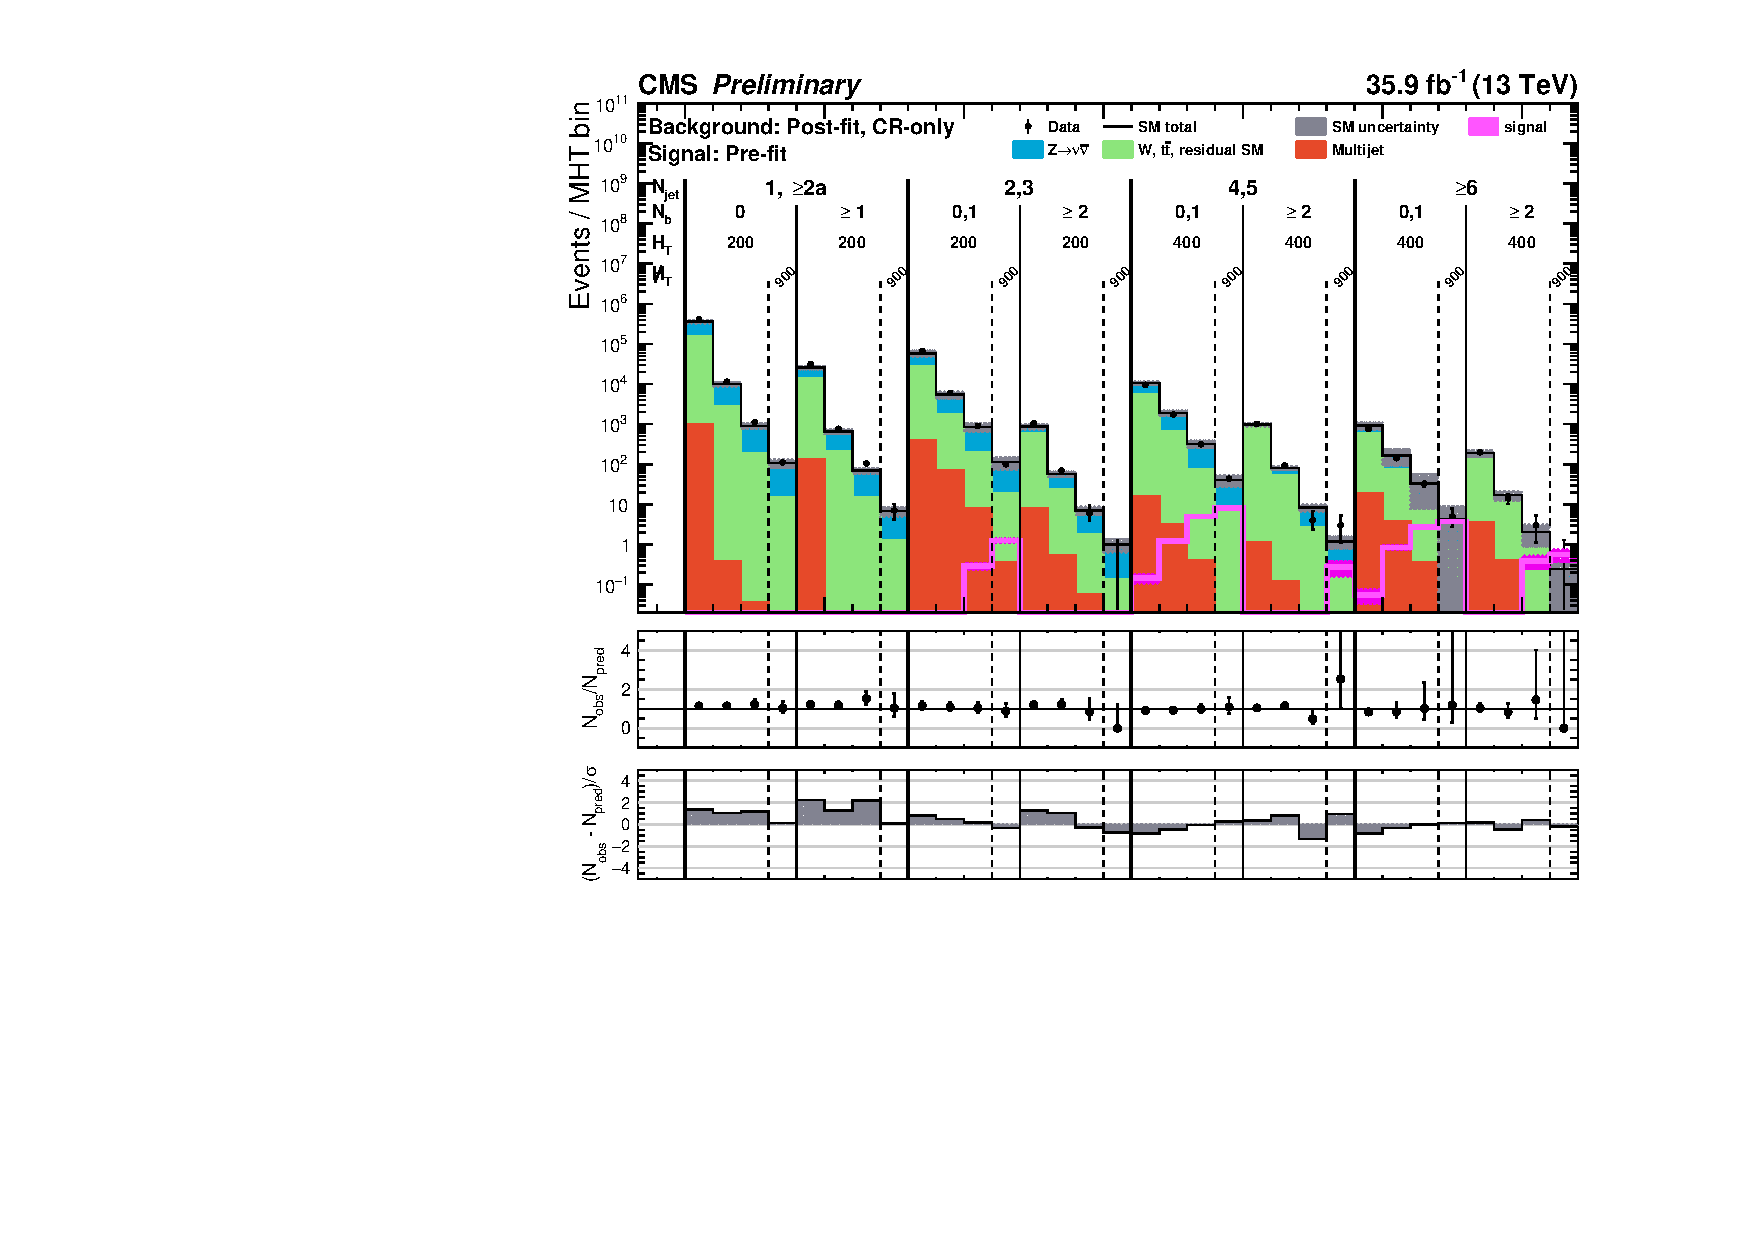
\includegraphics[width=0.49\textwidth]{figs/results/SMS-T1qqqqLL_ctau_0p001_mGluino-1800_mLSP-200_25ns_all_full-fit-sig}}~~
\subfloat[(0.001 mm, 1000 GeV, 
900 
GeV)]{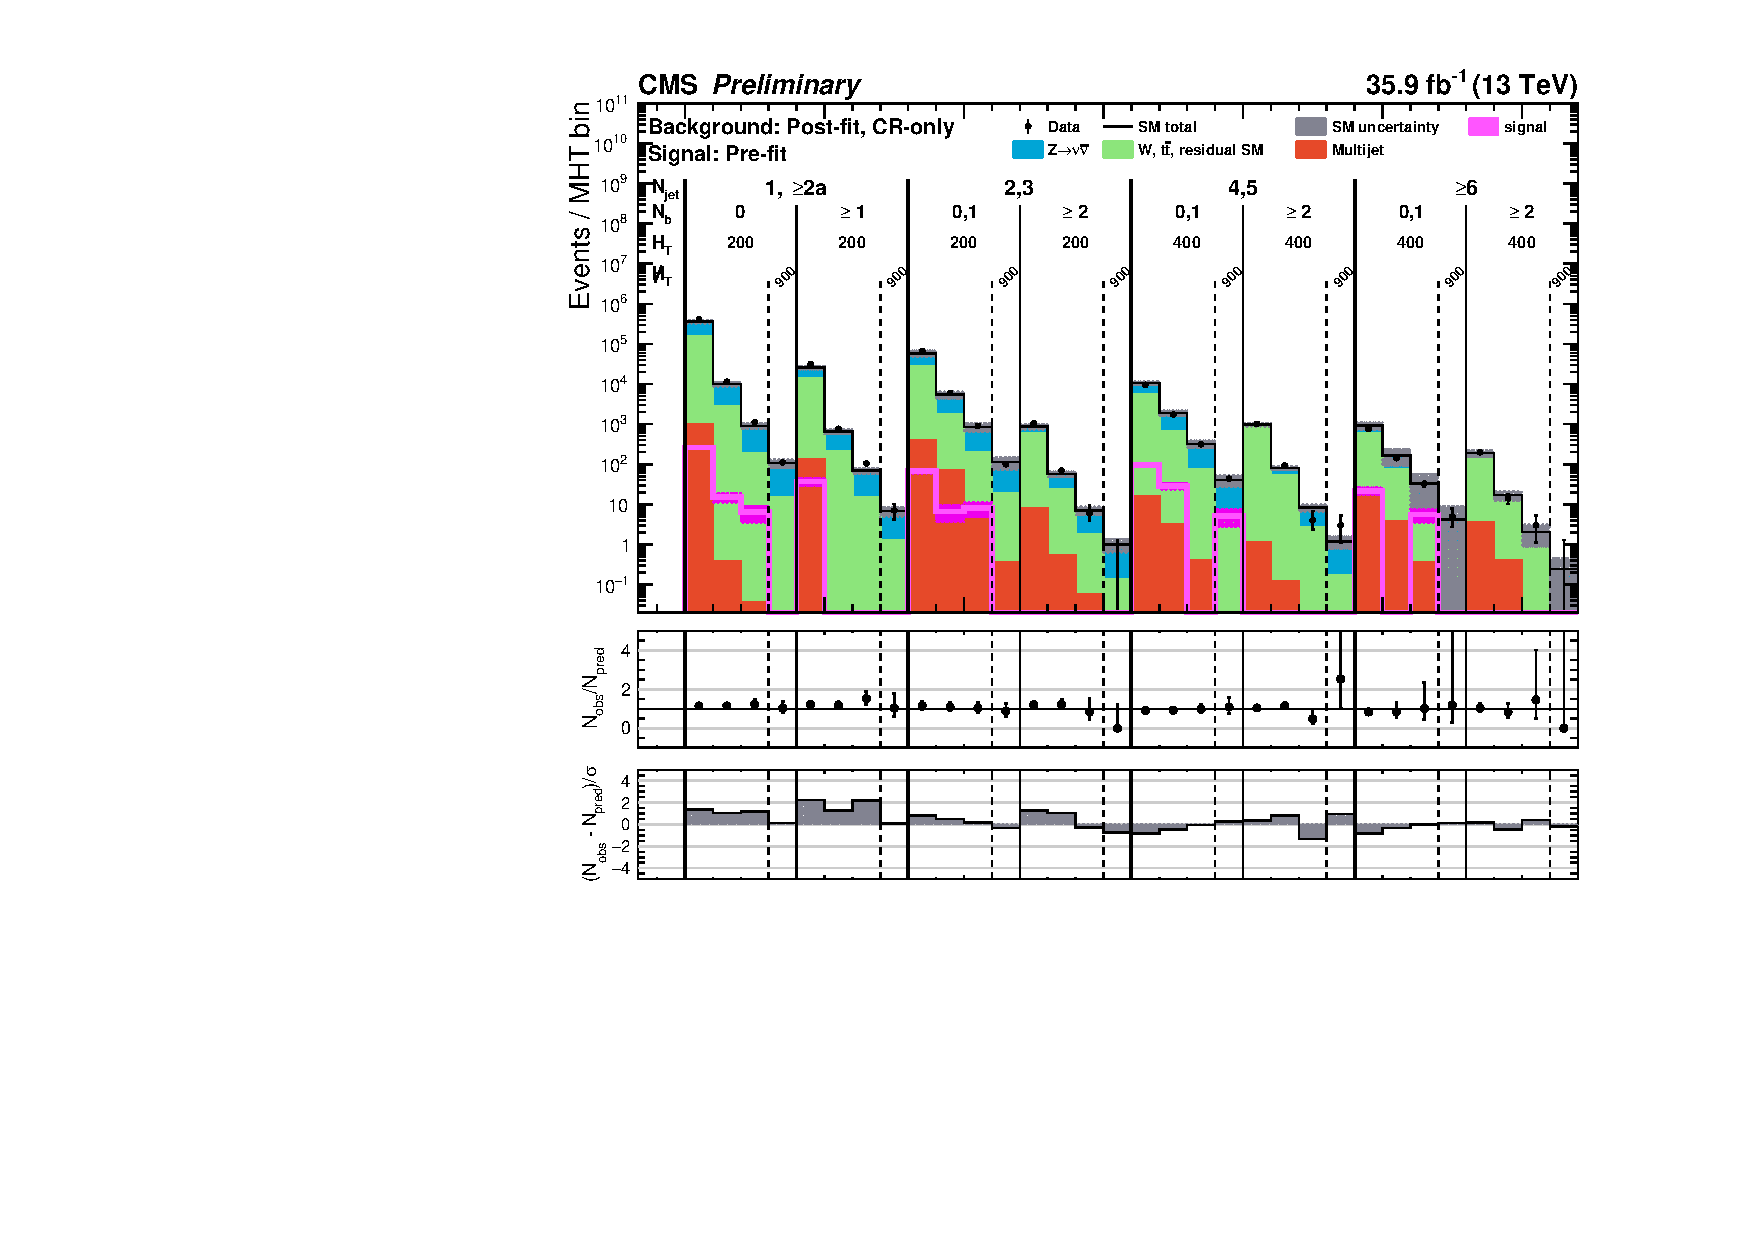
\includegraphics[width=0.49\textwidth]{figs/results/SMS-T1qqqqLL_ctau_0p001_mGluino-1000_mLSP-900_25ns_all_full-fit-sig}}\\
\subfloat[(1 mm, 1800 GeV, 
200 
GeV)]{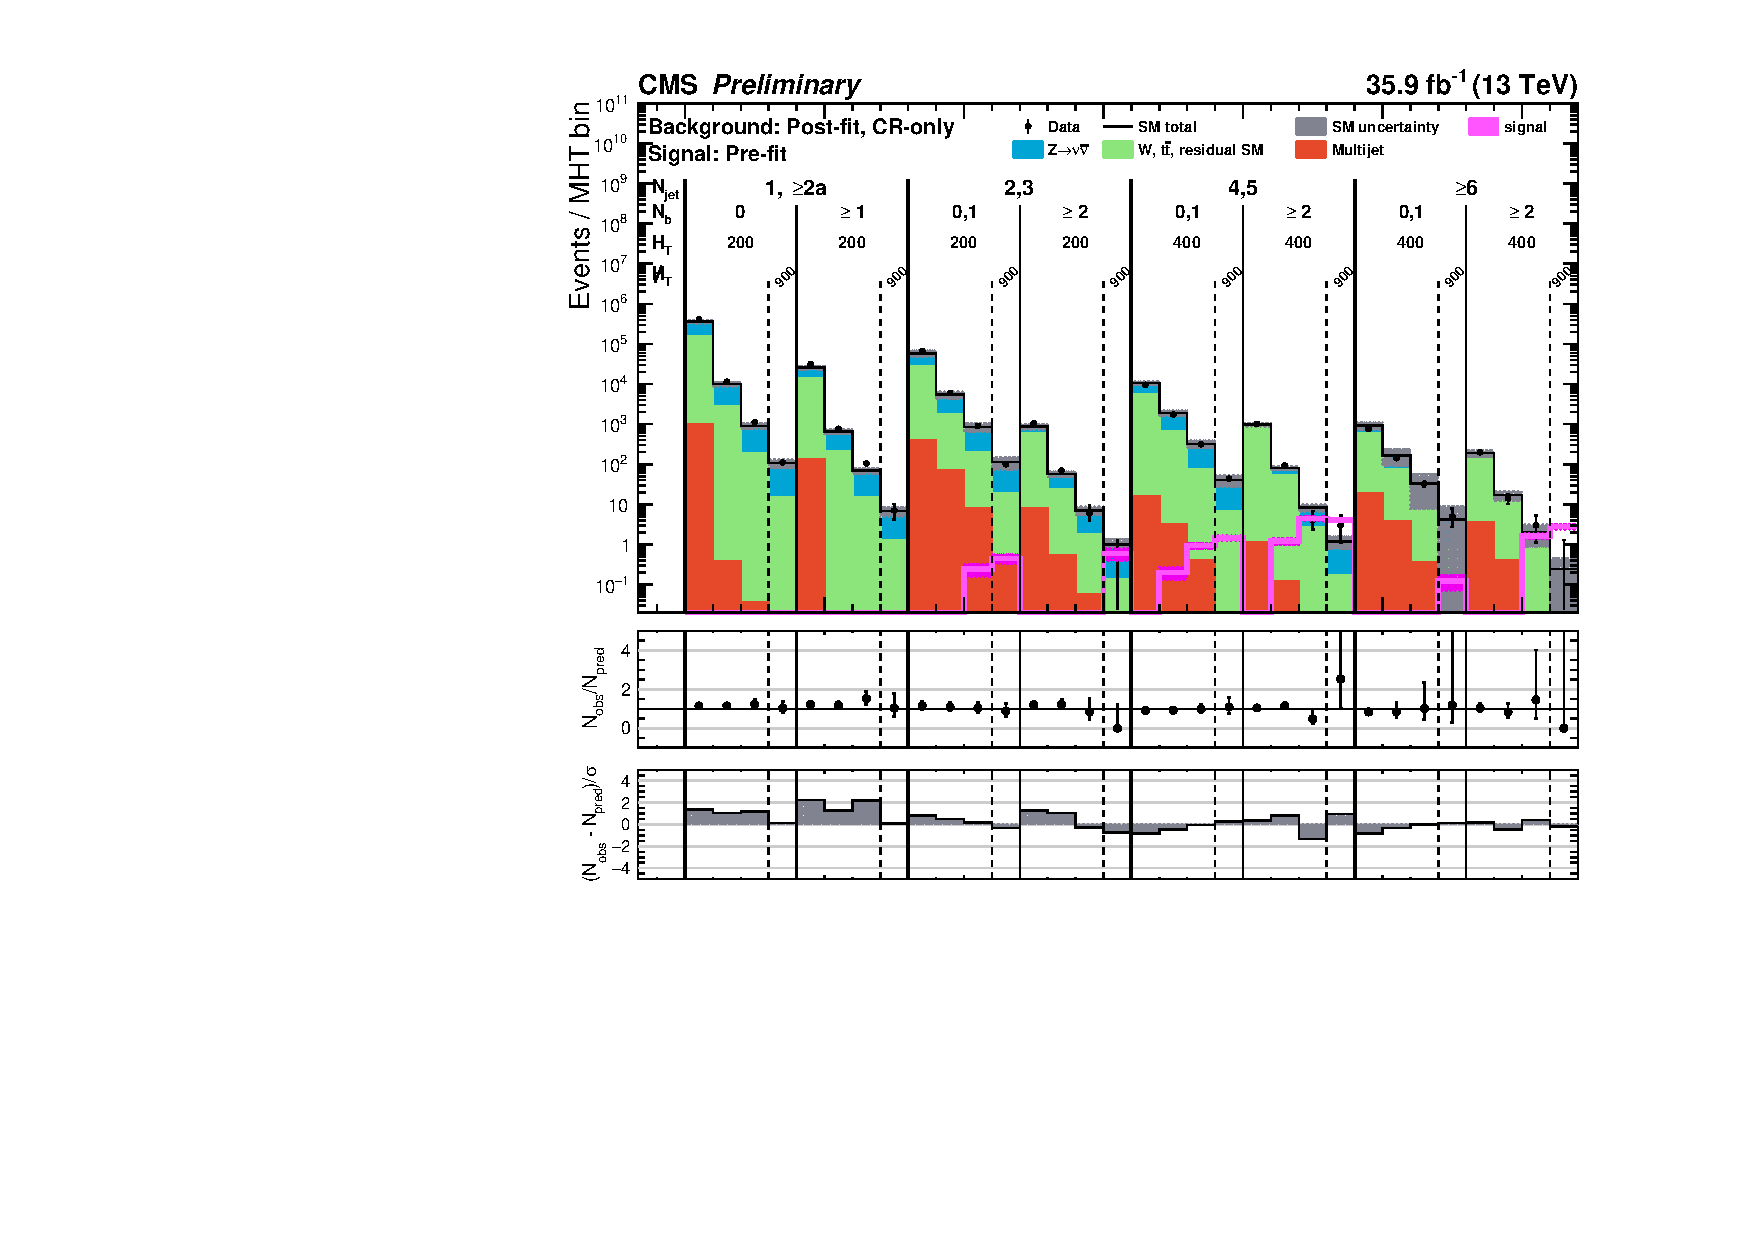
\includegraphics[width=0.49\textwidth]{figs/results/SMS-T1qqqqLL_ctau_1_mGluino-1800_mLSP-200_25ns_all_full-fit-sig}}~~
\subfloat[(1 mm, 1000 GeV, 
900 
GeV)]{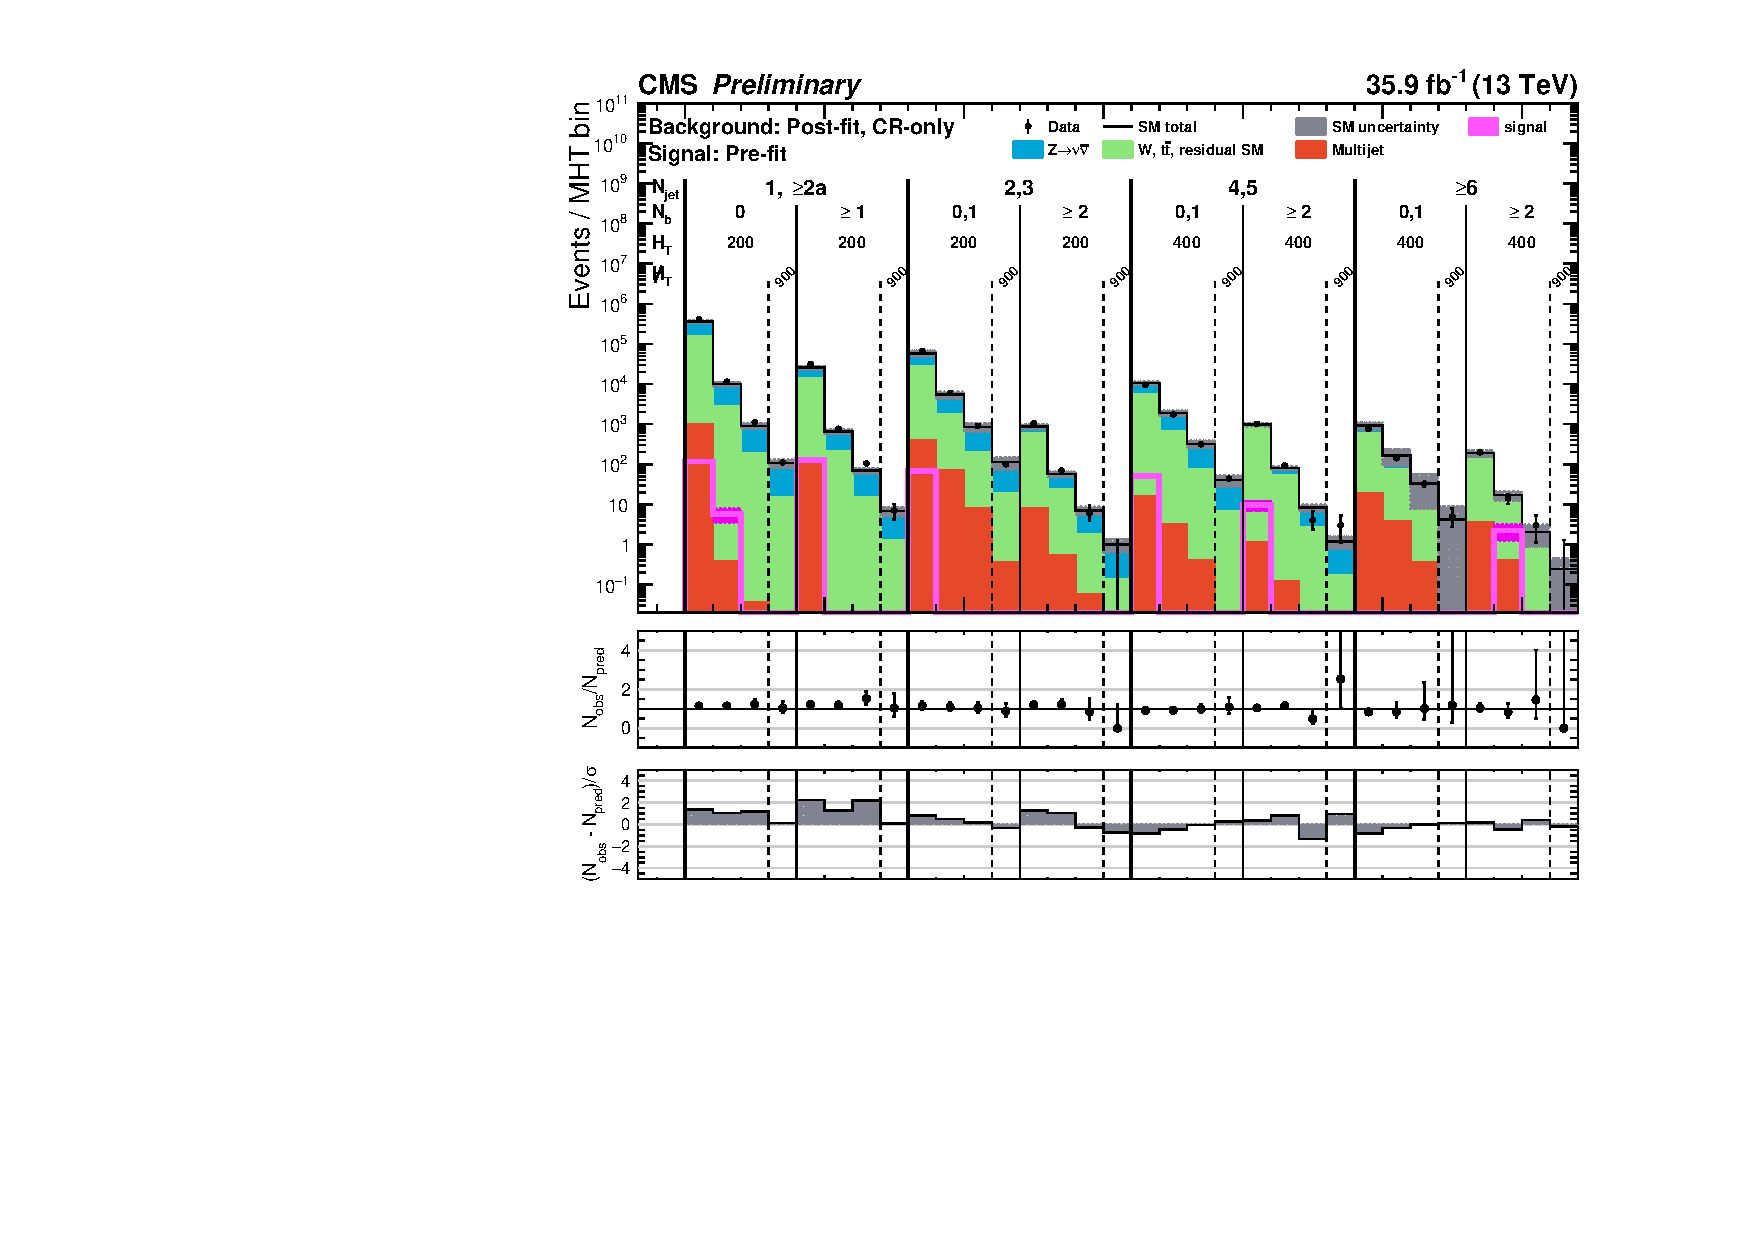
\includegraphics[width=0.49\textwidth]{figs/results/SMS-T1qqqqLL_ctau_1_mGluino-1000_mLSP-900_25ns_all_full-fit-sig}}\\
\subfloat[(100000 mm, 1000 GeV, 
200 
GeV)]{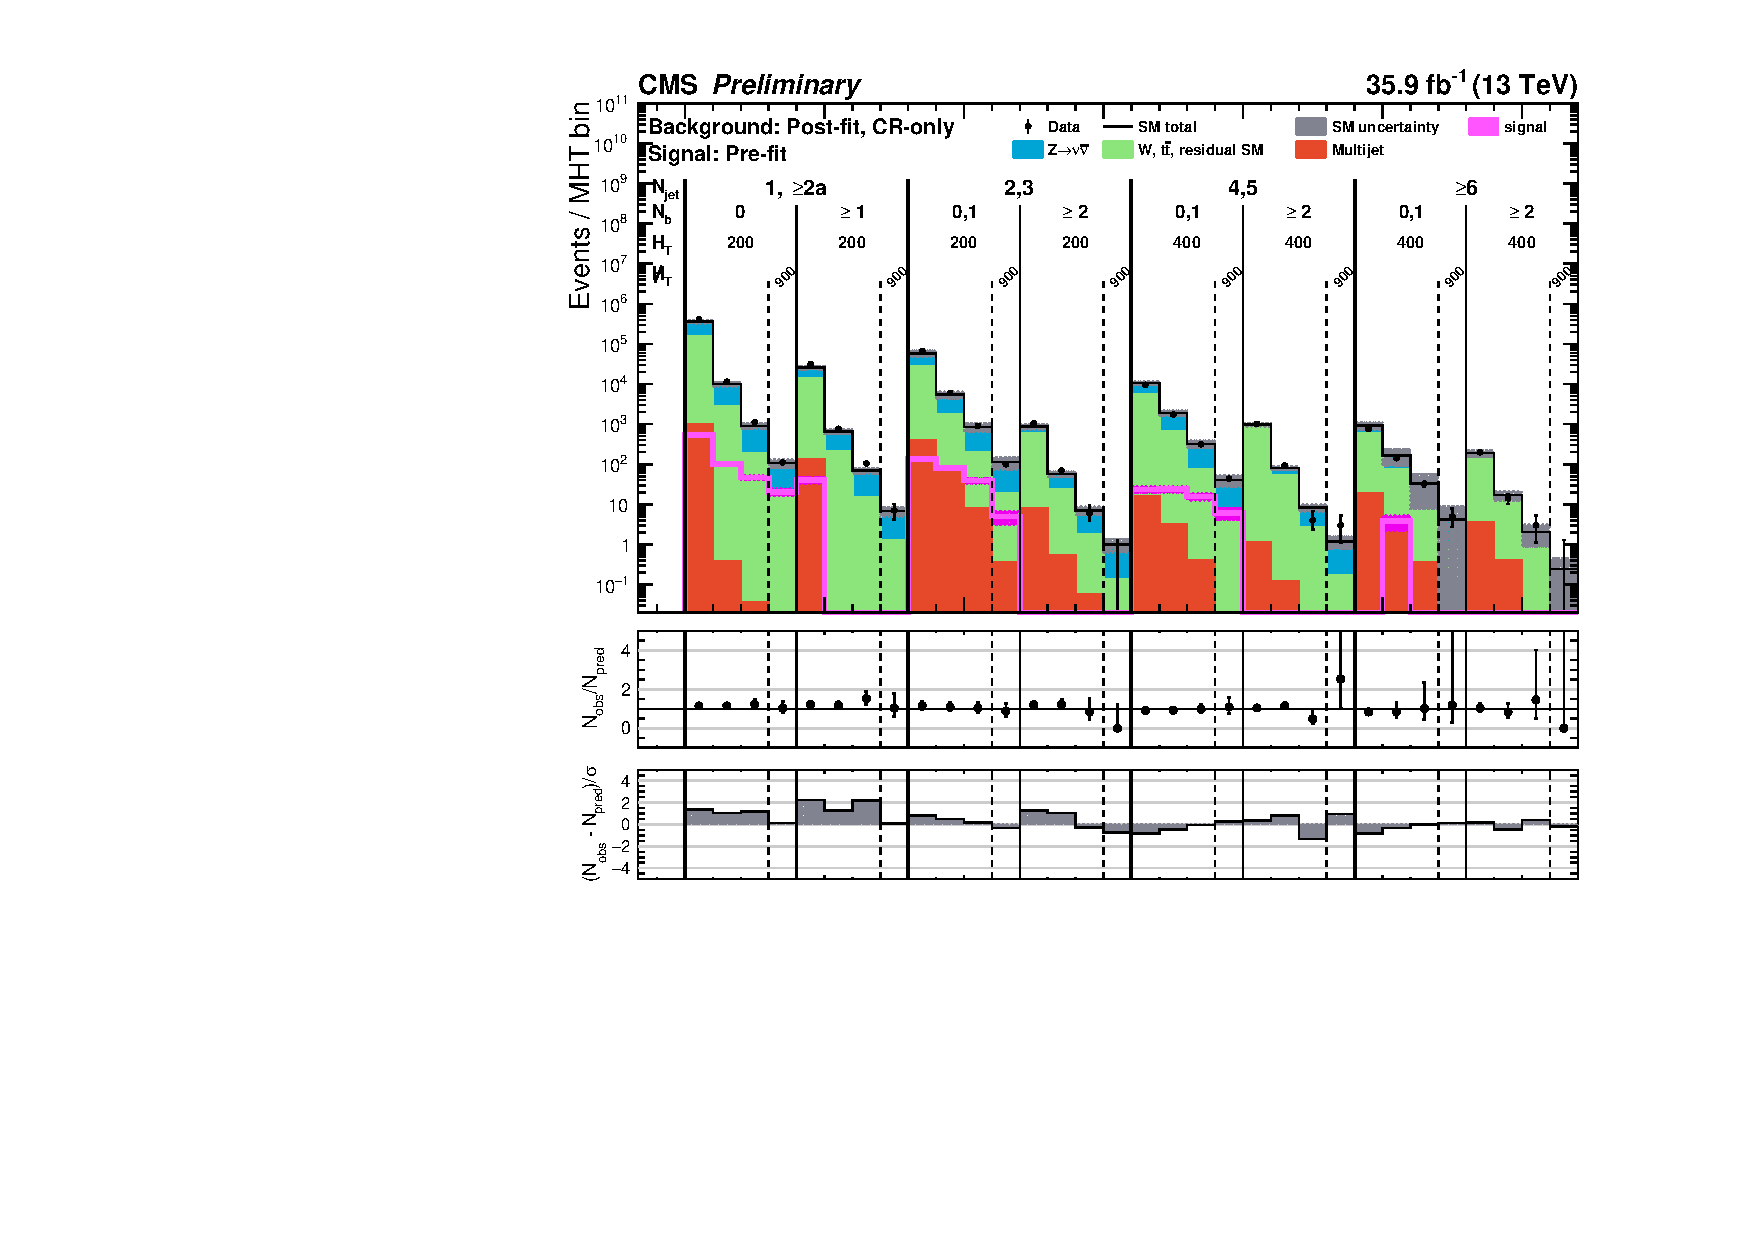
\includegraphics[width=0.49\textwidth]{figs/results/SMS-T1qqqqLL_ctau_100000_mGluino-1000_mLSP-200_25ns_all_full-fit-sig}}~~
\subfloat[(100000 mm, 1000 GeV, 
900 
GeV)]{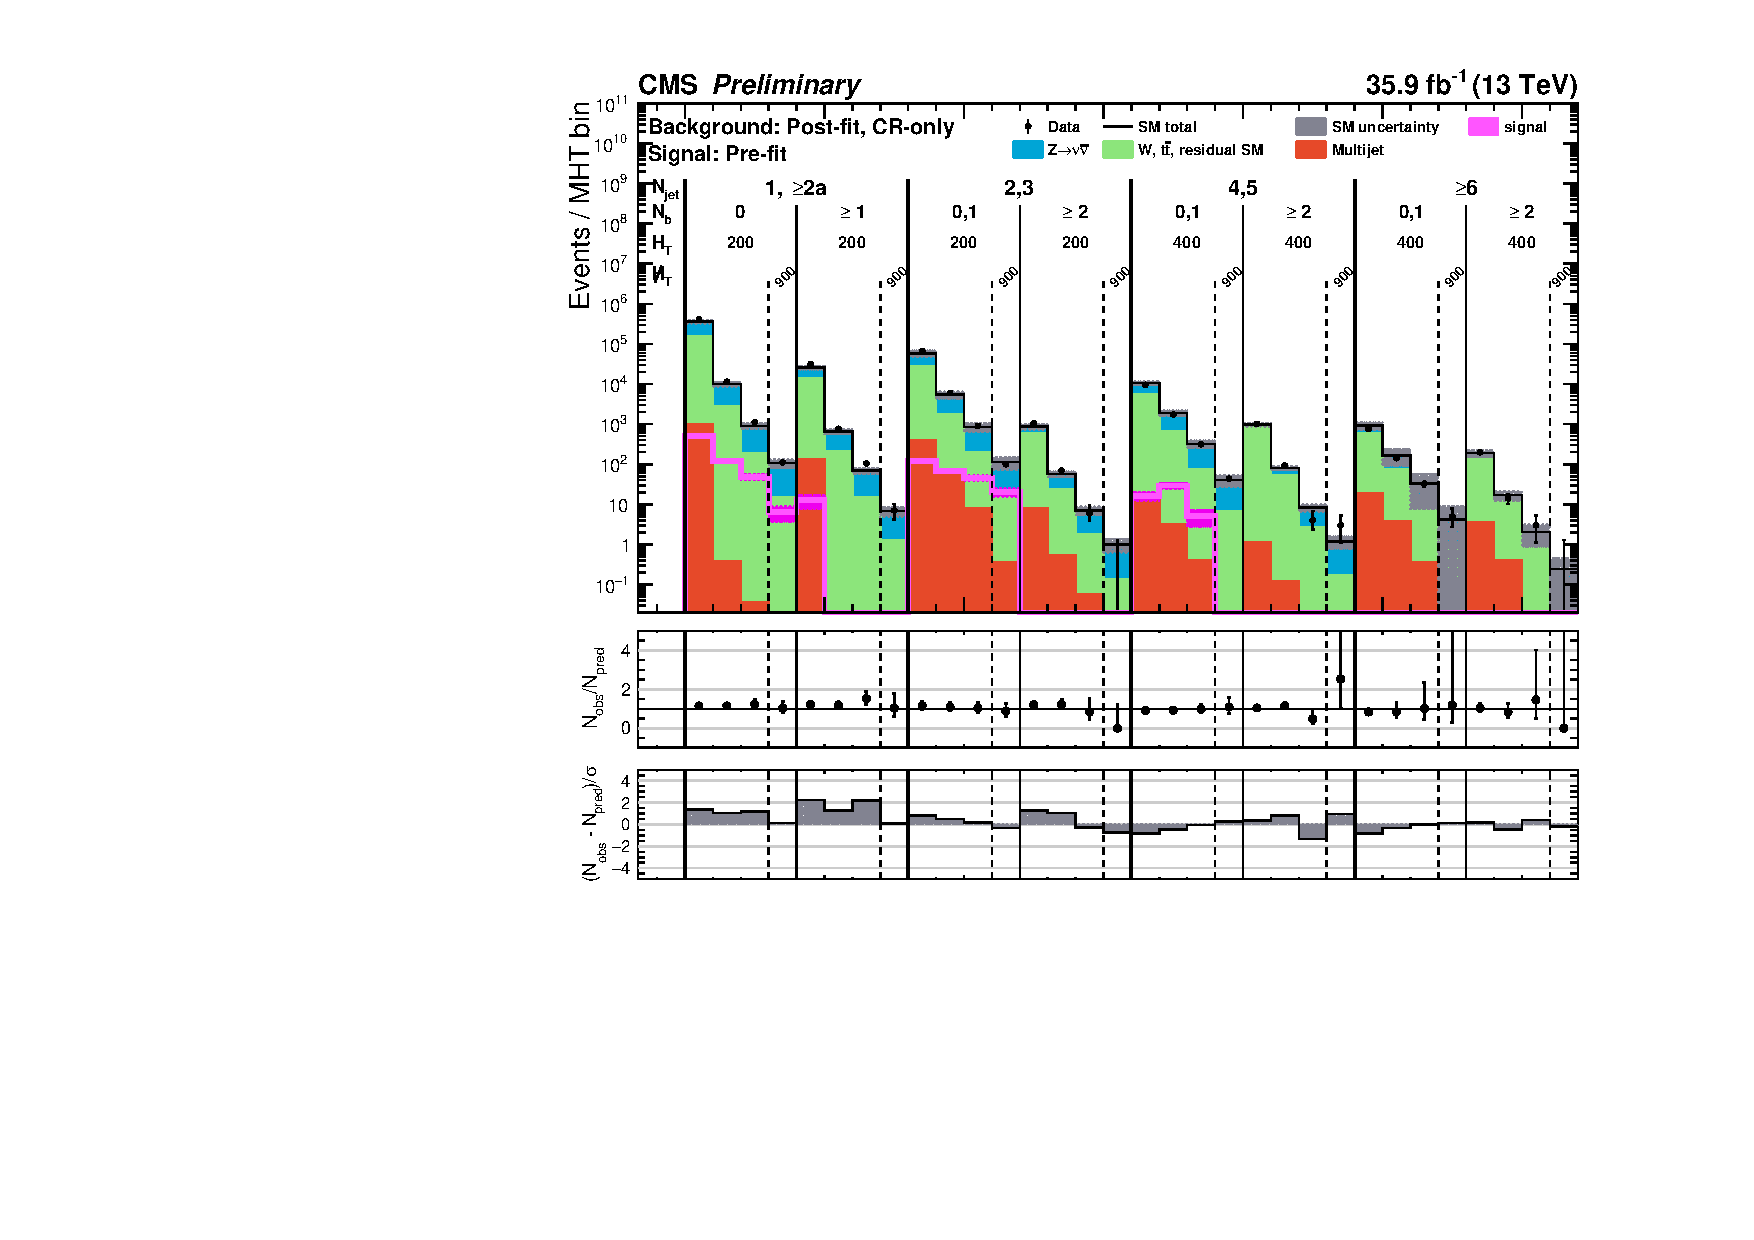
\includegraphics[width=0.49\textwidth]{figs/results/SMS-T1qqqqLL_ctau_100000_mGluino-1000_mLSP-900_25ns_all_full-fit-sig}}\\
\caption{Expected signal events for Split SUSY simplified models with a range 
of values of ($\ctau$, $\mglu$, $\mlsp$), overlaid on the expected standard 
model background counts, using an aggregated binning scheme.}
\label{fig:T1qqqqLL_MR}
\end{figure}


\section{Uncertainties on signal model simulation}
%1-2 pages.
%Similar to backgrounds.
%Luminosity, trigger, MC stat, pileup, b-tagging, JEC, ISR, genmet. 
The expected number of signal events is estimated using simulation. The various 
data-to-simulation correction factors discussed in 
Sec.~\ref{sec:analysis-mccorrections} are applied. The uncertainties in each 
\njnbhtmht bin are derived by varying the corrections within their 
uncertainties and recomputing the simulated yields, analogously to the 
uncertainties on the background processes 
(Sec.~\ref{sec:analysis-systematics-mht}). 
This includes uncertainties due to the corrections on the jet energy, pileup 
distribution, b-tagging efficiency, trigger efficiency, and ISR distribution. 
The integrated luminosity of 35.9~\ifb is measured with an uncertainty of 
2.5\%~\cite{lumi2016} which results in an additional uncertainty on the overall 
number of signal events. The statical uncertainties due the limited number of 
simulated events is also considered. Additional sources of uncertainty related 
to displaced jets are discussed in the remainder of this section. A summary of 
all sources of uncertainty and their typical sizes is shown in 
Tab.~\ref{tab:systs-signal} for various representative simplified models of 
long-lived gluino production.

%Summarise in table or words typical size of systs for relevant models.
\begin{table}[t]
\centering
\footnotesize
%\tiny
\begin{tabular}{c|cc|cc|cc}
\hline
& \multicolumn{2}{c|}{$\ctau=1~\micro\metre$} & \multicolumn{2}{c|}{$\ctau=1$ 
mm} & \multicolumn{2}{c}{$\ctau=10$ m} \\
Source of uncertainty & (1800,200) & (1000,900) & (1800,200) & 
(1000,900) & (1000,200) & (1000,900) \\   
\hline
Pileup & 1-3 & 1-3 & 2-4 & 1-4 & 1-5 & 1-5 \\
Jet energy scale & 3-9 & 4-14 & 3-9 & 4-17 & 4-9 & 2-12 \\
b-tagging & 0-1 & 0-1 & 17-59 & 10-41 & 0-1 & 0-1 \\
%b-tagging (heavy quark) &  &  & & & & \\
%b-tagging (light quark) &  &  & & & & \\
%b-tagging (long-lived) & & & & & & \\
Trigger & 3-4 & 0-2 & 2-4 & 0-2 & 0-4 & 0-1 \\
ISR & 3-5 & 2-10 & 2-5 & 2-9 & 2-14 & 3-14 \\
Luminosity & 2.6 & 2.6 & 2.6 & 2.6 & 2.6 & 2.6 \\
Stat. & 8-20 & 15-21 & 11-20 & 17-26 & 16-22 & 14-26 \\
\hline
\end{tabular}
\caption{Summary of uncertainties (\%) on the simplified long-lived gluino 
models for various values of ($\mglu$,$\mlsp$)~[GeV]. The 
quoted ranges correspond to the $\pm1\sigma$ quantiles of the yield changes 
across all \njnbhtmht bins.}
\label{tab:systs-signal}
\end{table}

%Additional systs for LL. make it subsection? no
%b-tagging, odd jet (chf, jet id), trigger.
%b-tagging: just one plot (integrated) but mention systs derived as a function 
%of pt and eta (same bins as btv).

%odd jet/chf
The requirement of \chf~$<0.1$ on the most energetic jet of the event, 
discussed in Sec.~\ref{sec:analysis-baselineselections}, reduces the selection 
efficiency for models with $1~\mathrm{m} \lesssim \ctau \lesssim 
10~\mathrm{m}$ to $\sim30\%$. This is because of the lack of reconstructed 
charged particle tracks in the displaced jets that are produced inside the 
calorimeters. 
For the same reason, the veto on events containing a jet that fails the 
identification requirements (which includes a minimum requirement on the 
charged component of jets), has a selection efficiency of $\sim10\%$ for these 
models.
Below and above this range in \ctau the efficiencies of the jet identification 
and \chf requirements are close to 100\%.
To account for a potential mismodelling of the simulation in the variables used 
for jet identification, the efficiency of these event selections are computed 
as a function of the decay lengths and pseudorapidities of the long-lived 
gluinos, and the sizes of the inefficiencies are propagated as a systematic 
uncertainty on the expected signal counts. 

%trigger
Jet identification requirements are also present in the trigger logic. The 
inefficiency of the trigger is measured to be at most 2\% for events with 
gluinos decaying within the calorimeter region. This is applied as a correction 
to the simulation, as a function of decay length and pseudorapidity, and an 
appropriate systematic uncertainty is assigned.
% syst is the same as the nominal systs measured (2-3%) (derived from muons vs 
%%electron reference triggers as a function of mht)

%b-tagging
As seen in the previous section, jets with a displacement of $\sim1$~mm can be 
tagged by the b-tagging algorithm. This is because they have similar 
displacements as b-quarks.
The b-tagging efficiency for displaced jets is measured as a 
function of the displacement $d$ with respect to the primary vertex, in bins of 
$\pt$ and $\eta$, and compared to the 
efficiency for standard model quarks. An example of this is shown in 
Fig.~\ref{fig:LL-btagging}. 
% displacement is 3D, particle's reference frame to acount for the different 
%Lorentz boosts of the gluinos and b quarks.
% ttbar sample used, no cuts, no BTV scale factors applied
Three regions are identified as $d<0.1$~mm (small displacements), $d>10$~mm 
(large displacements), and $0.1<d<10$~mm (``b-like'' displacements). In the 
$0.1<d<10$~mm region, the b-tagging efficiency for displaced jets is 
approximately 60\%, almost comparable to that for b-quarks ($\sim80$\%). The 
nominal b-tagging correction factors and uncertainties (described in 
Sec.~\ref{sec:analysis-mccorrections-btagging}) are applied in the simulation 
to jets with this range of displacements, together with an additional 
uncertainty of size 20-50\% to cover differences in the efficiencies with 
respect to jets originating from b-quarks. For displacements of $d<0.1$~mm and 
$d>10$~mm, the efficiency falls to 1-5\%, similar to that of light quarks. A 
conservative 100\% uncertainty on the efficiency is taken in these regions.
%% b-tagging syst is of course split into 4 (heavy, light, LL b-like, LL 
%%light-like)

\begin{figure}[h]
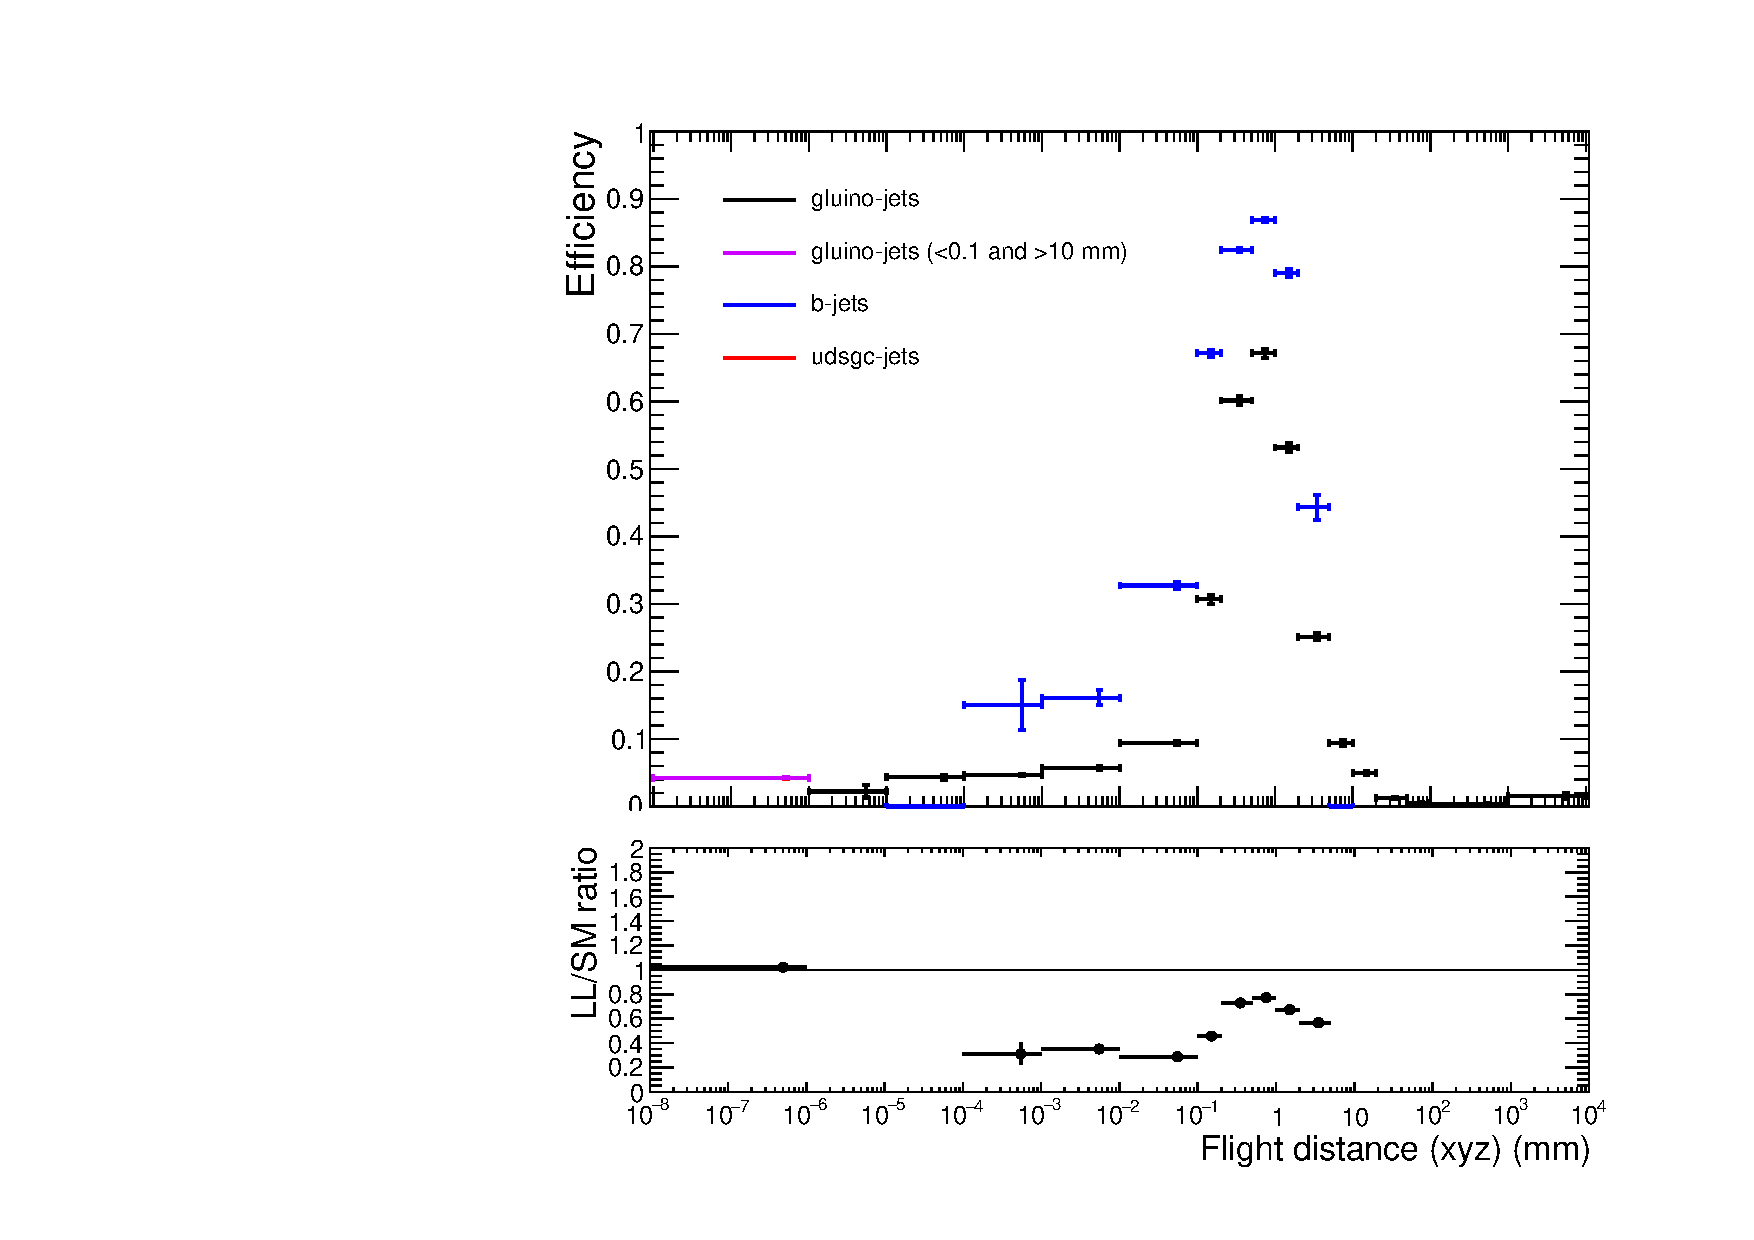
\includegraphics[width=0.75\textwidth]{figs/results/btageff_proper_compressed_pt100_eta0}
\caption{Efficiency of the b-tagging algorithm for displaced jets originating 
from long-lived gluinos, compared to standard model bottom and light quarks, 
for jets with $100 < \pt < 140$ and $0 < |\eta| < 0.5$.}
%As light quarks have a negligible decay length, these The first bin in the 
%histogram, which is inclusive with respect to displacement.}
\label{fig:LL-btagging}
\end{figure}


\section{Statistical model}
\label{sec:results-likelihoodmodel}
%2-3 pages.
%Used to incorporate background estimations and uncertainties and compare 
%whether B-only or B+S fits data better.
In order to perform a statistical analysis of the results obtained, a 
likelihood function is used to model the background and signal events across 
the \njnbhtmht parameter space in the signal and control regions, accounting 
for all relevant uncertainties. The 
likelihood function is utilised to carry out the background estimation as well 
as to perform hypothesis tests to assess the sensitivity of the search to new 
physics.
%Model the bins and number of events and uncertainties and correlations between 
%bins as a likelihood function (probability of observing the observed data 
%given 
%some model parameters). This will then be fitted/maximised/used to make the 
%background estimations and perform statistical tests to determine limits.

The number of events in each bin of the \njnbhtmht parameter space is modelled 
as a Poisson distribution, with an expected value given by that obtained from 
simulation, multiplied by \textit{modifier} terms that account for the transfer 
factors and relevant uncertainties. The uncertainties are encoded as 
\textit{nuisance parameters} with probability densities and correlations that 
will be discussed in this section.

The component of the likelihood function related to the \njnbht bin $k$ in the 
signal region is given by:
\begin{equation}
\mathcal{L}_\mathrm{sig}^k = \prod_{j} \mathcal{P}\left( n_\mathrm{sig}^{k,j} 
\bigg\rvert \sum_{i} (
b_\mathrm{Z,sig}^{i,j} r_{\mathrm{Z}}^i \theta_\mathrm{Z,sig}^{i,j} + 
b_\mathrm{W,sig}^{i,j} r_{\mathrm{W}}^i \theta_\mathrm{W,sig}^{i,j} + 
b_\mathrm{QCD,sig}^{i,j} \theta_\mathrm{QCD,sig}^{i,j} +
\mu_s s_\mathrm{sig}^{i,j} \theta_{s,\mathrm{sig}}^{i,j}
) \right) \, ,
\end{equation}
where the product is over all \mht bins within the \njnbht bin, 
$n_\mathrm{sig}^{k,j}$ is the number of events observed in data in a given 
\njnbhtmht  
bin, the summation is over all fine \njnbht bins $i$ that form part of the 
given coarse \scalht bin (Sec.~\ref{sec:analysis-binning}), 
$b_\mathrm{Z,sig}^{i,j}$ 
and $b_\mathrm{W,sig}^{i,j}$ are the number of \znnj and \ttw events expected 
based on simulation, $r_{\mathrm{Z}}^i$ and $r_{\mathrm{W}}^i$ are the control 
region based
data-to-simulation correction ratios in the transfer factor equations 
(Eq.~\ref{eqn:estimation2}), $\theta_\mathrm{Z,sig}^{i,j}$ and 
$\theta_\mathrm{W,sig}^{i,j}$ encapsulate all relevant 
uncertainties related to the transfer factors (both from the data-driven 
closure tests and the variations in simulation), the \mht shape, and the 
limited number of 
simulated events, $b_{\mathrm{QCD},\mu}^i$ is the number of QCD events 
estimated using the method described in Sec.~\ref{sec:analysis-estimation-qcd} 
with $\theta_\mathrm{QCD,sig}^{i,j}$ encoding its uncertainty, 
$s_\mathrm{sig}^{i,j}$ is the expected number of signal 
events based on simulation with $\theta_{s,\mu}^i$ encapsulating its 
uncertainties, 
and $\mu_s=\frac{\sigma}{\sigma_{\mathrm{th}}}$ is a signal strength parameter 
that scales the signal model's cross section with respect to its theoretical 
value and is relevant when setting limits (Sec.~\ref{sec:results-limitsproc}).

The component of the likelihood function related to the \njnbht bin $i$ in the 
\mj control region is given by:
\begin{equation}
\mathcal{L}_\mu^i = \mathcal{P}\left( n_\mu^i \bigg\rvert 
b_\mu^i r_{\mathrm{W}}^i \theta_{b,\mu}^i + 
b_{\mathrm{QCD},\mu}^i + 
\mu_s s_\mu^i \theta_{s,\mu}^i \right) \, ,
\end{equation}
in which the small potential contributions from QCD and signal events are 
accounted for (based on the simulation). 
%where $n_\mu^i$ is the number of events observed in data in that bin, 
%$b_\mu^i$ is the number of events expected based on simulation, 
%$r_{\mathrm{W}}^i$ is the data-to-simulation correction ratio in the transfer 
%factor equation (Eq.~\ref{eqn:estimation2}), $\rho_{b,\mu}^i$ encapsulates all 
%relevant uncertainties related to the transfer factors (both from the 
%data-driven closure tests and the variations in simulation) and the limited 
%number of simulated events, $b_{\mathrm{QCD},\mu}^i$ is the small number of 
%QCD 
%events which is taken from simulation, $s_\mu^i$ is the expected number of 
%signal events based on simulation and $\rho_{s,\mu}^i$ encapsulates its 
%uncertainties, and $\mu$ is a signal strength parameter that scales the signal 
%model's cross section and is relevant when setting limits).
%signal contam.
Similarly, the likelihood in the \mmj control region is written as:
\begin{equation}
\mathcal{L}_{\mu\mu}^i = \mathcal{P}\left( n_{\mu\mu}^i \bigg\rvert 
b_{\mu\mu}^i r_{\mathrm{Z}}^i \theta_{b,\mu\mu}^i + 
b_{\mathrm{QCD},\mu\mu}^i + 
\mu_s s_{\mu\mu}^i \theta_{s,\mu\mu}^i \right) \, .
\end{equation}

The correction parameters $r_{\mathrm{Z}}^i$ and $r_{\mathrm{W}}^i$ are shared 
between the signal region and relevant control region. These parameters are 
unconstrained (they are modelled by a uniform distribution) and therefore allow 
the background estimations to be made when maximising the likelihood function 
over the control regions.
%In the \mmj control region, the $r_{\mathrm{Z}}^i$ parameters are the same in 
% ACTUALLY not true this is what lucien did at one point but it's wrong (you're 
%not binning in nb=0,ge1 then, but then changed it to really integrate over 
%nb>=1)

Each source of uncertainty (described in Sec.~\ref{sec:analysis-systematics}) 
results in an uncertainty on the expected number of events of 
a given process in each bin of the search. 
The correlations of the uncertainties between bins are included in the 
likelihood function and, for simplicity, are chosen to be either 
0 (uncorrelated) or 1 (perfectly correlated). As a simple 
example, a correlation of 1 between two bins, each with a (different) expected 
number of event counts and associated uncertainty, means that if the counts in 
one bin are increased by one standard deviation, the counts in the other bin 
also increase by one standard deviation. This is implemented in the likelihood 
model such that bins that are assumed to be fully correlated share the same 
nuisance parameter, whereas bins that are uncorrelated have independent 
nuisance parameters.

The nuisance parameters representing the systematic uncertainties derived from 
the data-driven closure tests (Sec.~\ref{sec:analysis-systematics-data}) %, as 
%well as those on the estimated QCD background, 
are modelled as a log-normal distribution. As these are derived in turn as a 
function of \njet and \scalht, integrated over the other dimensions, and are 
statistical in nature, two sets of nuisance parameters are included that are 
considered to be correlated across the \nb, 
\scalht and \mht (\njet, \nb and \mht) dimensions and uncorrelated in \njet 
(\scalht). 
%Adam: Since the uncertainties derived with this approach are statistical in 
%nature, these systematics are considered uncorrelated in each HT bin and event 
%topology category.
%Matt: Theyare considered as uncorrelated per HT and jet topology (monojet and 
%asymmetric topologies are correlated) and correlated in other categorisations.

The systematic uncertainties derived on the \mht shape 
(Sec.~\ref{sec:analysis-systematics-mht}) are incorporated as $\pm1\sigma$ 
alternative \mht distributions. The event yields in each bin of the 
distributions are interpolated quadratically between the alternative shapes and 
extrapolated linearly beyond this. This ``morphing'' procedure is controlled by 
a Gaussian nuisance parameter, and is described in Ref.~\cite{templatemorphing}.
%vertical template morphing
%correlation in njet and ht (see AN p50).
Two sets of uncertainties are derived on the \mht distributions, by performing 
the linear fits described in Sec.~\ref{sec:analysis-systematics-mht} 
integrating over \scalht and \njet in turn. This results in two sets of  
uncertainties that are correlated in \scalht and \njet, respectively, and are 
derived for each of the \znnj (from the \mmj control region fit) and \wlj (from 
the \mj control region fit) processes.

Similarly, the systematic uncertainties derived from variations of the 
data-to-simulation correction factors (Sec.~\ref{sec:analysis-systematics-mc}) 
are also incorporated as alternative \mht distributions in the signal region. 
In this case, these may also change the \mht normalisation and therefore affect 
the transfer factors. In the control regions there is effectively no \mht shape 
as they are not binned in this variable.
Each of these uncertainties is assumed to originate from a unique 
underlying source, and so they are treated as being fully correlated across the 
full parameter space of the signal and control regions. In other words, there 
is only one nuisance parameter for each source of uncertainty that is shared 
among all bins and processes.
%and so the effect of each source is varied assuming a fully correlated 
%behaviour across the full 1163 phase space of the signal and control regions.

%%% bbb light (otherwise too many parameters)
The statistical uncertainties due to the limited number of simulated events are 
modelled as a Gaussian distribution in each bin, and are uncorrelated across 
bins. Finally, the QCD estimate in the signal region is assigned a conservative 
100\% uncertainty, modelled as a log-normal distribution, that is uncorrelated 
across \njet and \scalht and correlated across \nb and \mht.

The probability densities of the nuisance parameters %and their correlations
are encoded within the likelihood function $\mathcal{L}_\mathrm{nuis}$.
The total likelihood for all bins in the signal and control regions and their 
uncertainties is then given by the product:
\begin{equation}
\mathcal{L} = \mathcal{L}_\mathrm{nuis} \prod_k \mathcal{L}_\mathrm{sig}^k 
\prod_i \mathcal{L}_{\mu}^i \prod_i \mathcal{L}_{\mu\mu}^i
\end{equation}

%Maybe describe how minimisation is done (gradient descent bla migrad bla).

%Refer back to big syst table (maybe modify it and add correlations)
%Correlation scheme (go back and fix up in systs section)
%i would just mention correlation scheme in this section (have a paragraph).


%\section{Results under the background-only hypothesis}
\section{Comparison of expected background and observed data}
\label{sec:results-results}
%3-5 pages.
%CR fit ("predictions") (basically applying TF equations) and full fit 
%(background-only).
%CR-only for predictions (expected background) and inspect comparison with SR, 
%full fit to compare likelihood under B-only and B+S (for limits)
As will be discussed in Sec.~\ref{sec:results-limitsproc}, the sensitivity of 
the search is assessed by 
comparing the values of the maximised likelihood function under the 
background-only hypothesis ($\mu_s=0$) and the background-plus-signal 
hypothesis ($\mu_s \ne 0$). First, it is instructive to compare the observed 
event counts in 
data with those expected from the standard model. The expected standard model 
background is obtained by performing the maximum likelihood fit under the 
background-only hypothesis to the control regions only (i.~e.~the signal region 
is excluded). This is essentially equivalent to the application of the transfer 
factor equations (Sec.~\ref{sec:analysis-estimation-ewk}).
% except for nb extrapolation (otherwsie yes, saturated model and rate params 
%equal data/mc

The results of this fit are shown in 
Figs.~\ref{fig:results1}~and~\ref{fig:results2}.
These show the observed number of events in data and the expected number of 
Z, \ttw and QCD background events in every \njnbhtmht bin of the signal 
region. The uncertainties on the background expectation include both the 
systematic and statistical components added in quadrature. 
Also shown are the ratios in each bin between the observed and expected number 
of events, and the z-scores (the difference between observed and expected 
counts, divided by the uncertainty on the expected counts).
The ratios and z-scores, integrated over \mht, are also summarised in 
Fig.~\ref{fig:ratios_and_pulls}.
The observed and expected event counts are also summarised in tabulated form in 
App.~\ref{app:results-results}.

Overall, no statistically significant excess is observed in the data.
The z-scores are found to be centred on zero, with almost all bins having 
values within $\pm2\sigma$.
Similarly, the ratios of observed and expected counts are consistent with unity.
%No statisticallyl significant (all less than 2 sigma) excess observed hence 
%set limits. ratios close to 1, pulls centred on 0

A likelihood fit is also performed under the background-only hypothesis to the 
full control and signal region parameter space. The results of this are shown 
in App~\ref{app:results-fullfit}.
Again, the binned observed number of events is found to be consistent, within 
uncertainties, with those expected from the standard model. The best fit values 
of the nuisance parameters are shown in App.~\ref{app:nuisances} and can be 
seen to be within their $\pm1\sigma$ values.

%Mountain range plots (2 pages).
%Distributions of pulls.
%Pulls on nuisances? app
%Tabulated counts? app

\begin{figure}[!p]
\centering
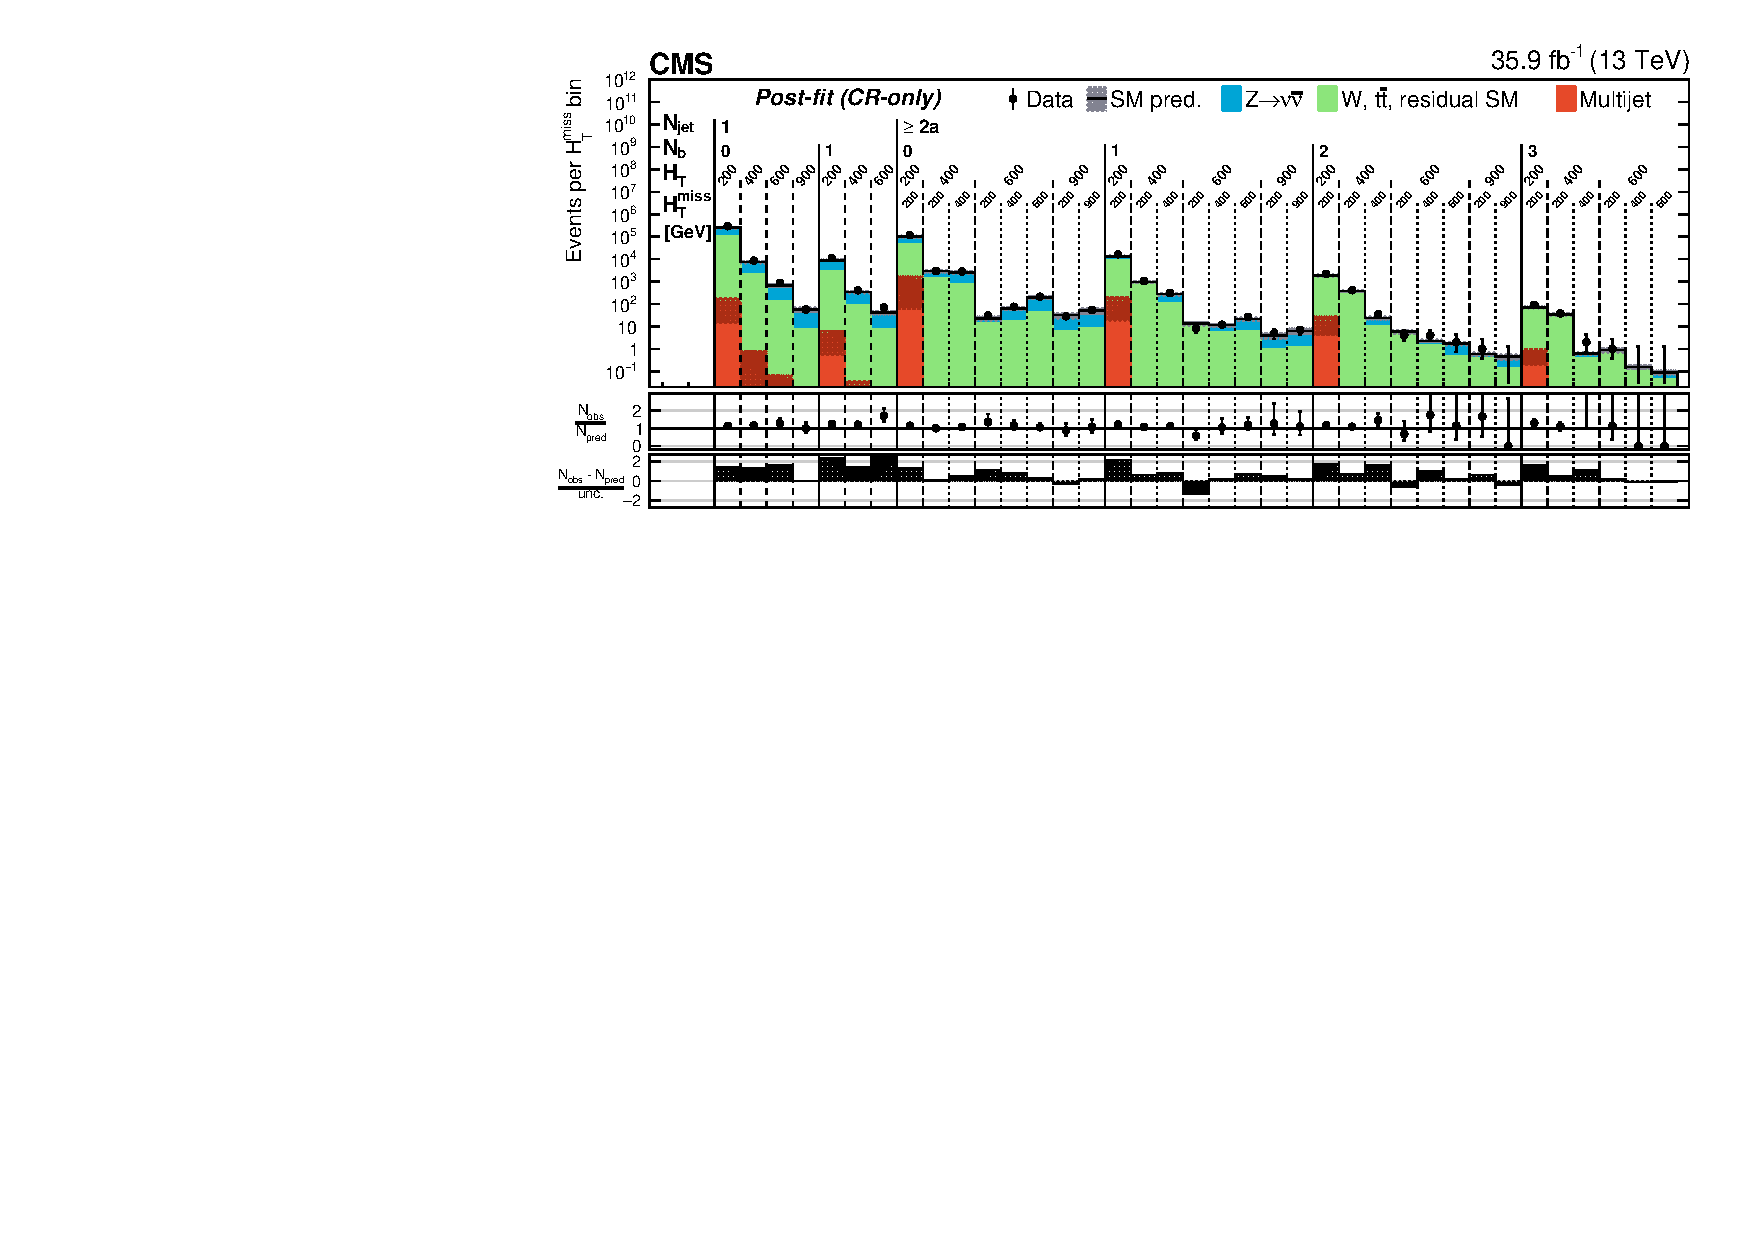
\includegraphics[width=0.99\textwidth, trim=0 0 0 0, 
clip=true]{figs/results/1jet_cr-only.pdf}\\
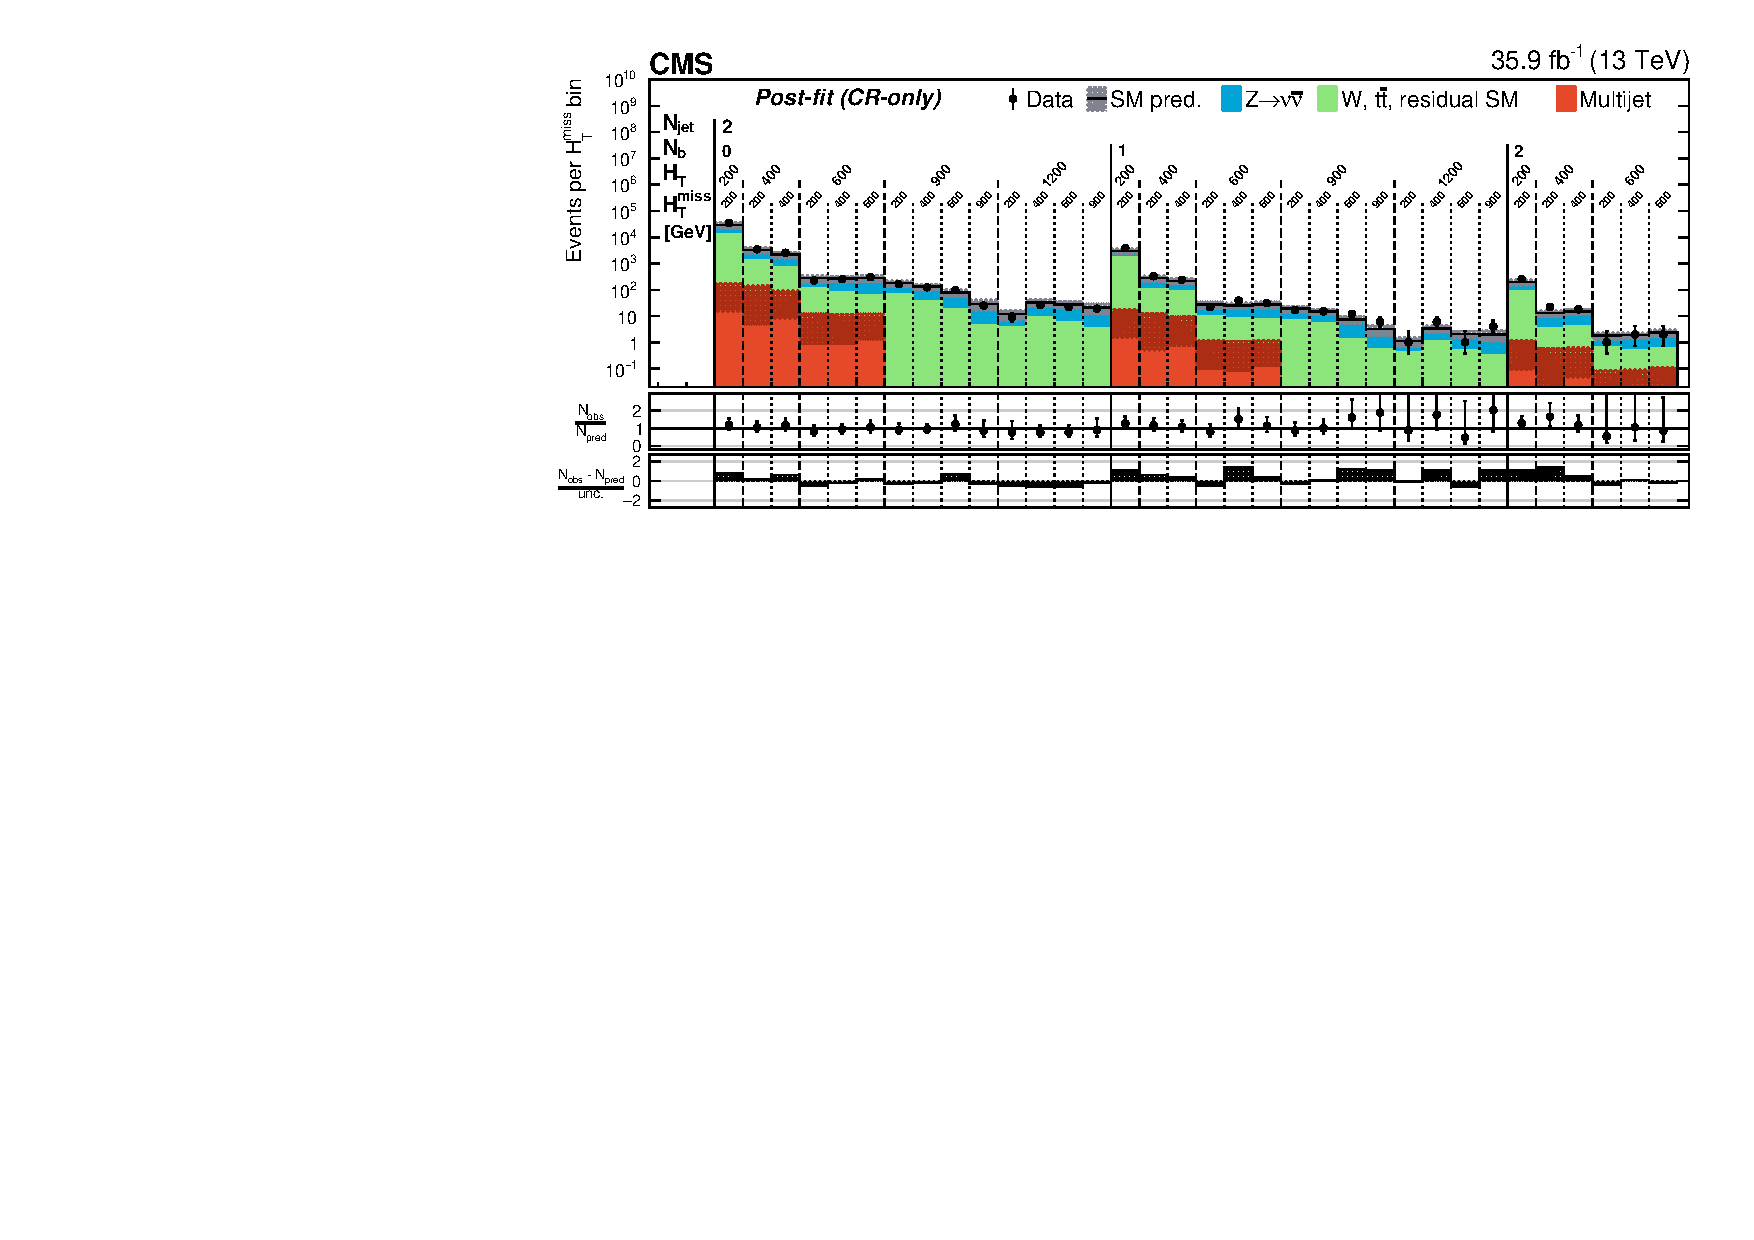
\includegraphics[width=0.99\textwidth, trim=0 0 0 0, 
clip=true]{figs/results/2jet_cr-only.pdf}\\
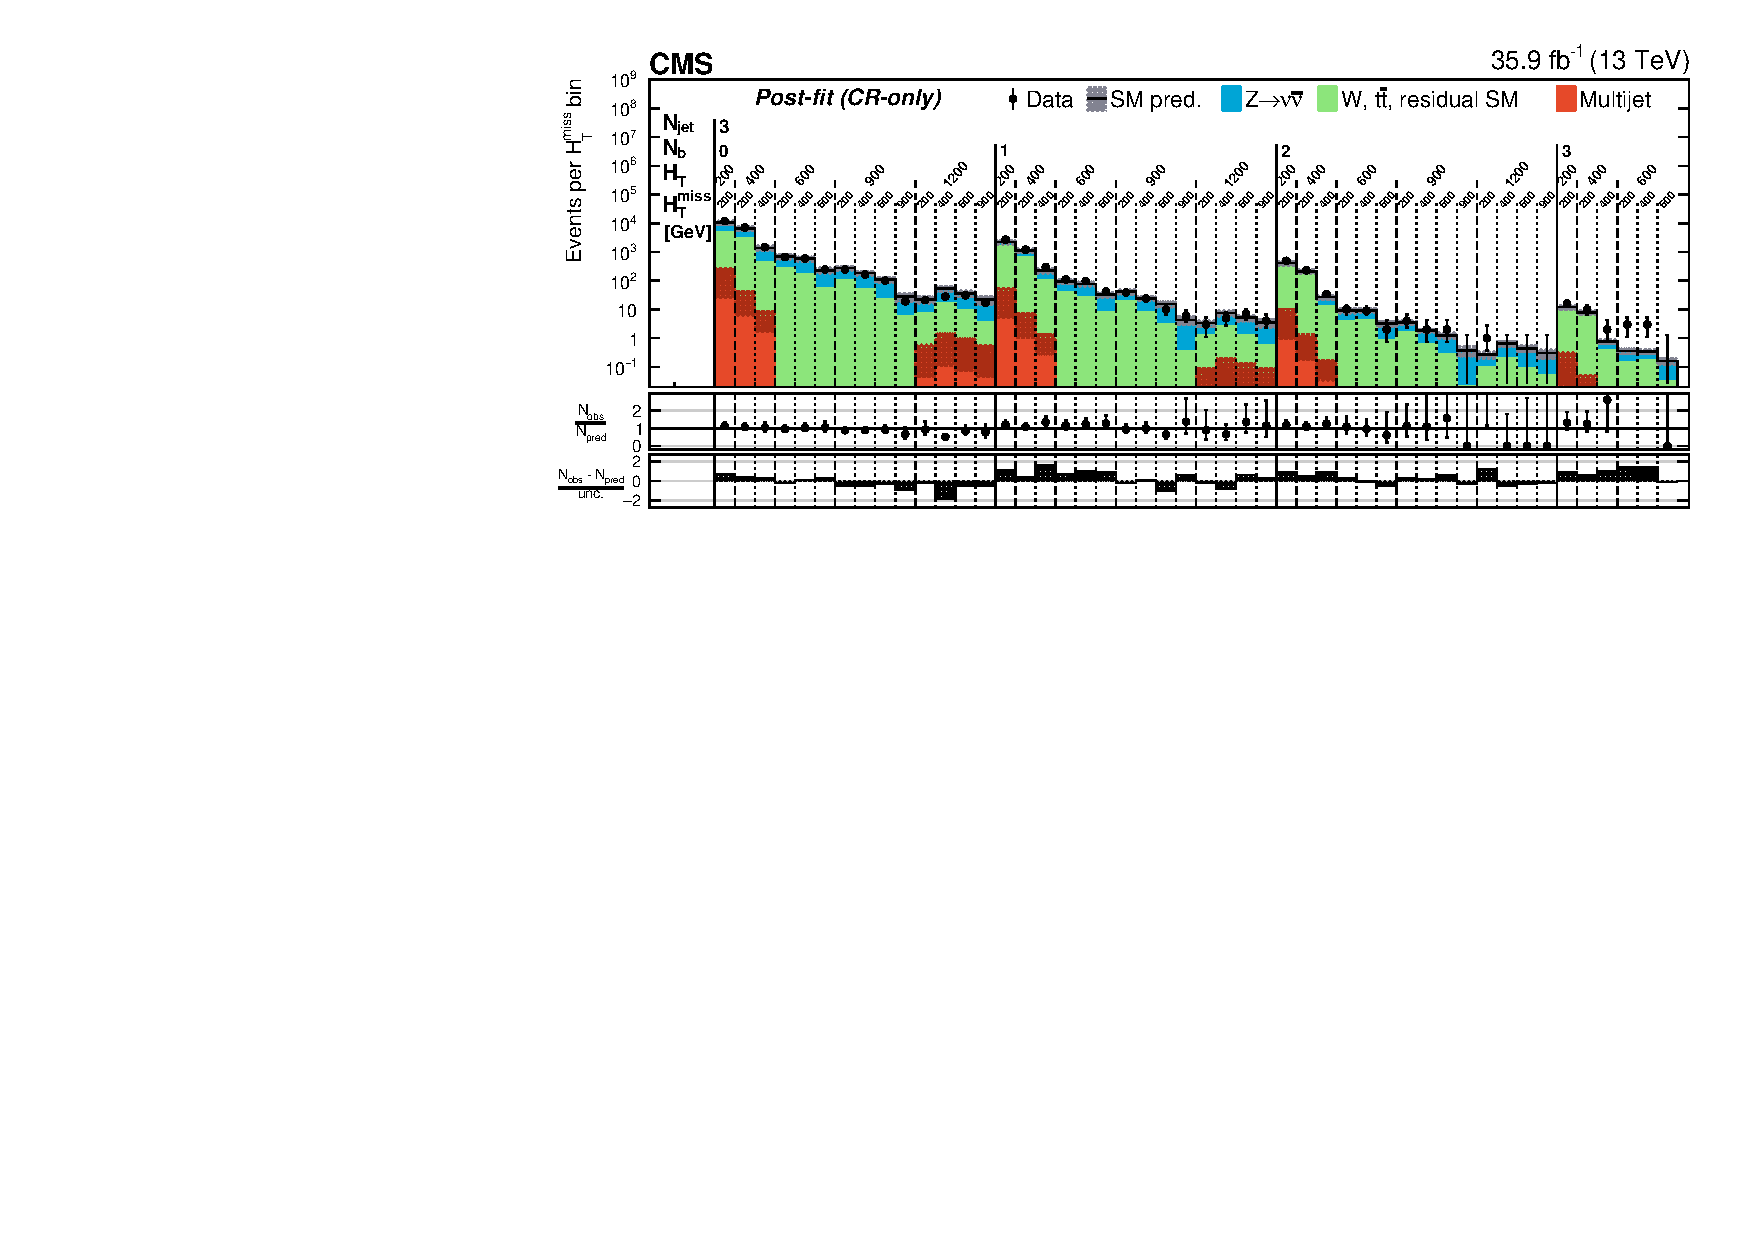
\includegraphics[width=0.99\textwidth, trim=0 0 0 0, 
clip=true]{figs/results/3jet_cr-only.pdf}\\
\caption{Number of events observed (solid markers) and expected number of Z, 
\ttw and QCD background events (histograms, with shaded bands representing the 
statistical and systematic uncertainties) in every \nb, \scalht and \mht bin of 
the jet categories $\njet = 1, \ge2a$ (top), $\njet=2$ (middle), and $\njet=3$ 
(bottom), as determined from the maximum likelihood fit to the control regions. 
The centre panel of each sub-figure shows the ratios of the observed and 
expected counts, while the lower panel shows the corresponding z-score, as 
defined in the text.}
\label{fig:results1}
\end{figure}

\begin{figure}[!p]
\centering
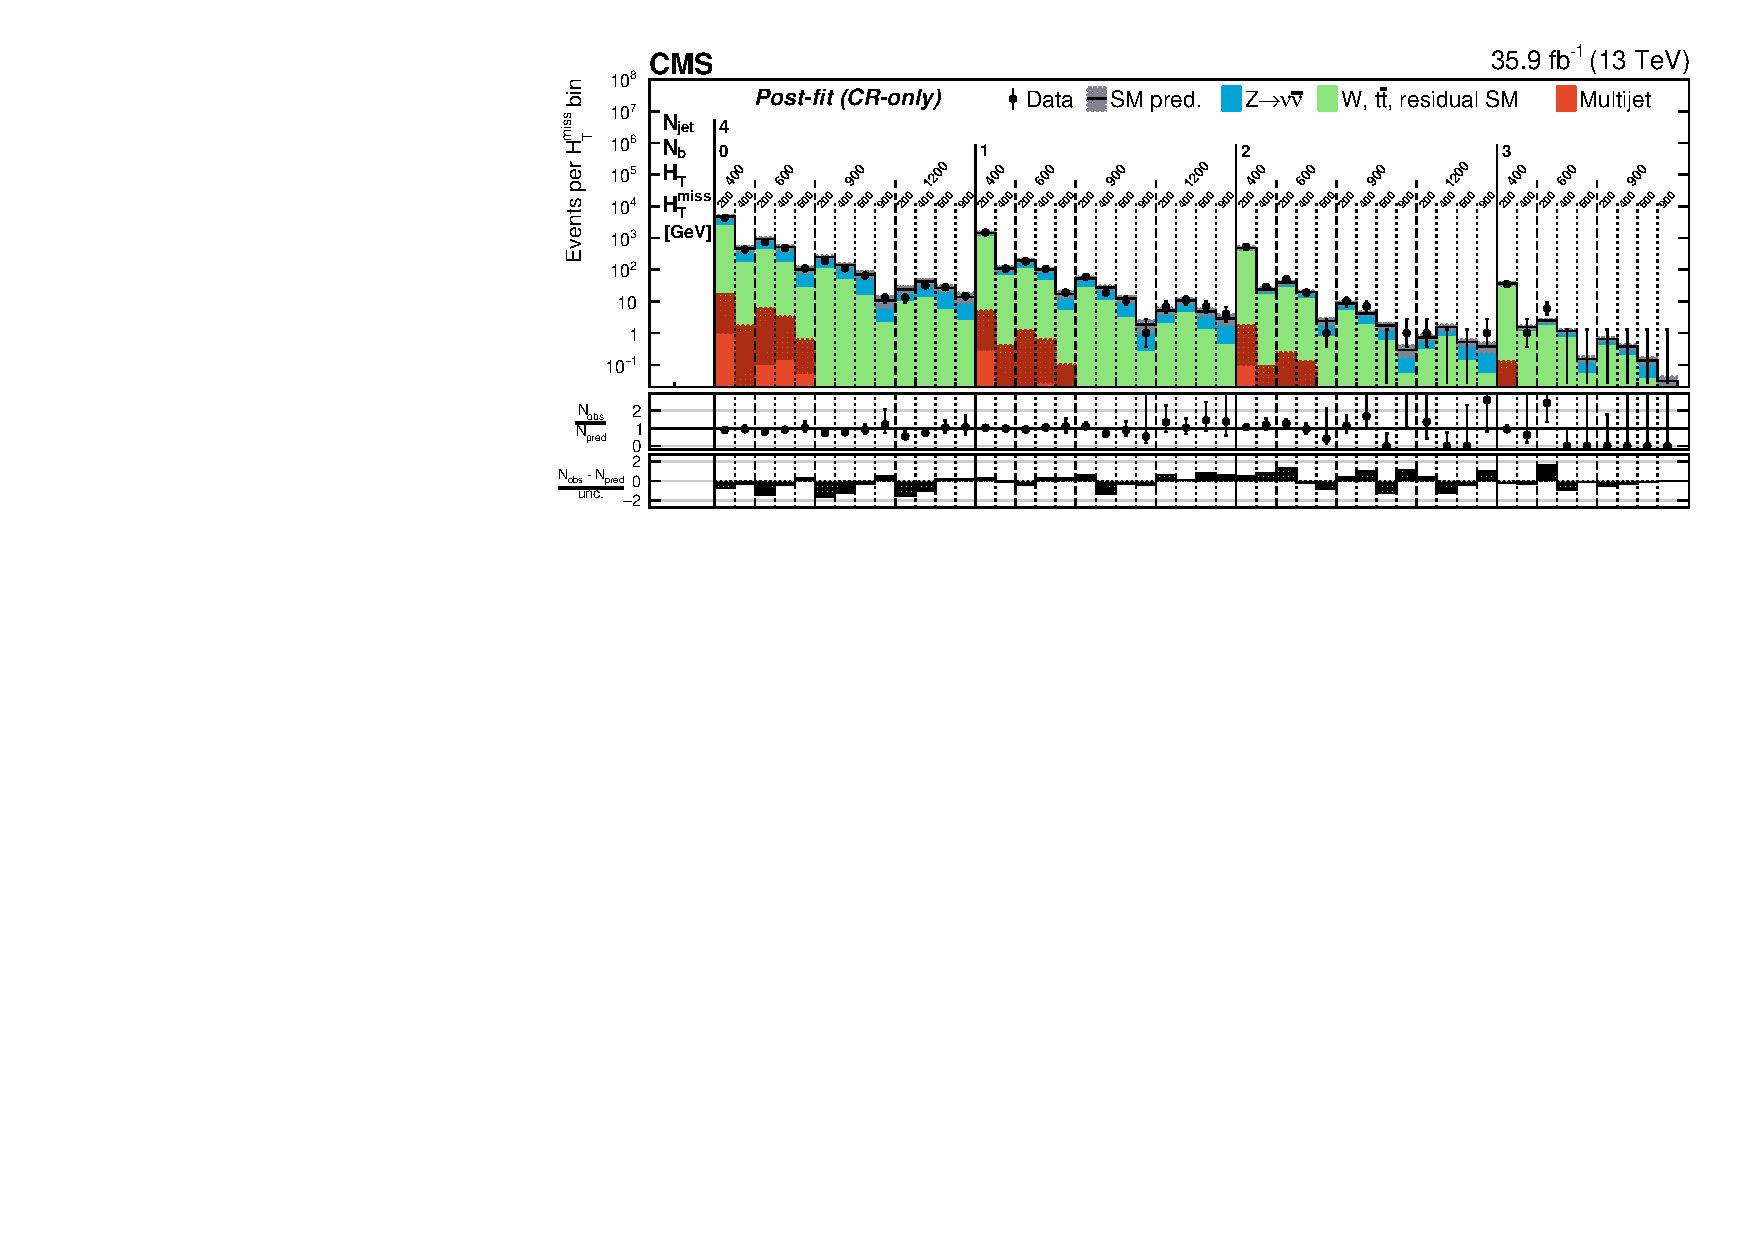
\includegraphics[width=0.99\textwidth, trim=0 0 0 0, 
clip=true]{figs/results/4jet_cr-only.pdf}\\
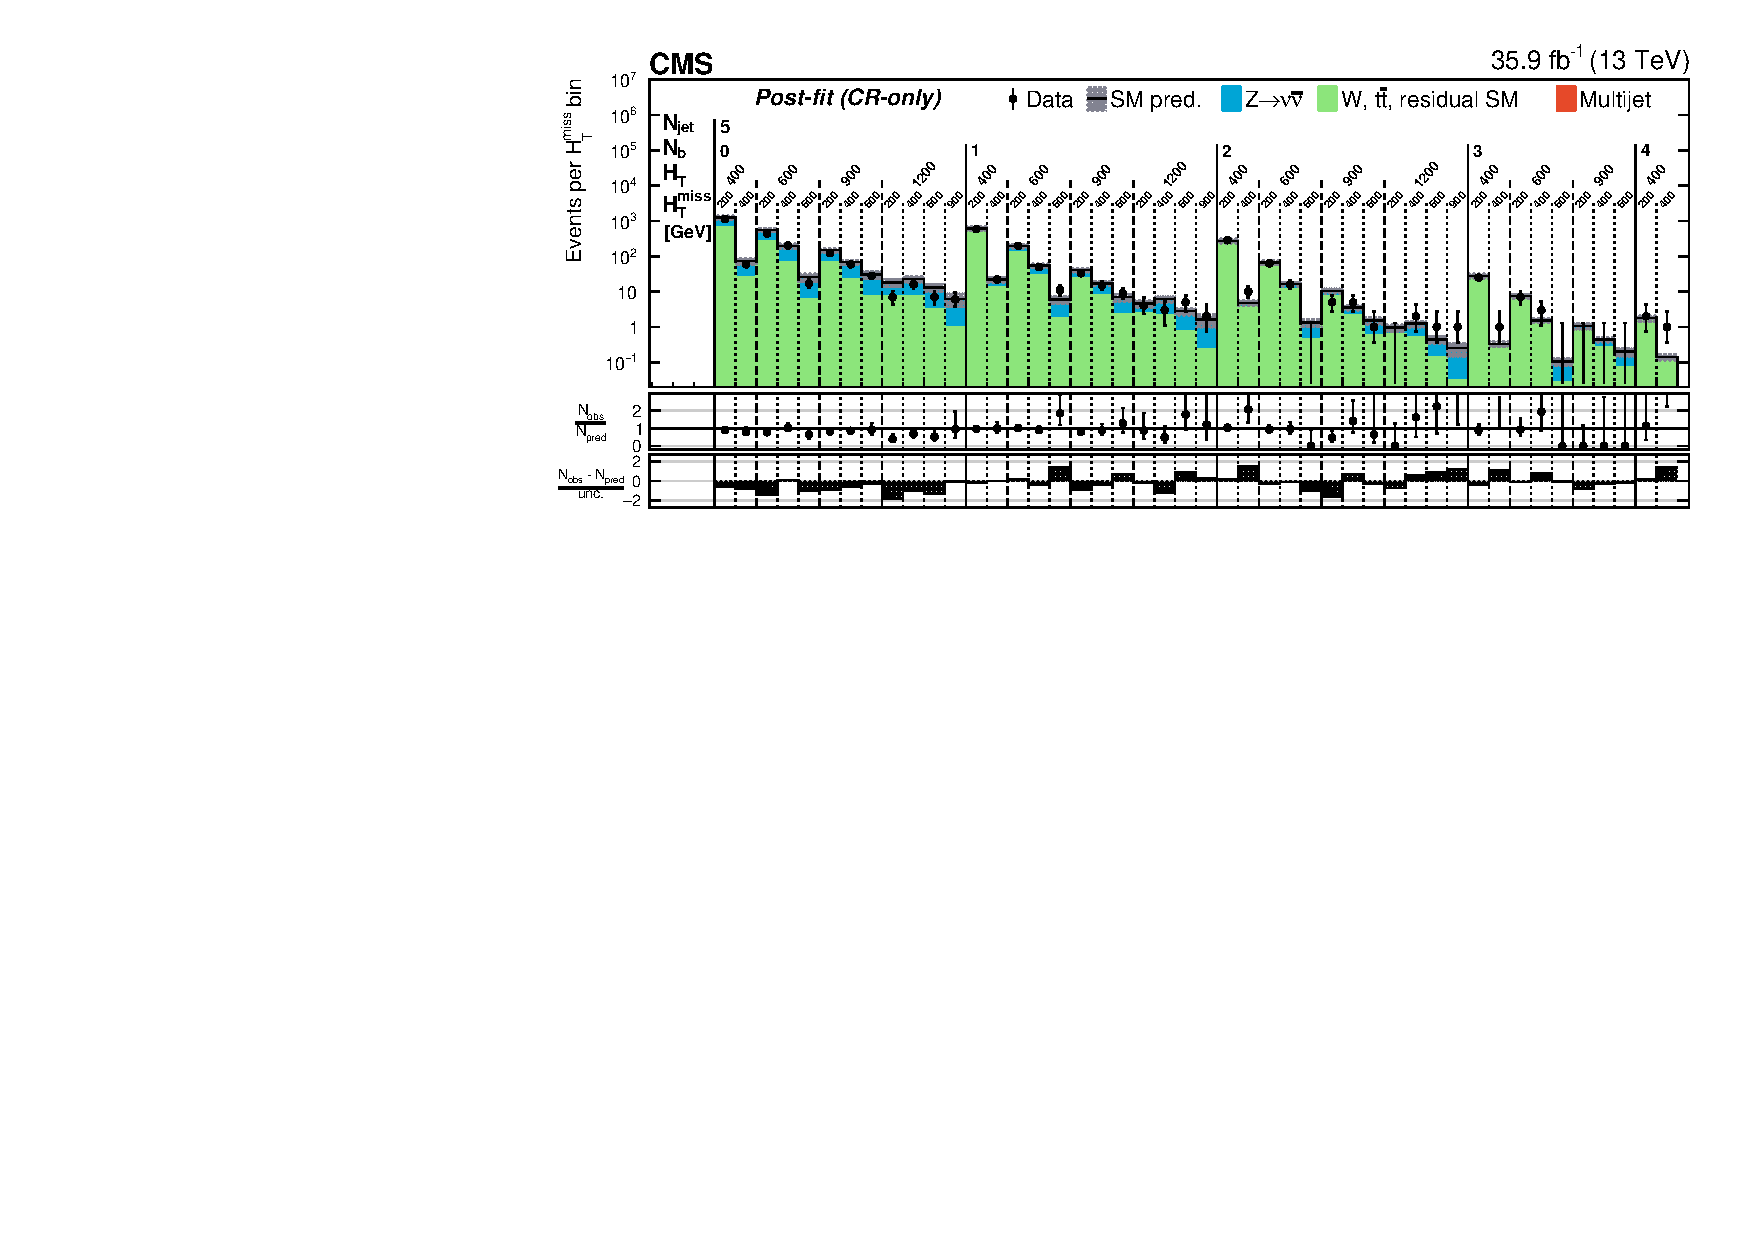
\includegraphics[width=0.99\textwidth, trim=0 0 0 0, 
clip=true]{figs/results/5jet_cr-only.pdf}\\
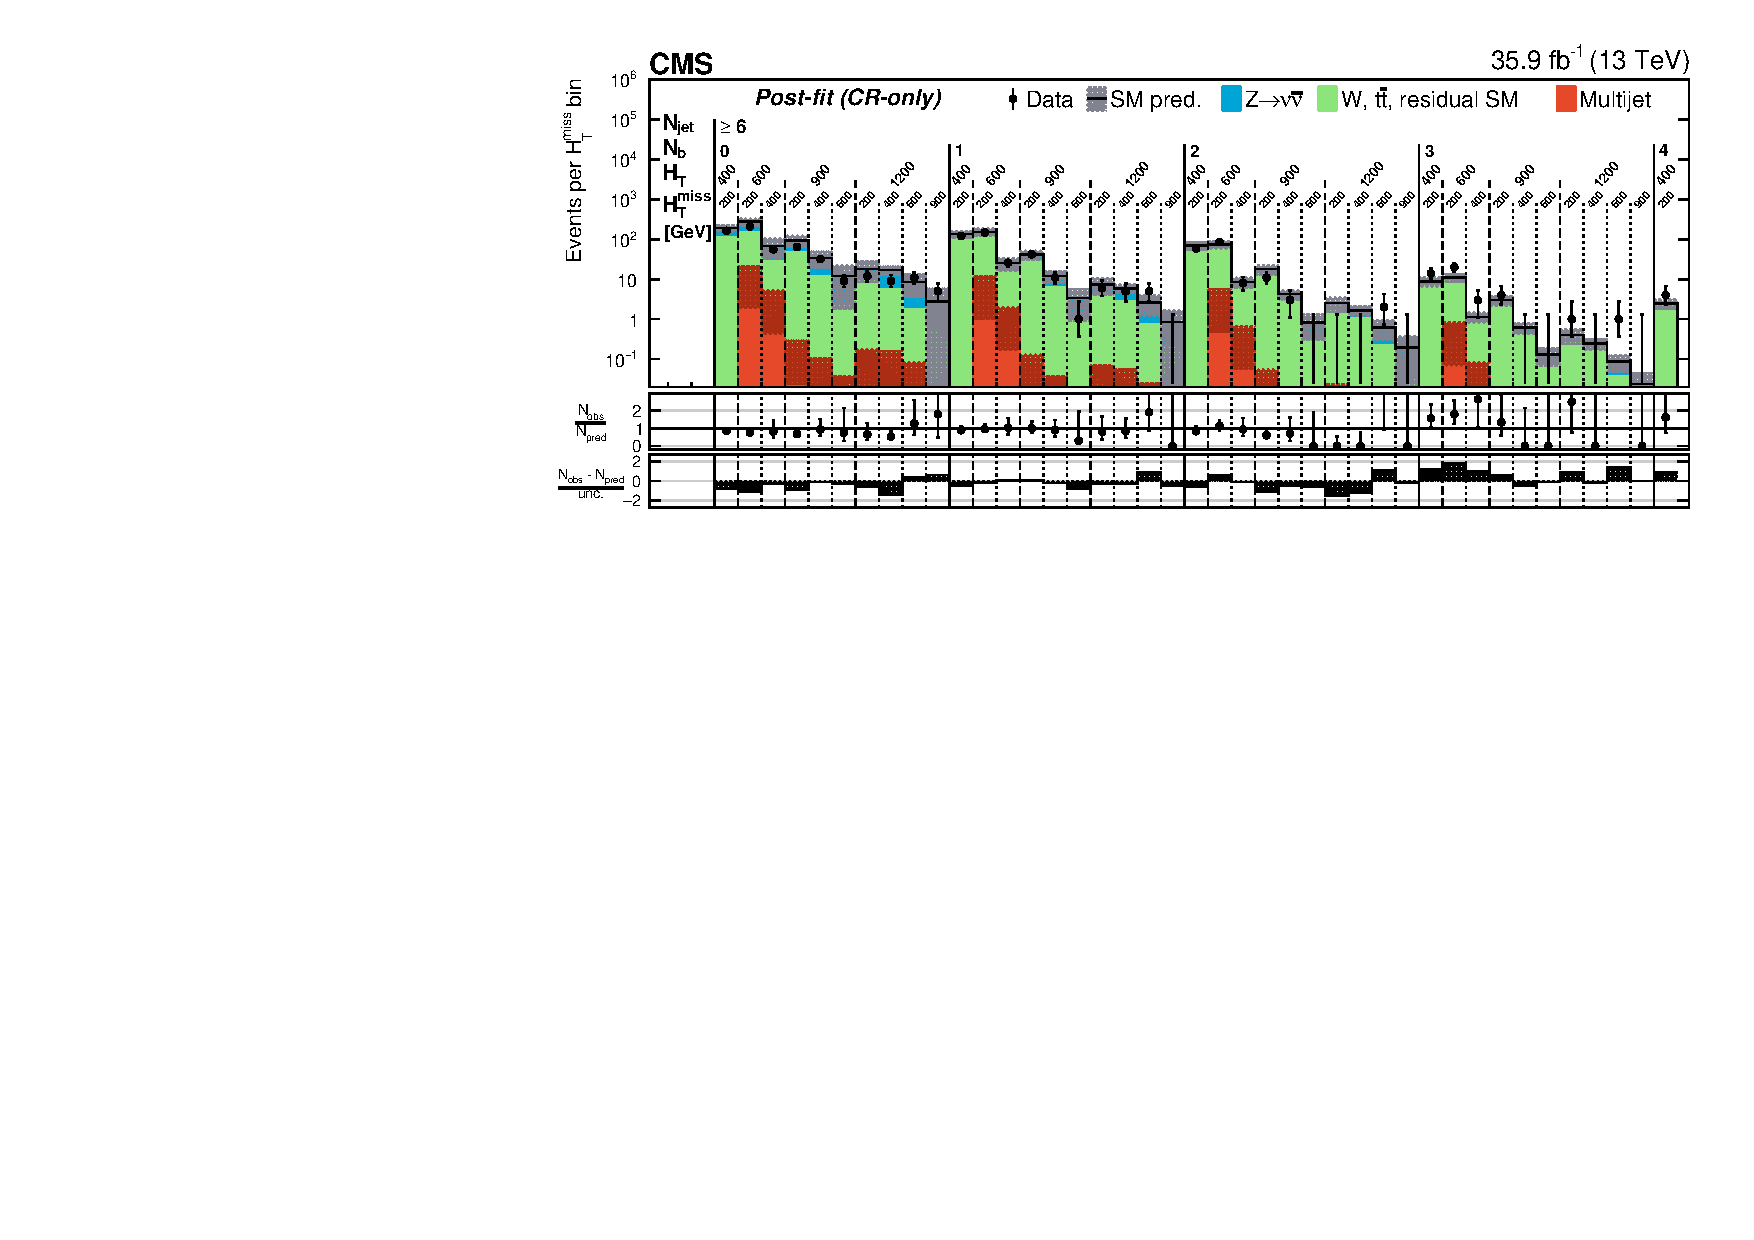
\includegraphics[width=0.99\textwidth, trim=0 0 0 0, 
clip=true]{figs/results/6jet_cr-only.pdf}\\
\caption{Number of events observed (solid markers) and expected number of Z, 
\ttw and QCD background events (histograms, with shaded bands representing the 
statistical and systematic uncertainties) in every \nb, \scalht and \mht bin of 
the jet categories $\njet = 4$ (top), $\njet=5$ (middle), and $\njet\ge6$ 
(bottom), as determined from the background-only maximum likelihood fit to the 
control regions. 
The centre panel of each sub-figure shows the ratios of the observed and 
expected counts, while the lower panel shows the corresponding z-score, as 
defined in the text.}
\label{fig:results2}
\end{figure}

\begin{figure}[h!]
\centering
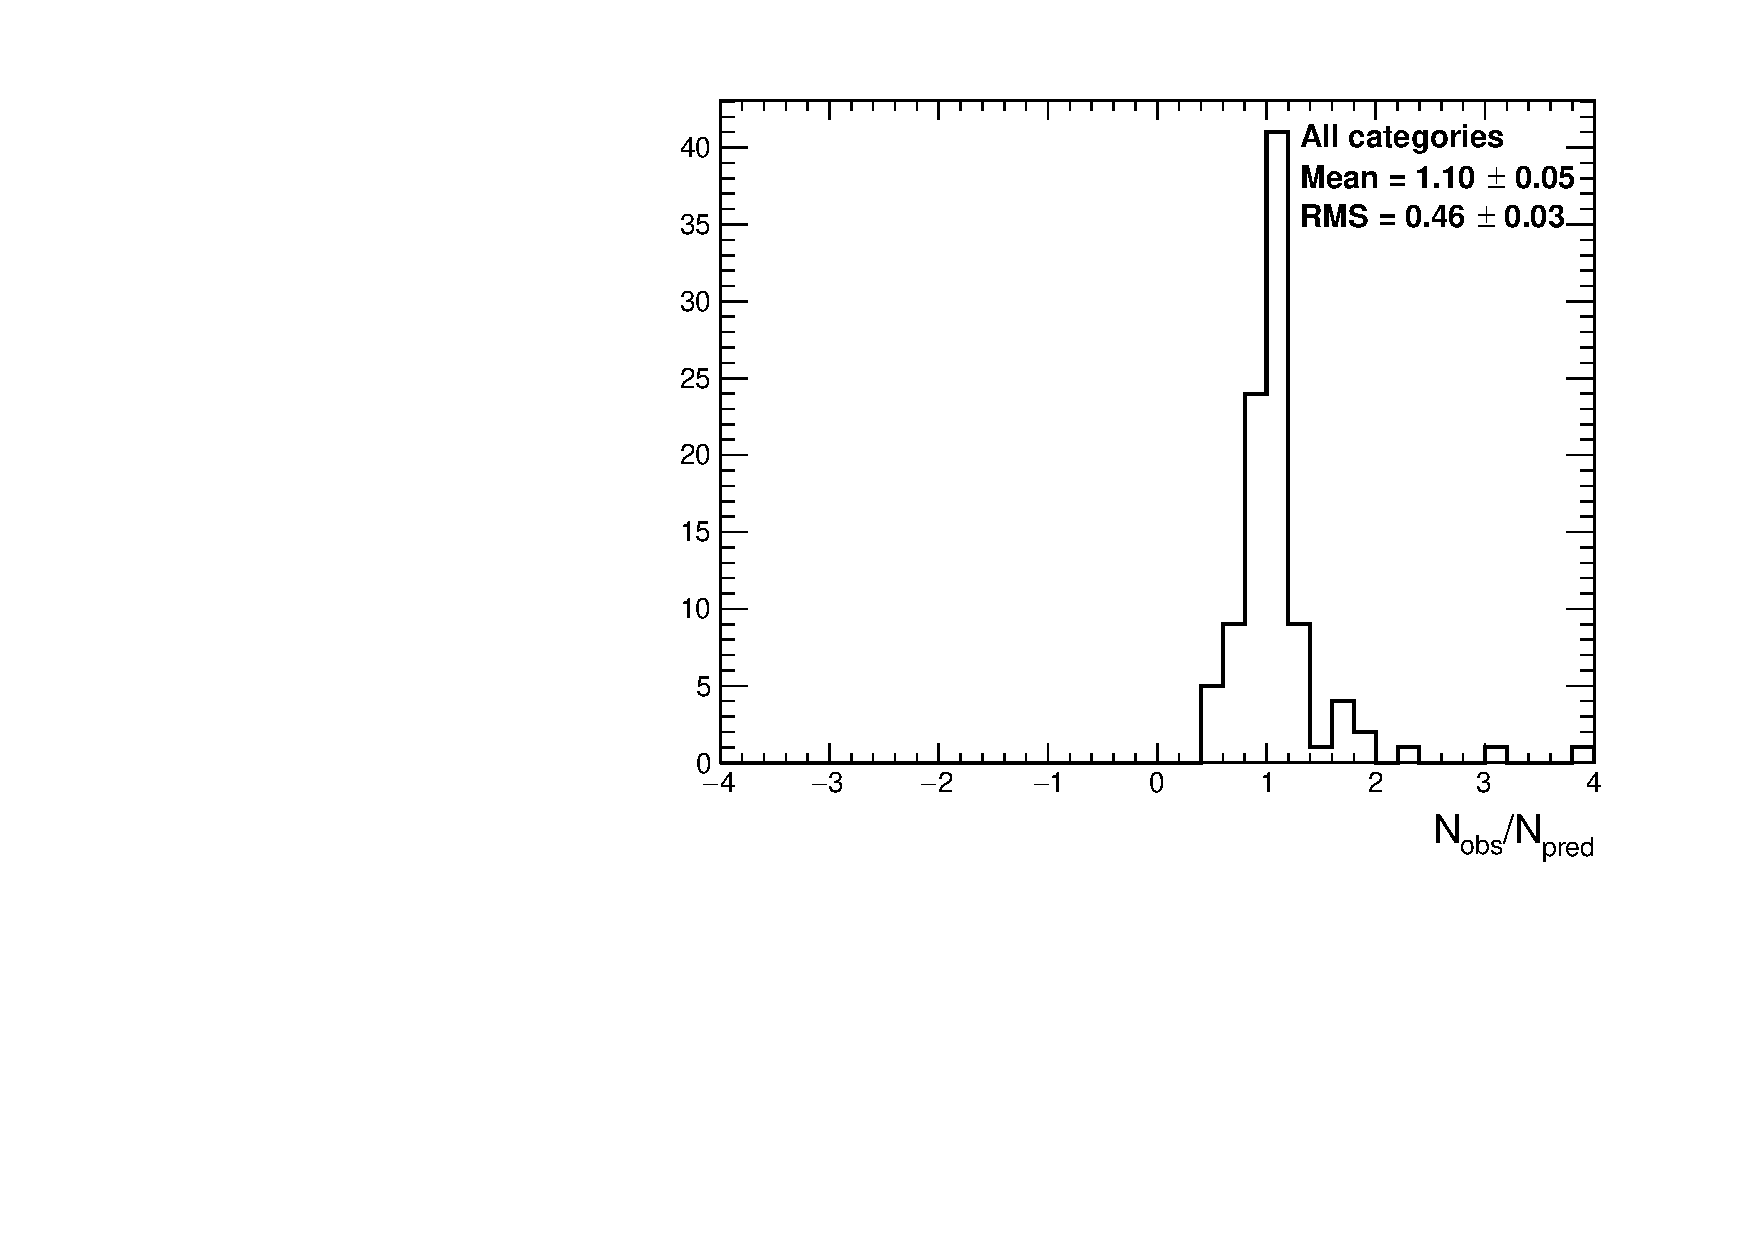
\includegraphics[width=0.49\linewidth]{figs/results/ratios_all_prefit.pdf}
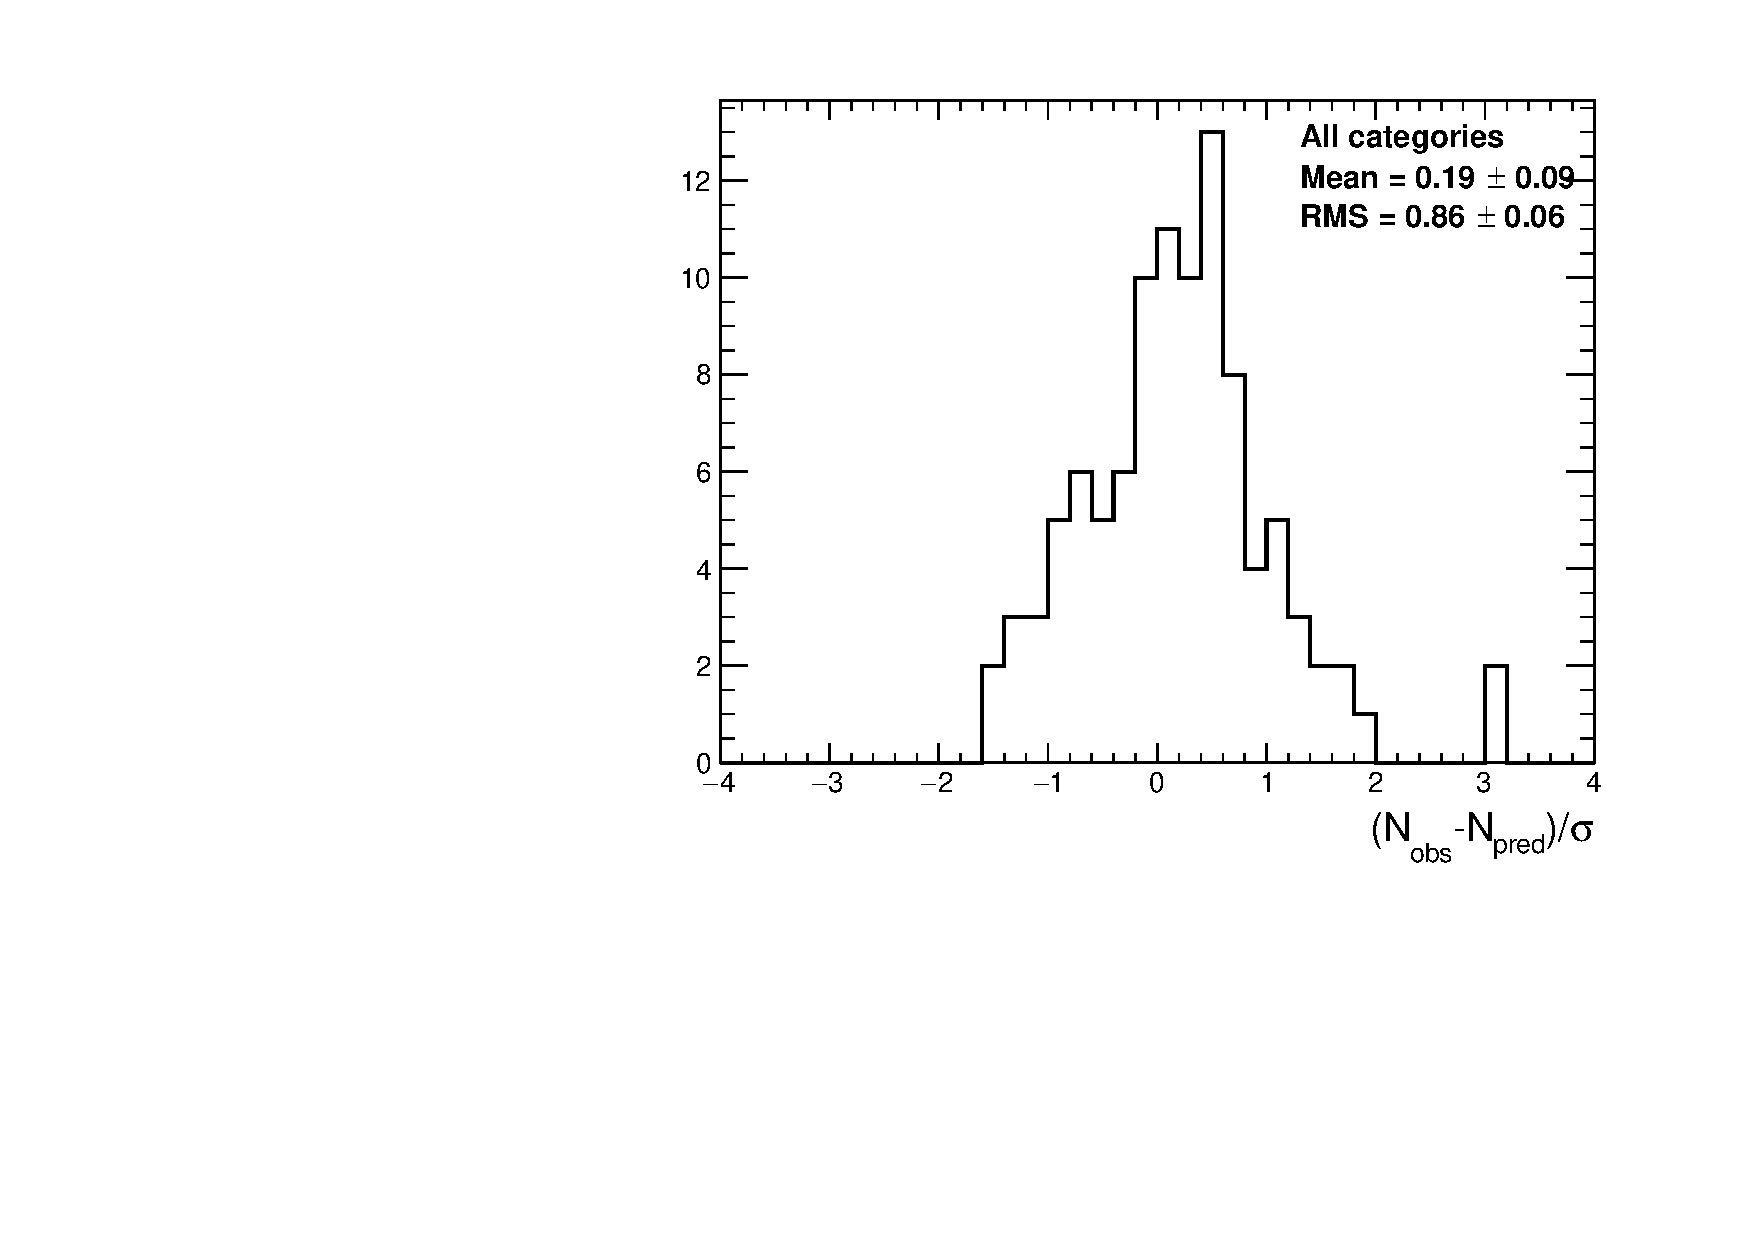
\includegraphics[width=0.49\linewidth]{figs/results/pulls_all_prefit.pdf}
\caption{Histograms of the ratios of the observed and expected event counts 
(left) and corresponding z-scores (right), as defined in the text, for all 
\njnbht bins, as determined from the background-only maximum likelihood fit to 
the control regions.}
\label{fig:ratios_and_pulls}
\end{figure}

\section{Procedure for setting limits on signal models}
%2-3 pages.
\label{sec:results-limitsproc}
Given the good agreement between the observed data and the standard model 
expectation, with no significant excess above the number of expected events in 
any bin, no evidence of new physics beyond the standard model is found. 
Statistical hypothesis tests are carried out in order to assess the 
incompatibility of the data with various models of long-lived supersymmetry. 
Upper bounds are placed on their cross sections at a 95\% confidence level.
%Upper limits 
%exclusion
%Given no excess, set limits.
%Hypothesis testing, setting limits, asymptotic CLs
%See Nick.

In the hypothesis tests, the parameter being tested is the signal strength, 
while all other parameters are considered to be nuisance parameters, labelled 
collectively as $\bm{\theta}$.
For a test of a model with a signal strength of $\mu_s$, one can use a profile 
likelihood ratio as a test statistic:
\begin{equation}
t(\mu_s) = 2 \ln \frac{\mathcal{L}(\hat{\mu}_s, 
\hat{\bm{\theta}})}{\mathcal{L}(\mu_s, \hat{\bm{\theta}}(\mu_s))}
\end{equation}
where $\hat{\mu}_s$ and $\hat{\bm{\theta}}$ are the global maximum likelihood 
values of the signal strength 
and nuisance parameters, and $\hat{\bm{\theta}}(\mu_s)$ is the maximum 
likelihood value of the nuisance 
parameters for a fixed signal strength of $\mu_s$. 
%The numerator of the ratio is the largest possible value of the likelihood 
%function
%denominator of the ratio is, by definition, not larger than the numerator. 
A value of $t(\mu_s)=0$ represents a perfect agreement between the hypothesised 
signal strength $\mu_s$ and the observed data, while larger values of 
$t(\mu_s)$ represent an increasing incompatibility between $\mu_s$ and the data.

The best fit value of the signal strength is constrained to lie within $0 \le 
\hat{\mu}_s \le \mu_s$. The lower constraint is imposed so as to avoid a  
non-physical cross section. The upper bound is chosen so that an upward 
fluctuation in the signal counts such that $\hat{\mu}_s > \mu_s$ is not treated 
as evidence against that model. 
%also so one-sided bound/limit
The final test statistic is then given by~\cite{higgscombine}:
\begin{equation}
t(\mu_s) = 
	\begin{cases}
	2 \ln \frac{\mathcal{L}(0, \hat{\bm{\theta}}(0))}{\mathcal{L}(\mu_s, 
	\hat{\bm{\theta}}(\mu_s))} & \hat{\mu}_s < 0 \\
	2 \ln \frac{\mathcal{L}(\hat{\mu}_s, \hat{\bm{\theta}})}{\mathcal{L}(\mu_s, 
	\hat{\bm{\theta}}(\mu_s))} & 0 \le \hat{\mu}_s \le \mu_s \\
	0 & \hat{\mu}_s > \mu_s
	\end{cases}
\end{equation}

The incompatibility of a signal model with data can be assessed with the 
p-value:
\begin{equation}
\mathrm{CL}_{b+s}(\mu_s) = \int_{t(\mu_s)_{\mathrm{obs}}}^{\infty} 
f(t(\mu_s)|\mu_s) \mathrm{d}t(\mu_s)
\end{equation}
where $f(t(\mu_s)|\mu_s)$ is the probability density of the test statistic 
under the hypothesised signal strength $\mu_s$, and $t(\mu_s)_{\mathrm{obs}}$ 
is 
the value of the test statistic observed in 
data. In order to reject a signal model, not only is a small p-value 
$\mathrm{CL}_{b+s}$ 
required, but also a good compatibility with the background-only model, as 
determined by the probability:
\begin{equation}
\mathrm{CL}_{b}(\mu_s) = \int_{t(\mu_s)_{\mathrm{obs}}}^{\infty} f(t(\mu_s)|0) 
\mathrm{d}t(\mu_s)
\end{equation}
where $f(t(\mu_s)|0)$ is the probability density of the test statistic under 
the background-only model ($\mu_s=0$). The ratio of the two probabilities is 
then constructed as~\cite{cls1,cls2}:
\begin{equation}
\mathrm{CL}_s(\mu_s) = \frac{\mathrm{CL}_{b+s}(\mu_s)}{\mathrm{CL}_{b}(\mu_s)}
\end{equation}
%CLs which is designed to provide less stringent exclusion limits in analyses 
%which are less sensitive to signal [69]. (think S and B distrs very similar)
A particular signal strength is considered to be excluded at a 95\% confidence 
level if the corresponding $\mathrm{CL}_s$ value is less than 0.05. For a given 
signal model, the upper limit on the signal strength $\mu_s^{95\%}$ is given by 
the largest value of $\mu_s$ that is excluded with $\mathrm{CL}_s<0.05$. 

The distributions $f(t(\mu_s)|\mu_s)$ and $f(t(\mu_s)|0)$ are approximated by 
analytical probability 
functions that are derived in the limit of a large sample of 
events~\cite{asymptotic-formulae}. 
While the above procedure provides the \textit{observed} limit on the signal 
strength, an \textit{expected} limit can also be computed as the median value 
of $\mu_s^{95\%}$ obtained under the background-only model. The uncertainty on 
the expected limit is given by the appropriate quantiles of the distribution of 
$\mu_s^{95\%}$.
%expected limit (mu=0), find mu such that median (16,84,etc) 
%asymptotic vs toys

%background-only hypothesis ($\mu_s=0$) and the background-plus-signal 
%hypothesis ($\mu_s \ne 0$)


\section{Limits on long-lived supersymmetry}
\label{sec:results-limits}
%consider LL gluino model (reference simplified model section in theory 
%chapter), don't call it t1qqqqll
%set limits in mass plane for various ctau - for each mass calculate mu limit, 
%then exclusion contours are where mu=1.
Simplified models of Split SUSY are simulated with a range of gluino and LSP 
masses for various gluino lifetimes from $1~\micro\metre$ to 100~m, in addition 
to a 
promptly decaying and metastable gluino. An upper limit on the signal strength 
(and cross section) of each model is computed. These limits are presented in 
the ($\mglu$, $\mlsp$) plane for each simulated value of $\ctau$ in 
Figs.~\ref{fig:limits-individual-1}~-~\ref{fig:limits-individual-3}.
The excluded regions correspond to mass points with limits on their signal 
strength of $\mu_s^{95\%} < 1$. 
Both the expected and observed excluded regions are shown, with experimental 
uncertainties and uncertainties on the theoretical cross sections indicated. 
The excluded mass regions for each value of $\ctau$ are summarised in 
Fig.~\ref{fig:limits-summary}.
%summarise highest excluded mass in table?

%all 11 individual limit plots.
%shown with 1 and 2 sigma experimental uncertainties on expected, and 
%theoretical uncertainty on observed (what is this?)
%The band around the expected 1883 exclusion reflects the experimental 
%%%uncertainty, while the band around the observed exclusion 1884 correspond to 
%%%%the theoretical uncertainty on the signal cross section.
%then one summary plot (maybe just observed contours).
%ctau-mass limit plane?

For the model with a promptly decaying gluino, gluino and LSP masses of up to 
$\sim$1650~GeV and $\sim$900~GeV, respectively, are excluded. The excluded 
regions for models with gluino lifetimes of $\ctau = 1, 10, 100~\micro\metre$ 
are comparable to the prompt decay scenario. 
A moderate improvement in sensitivity is found for models with $\ctau = 1, 
10$~mm, with maximum excluded gluino and LSP masses of 1750~GeV and 1000~GeV, 
respectively. This is because these signal events occupy the high \nb 
categories, and the amount of background is considerably smaller than in the 
bins with no b-tagged jets. 
The sensitivity is reduced for models with lifetimes larger than $\ctau > 
100$~mm as the acceptance to jets from the gluino decay becomes smaller. The 
limiting case is that of a metastable gluino. In this case, the gluinos always 
decay outside of the detector and so the acceptance for these models relies 
entirely on ISR jets. Gluino masses up to 900~GeV are excluded, and the 
sensitivity is independent of the LSP mass.
%explain pattern in limits (line 538 in paper) prompt-low-med-high-stable ctau.
%1 mm improvement because less background in high nb bins 
%less background in high nj/nb.
%mention which are MSBs (no need for plots), refer back to yield plots.

%FIXME
%Mention 2sigma excess (refer back to results) (line 531)
%fluctuations mostly nb>=1 and monojet
The observed exclusion regions are found to be $\sim$1-2$\sigma$ weaker than 
the expected ones for most of the models considered. This difference is due to 
slight upward fluctuations in the observed events across several categories in 
the signal region.
%in particular in the $\nb \ge 1$ categories. 
%\textbf{This suggests we are close to confirming the existence of 
%%%supersymmetry. In particular, it seems that SUSY exists in a superposition 
%%%of all possible masses and lifetimes.}

%(line 550 in paper)
%say r-hadron interaction model can be of varied forms. For simplicity here 
%don't simulate interactions, but the effect has been checked for couple of 
%pball models - negligible except for large lifetimes when get muons and 
%isolated tracks and limits degrade by only 50-100 GeV.
As mentioned in Sec.~\ref{sec:analysis-samples-mc}, the results for the Split 
SUSY models have been obtained assuming no interactions of the R-hadrons with 
the detector material. Nevertheless, the effect of matter interactions has been 
checked. A 
non-negligible fraction of R-hadrons that traverse the muon chambers 
are identified as muons. Similarly, charged R-hadrons that decay near the 
calorimeters may be reconstructed as single isolated tracks. This leads to a 
reduction in acceptance for models with $\ctau \gtrsim 1$~m as a consequence of 
the veto on events containing muons or isolated tracks.
% When simulated using a cloud model of hadronisation 
% When these signal models are simulated using a cloud model and prob  gluino 
%ball 10\%, 
The excluded mass regions weaken by 50-200~GeV for these signal models. The 
change is negligible for models with $\ctau \lesssim 1$~m.

%paper: The search provides coverage that is complementary to other dedicated 
%techniques at the LHC, such as for models with long-lived gluinos with ct0 . 
%1mm.
%to conclude this chapter: good sensitivity, considering it's not a dedicated 
%search, complementary for sub-cm.
%Thanks to inclusiveness/low thresholds have good sensitivity to very-LL.
%complimentarity with dedicated searches? cms stopped and atlas displaced 
%vertices
Despite being optimised for prompt decay signatures and not employing dedicated 
techniques for identifying long-lived particles, the search can be seen to have 
a good sensitivity across a wide range of lifetimes and masses. This is mainly 
due to the inclusive nature of the search, with low thresholds on kinematic 
variables such as \scalht and \njet, and an acceptance to jets from ISR.
% also partly b-tagging
In particular, this search provides coverage that is complementary to dedicated 
searches at the LHC for models with $\ctau \lesssim 1$~cm or a metastable 
gluino, as well as models with a very compressed mass spectrum.
%This is beacause dedicated searches need a minimum decay length;
% if lifetime too long then doesn't decay inside detector or within lhc run
% if compressed can't see decay products
This is because dedicated techniques require a minimum decay length and a decay 
that occurs within the detector and within the time frame of an LHC run, as 
well as a sufficiently large mass difference such that the decay products can 
be reconstructed.

\clearpage
\begin{figure}[!t]
\centering
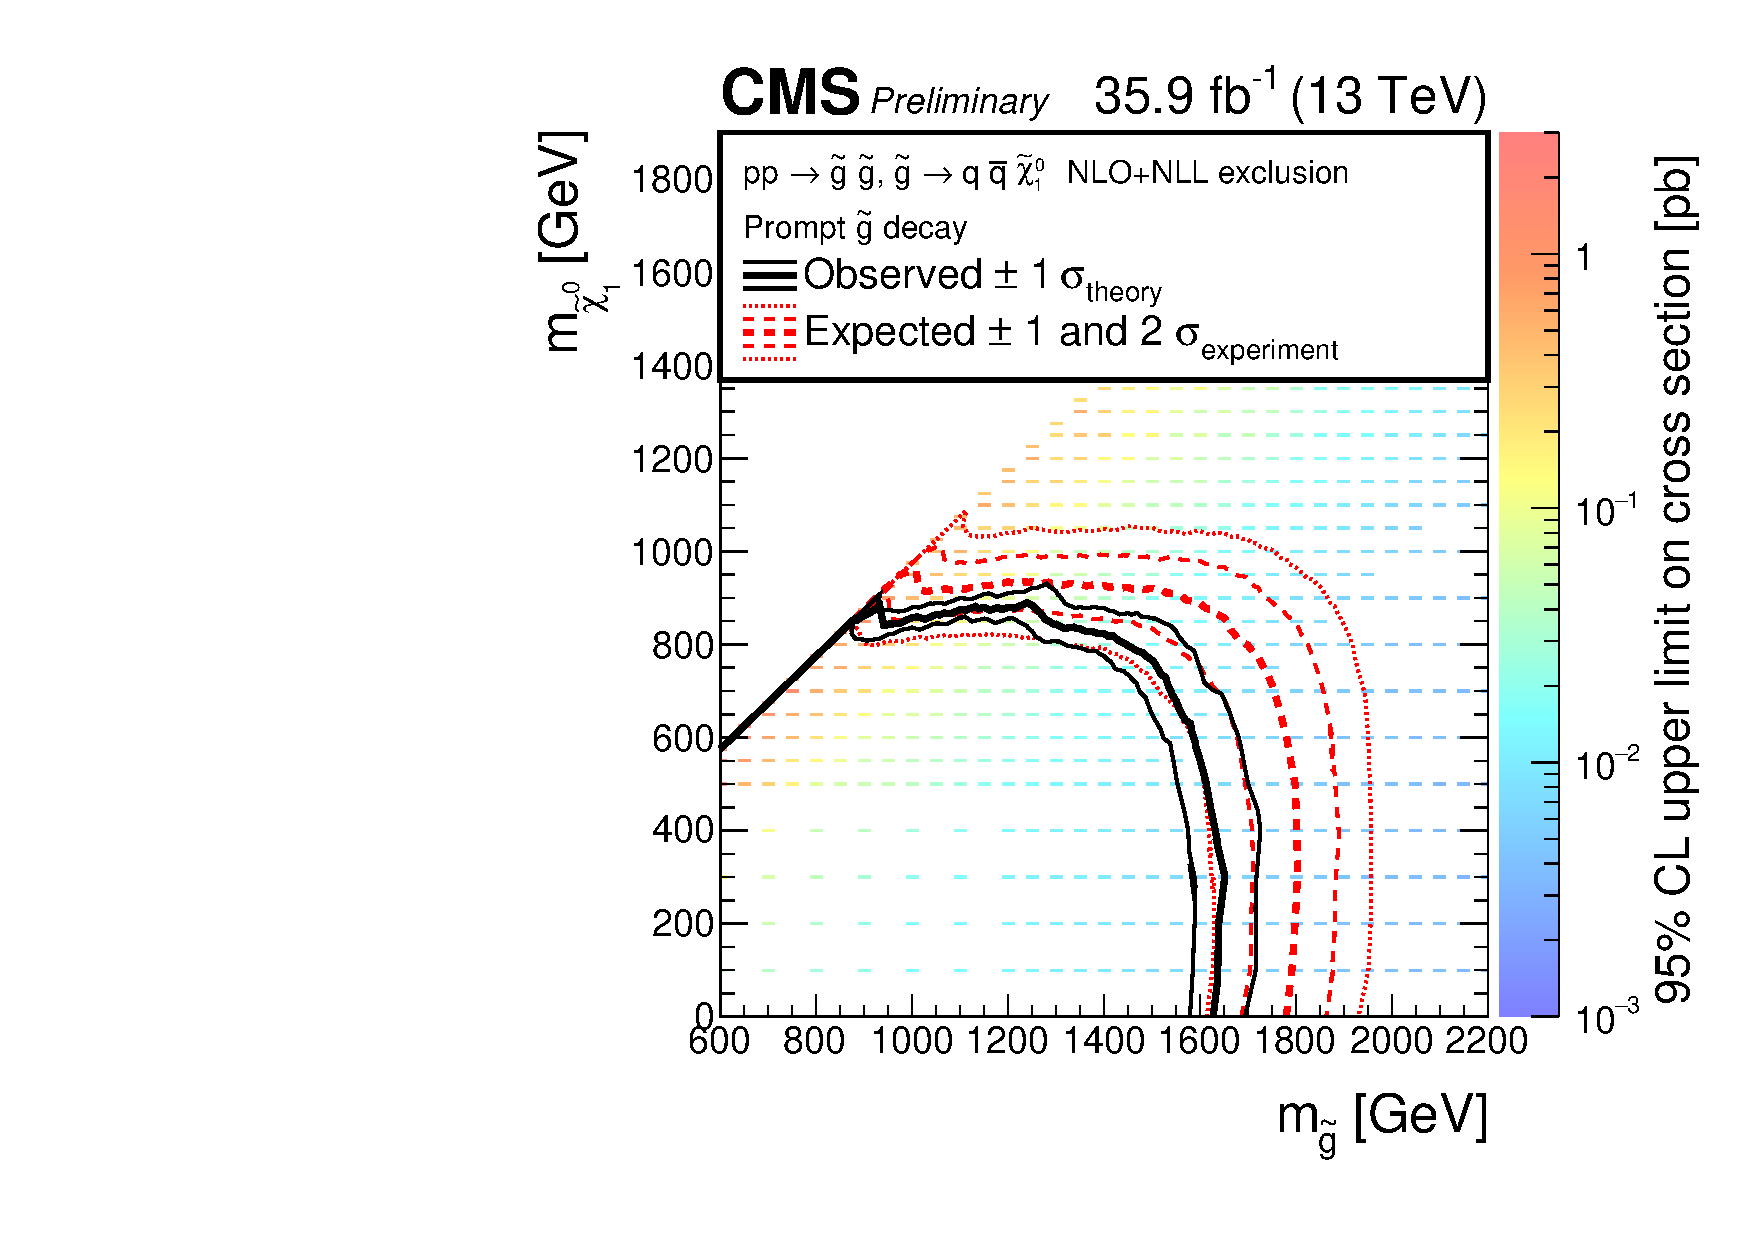
\includegraphics[width=0.49\textwidth]{figs/results/T1qqqqLLPromptXSEC}~
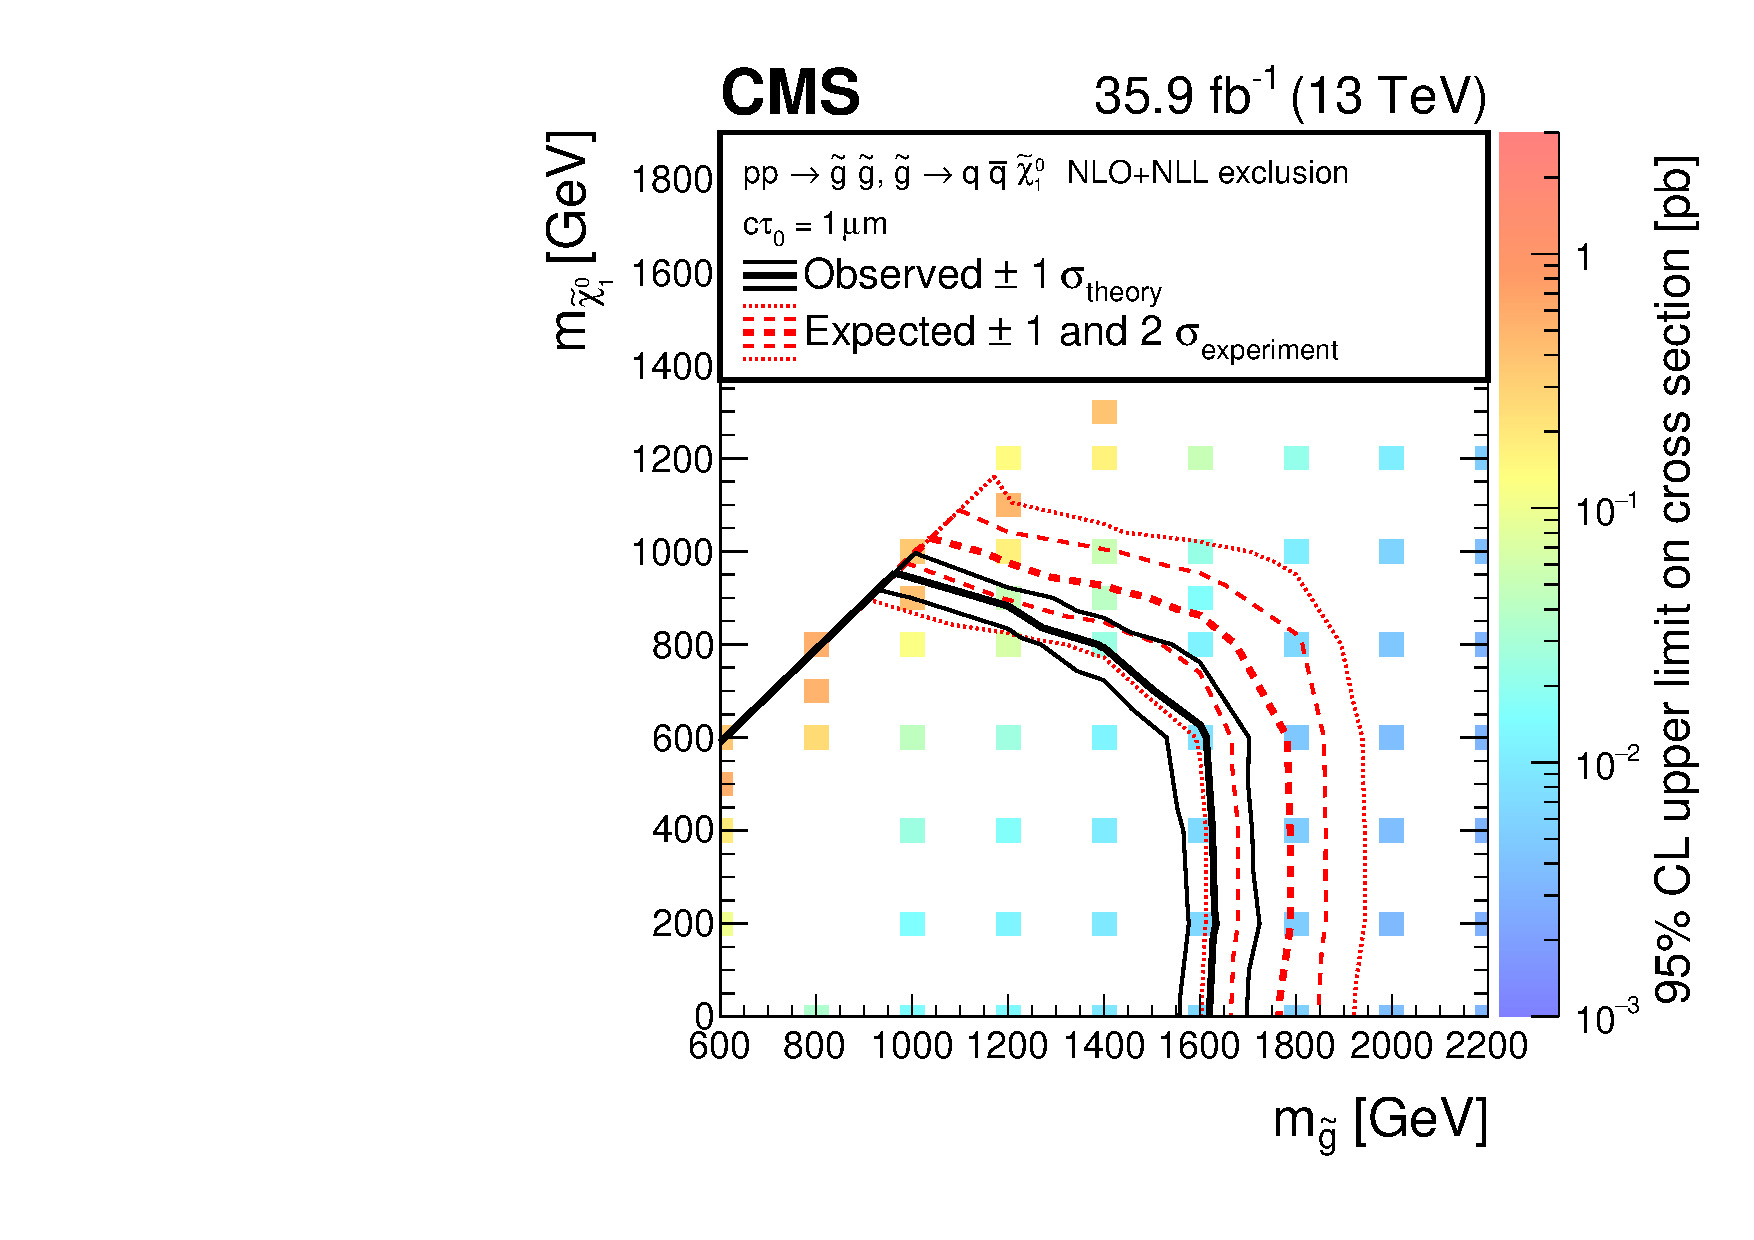
\includegraphics[width=0.49\textwidth]{figs/results/T1qqqqLL0p001XSEC}\\
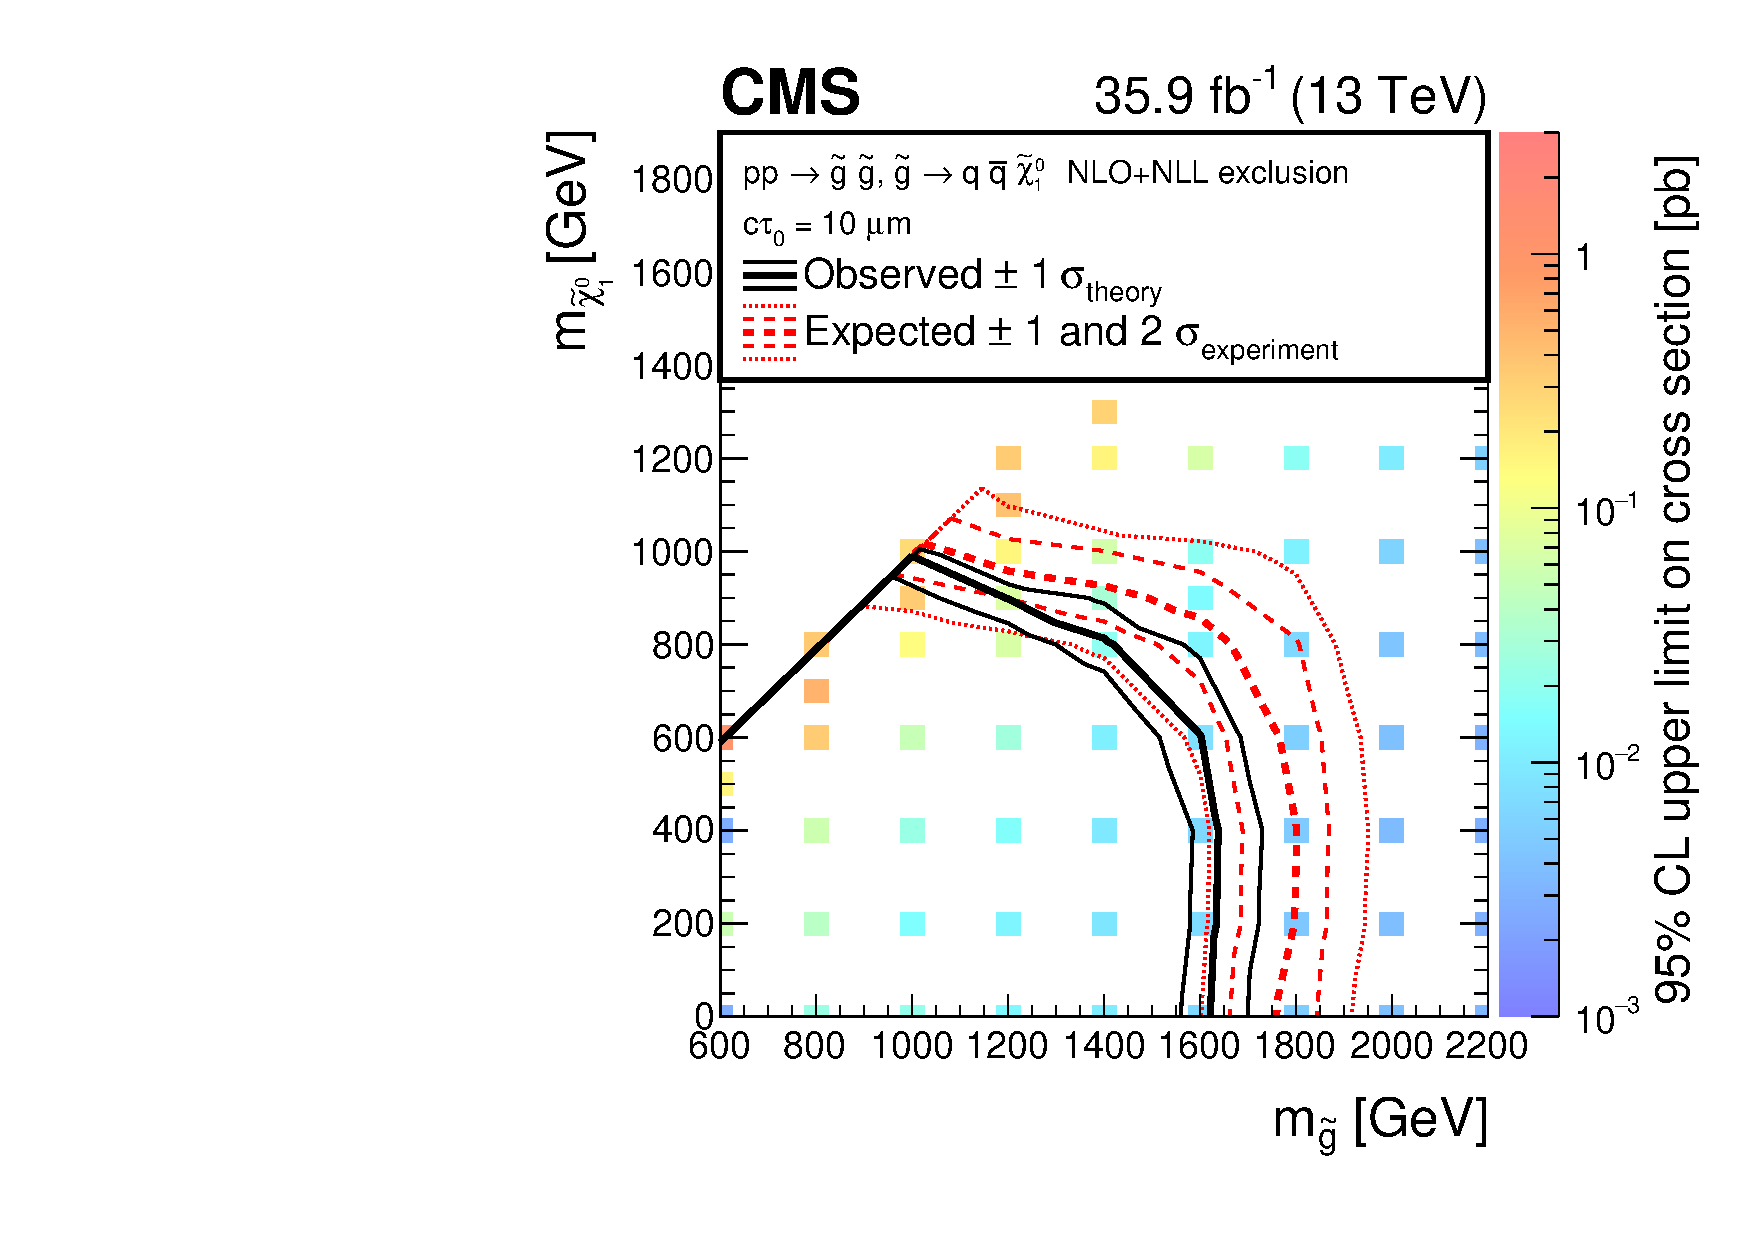
\includegraphics[width=0.49\textwidth]{figs/results/T1qqqqLL0p01XSEC}~
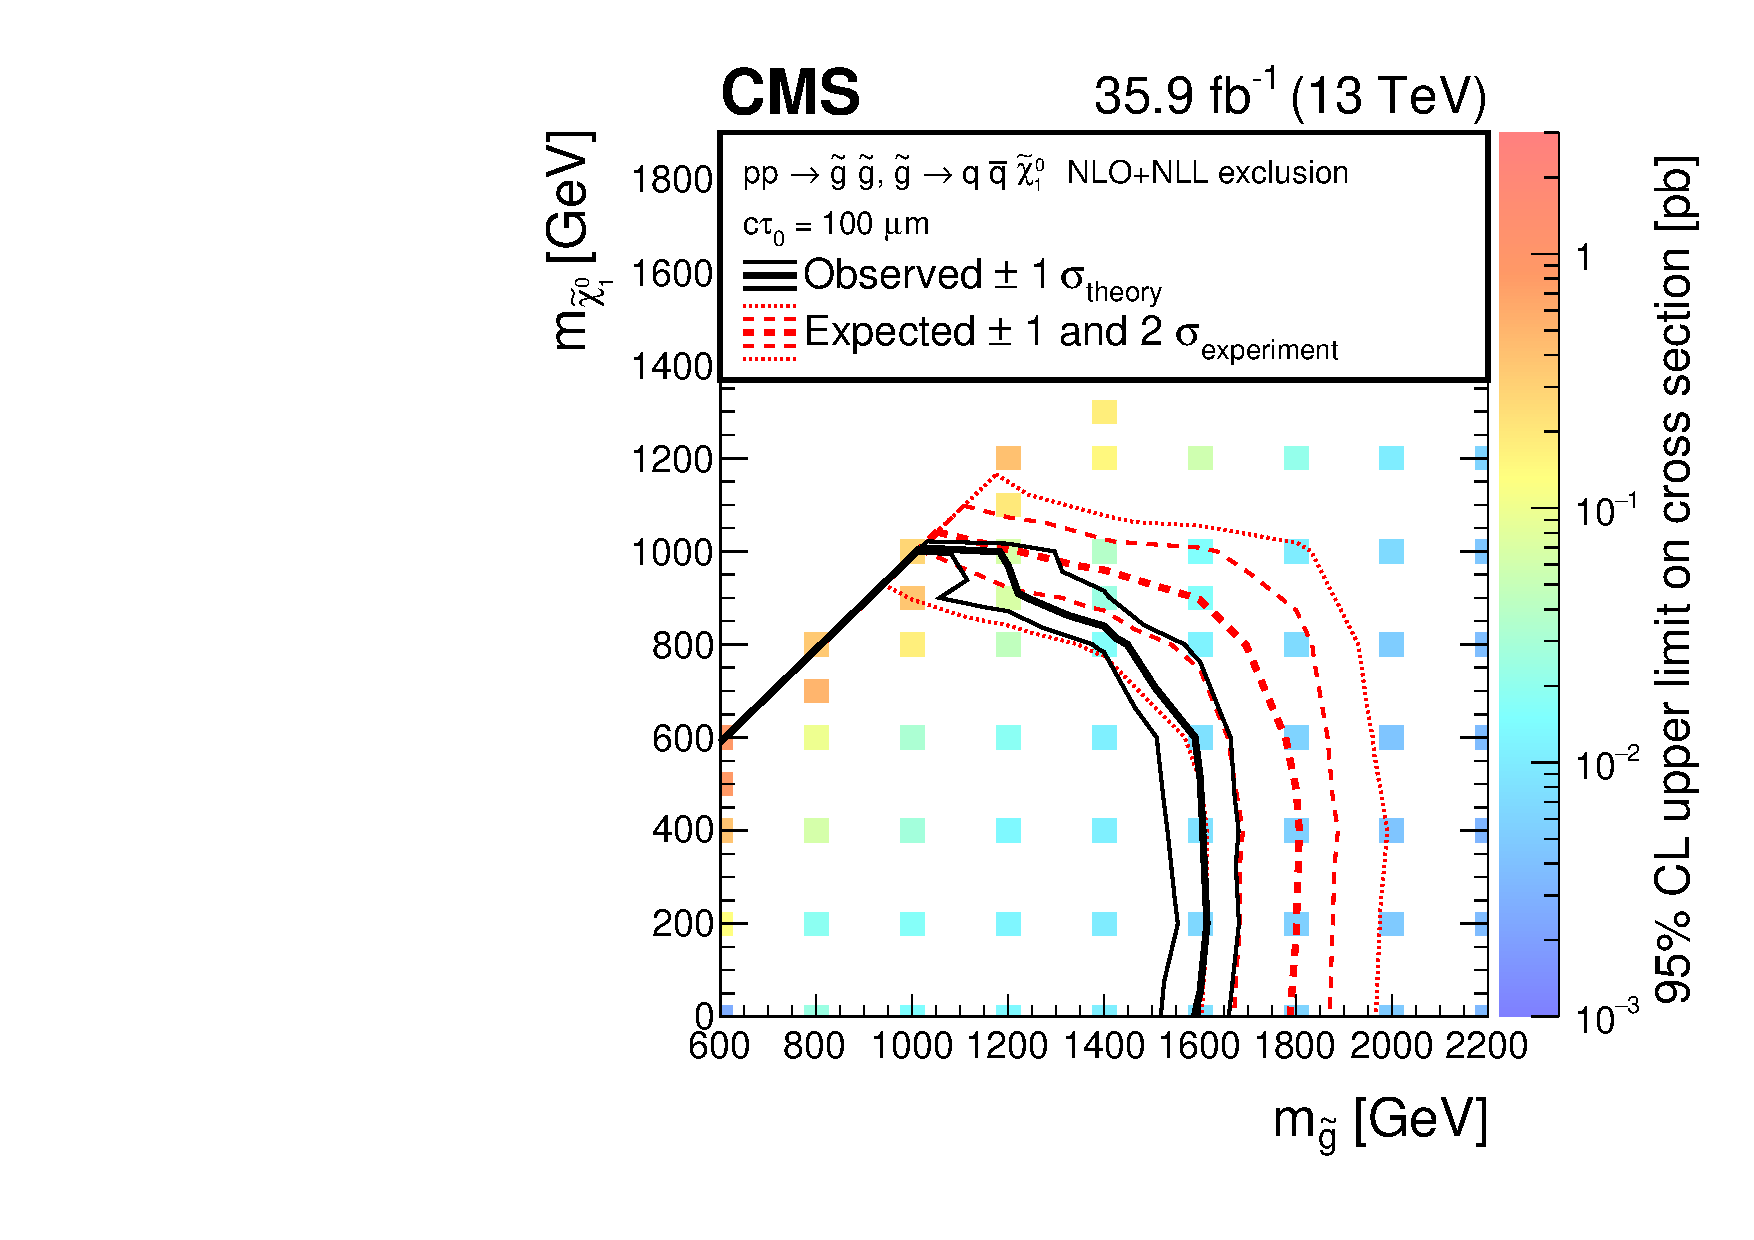
\includegraphics[width=0.49\textwidth]{figs/results/T1qqqqLL0p1XSEC}
\caption{Observed upper limit in cross section at 95\% confidence level 
(indicated by the colour scale) as a function of the \gluino~and 
\neutralino~masses for the Split SUSY simplified models. Each subfigure 
represents a different gluino lifetime. The thick (thin) black line indicates 
the observed excluded region assuming the nominal ($\pm1\sigma$ in theoretical 
cross section uncertainty) production cross section. The red dashed (dashed and 
dotted) represents the median ($\pm1\sigma$ and $\pm2\sigma$ in experimental 
uncertainty) expected excluded region.}
\label{fig:limits-individual-1}
\end{figure}
\begin{figure}[!t]
\centering
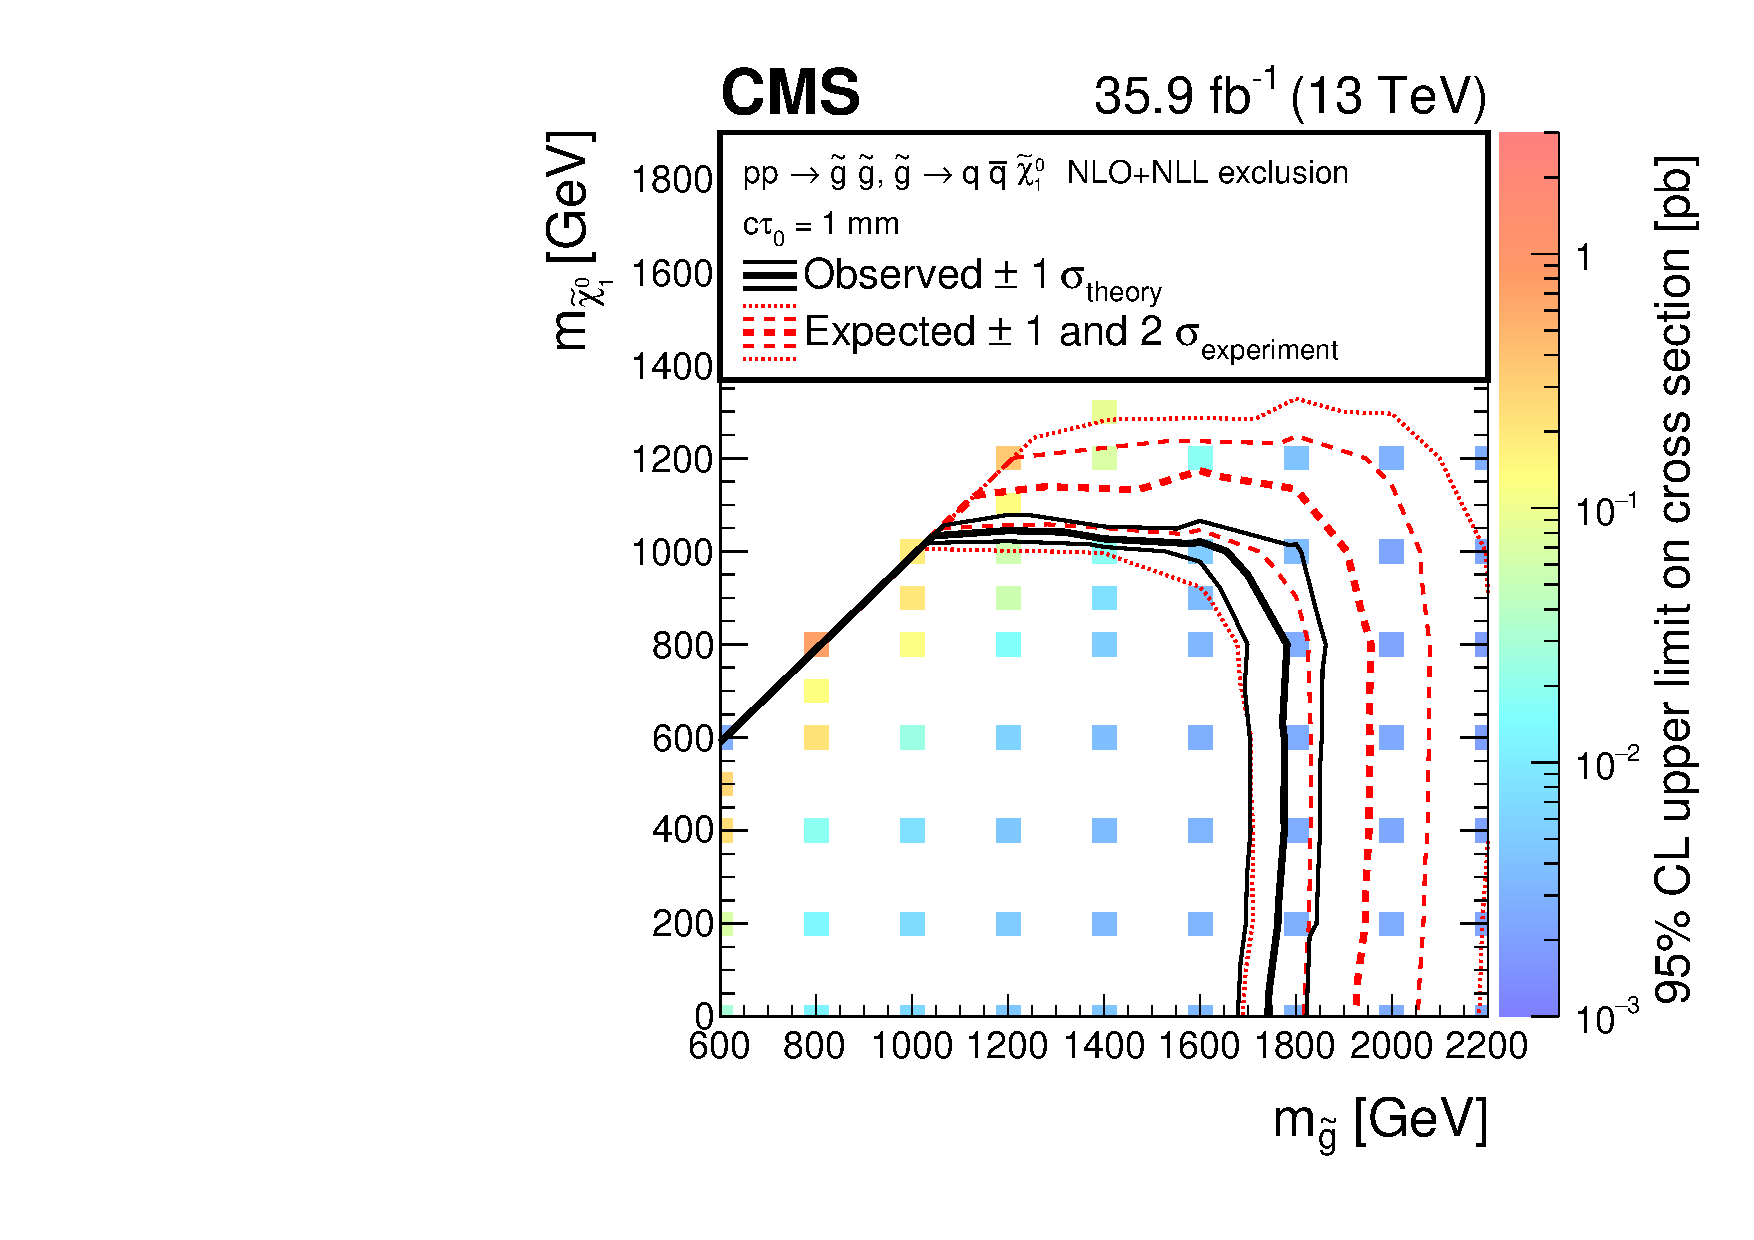
\includegraphics[width=0.49\textwidth]{figs/results/T1qqqqLL1XSEC}~
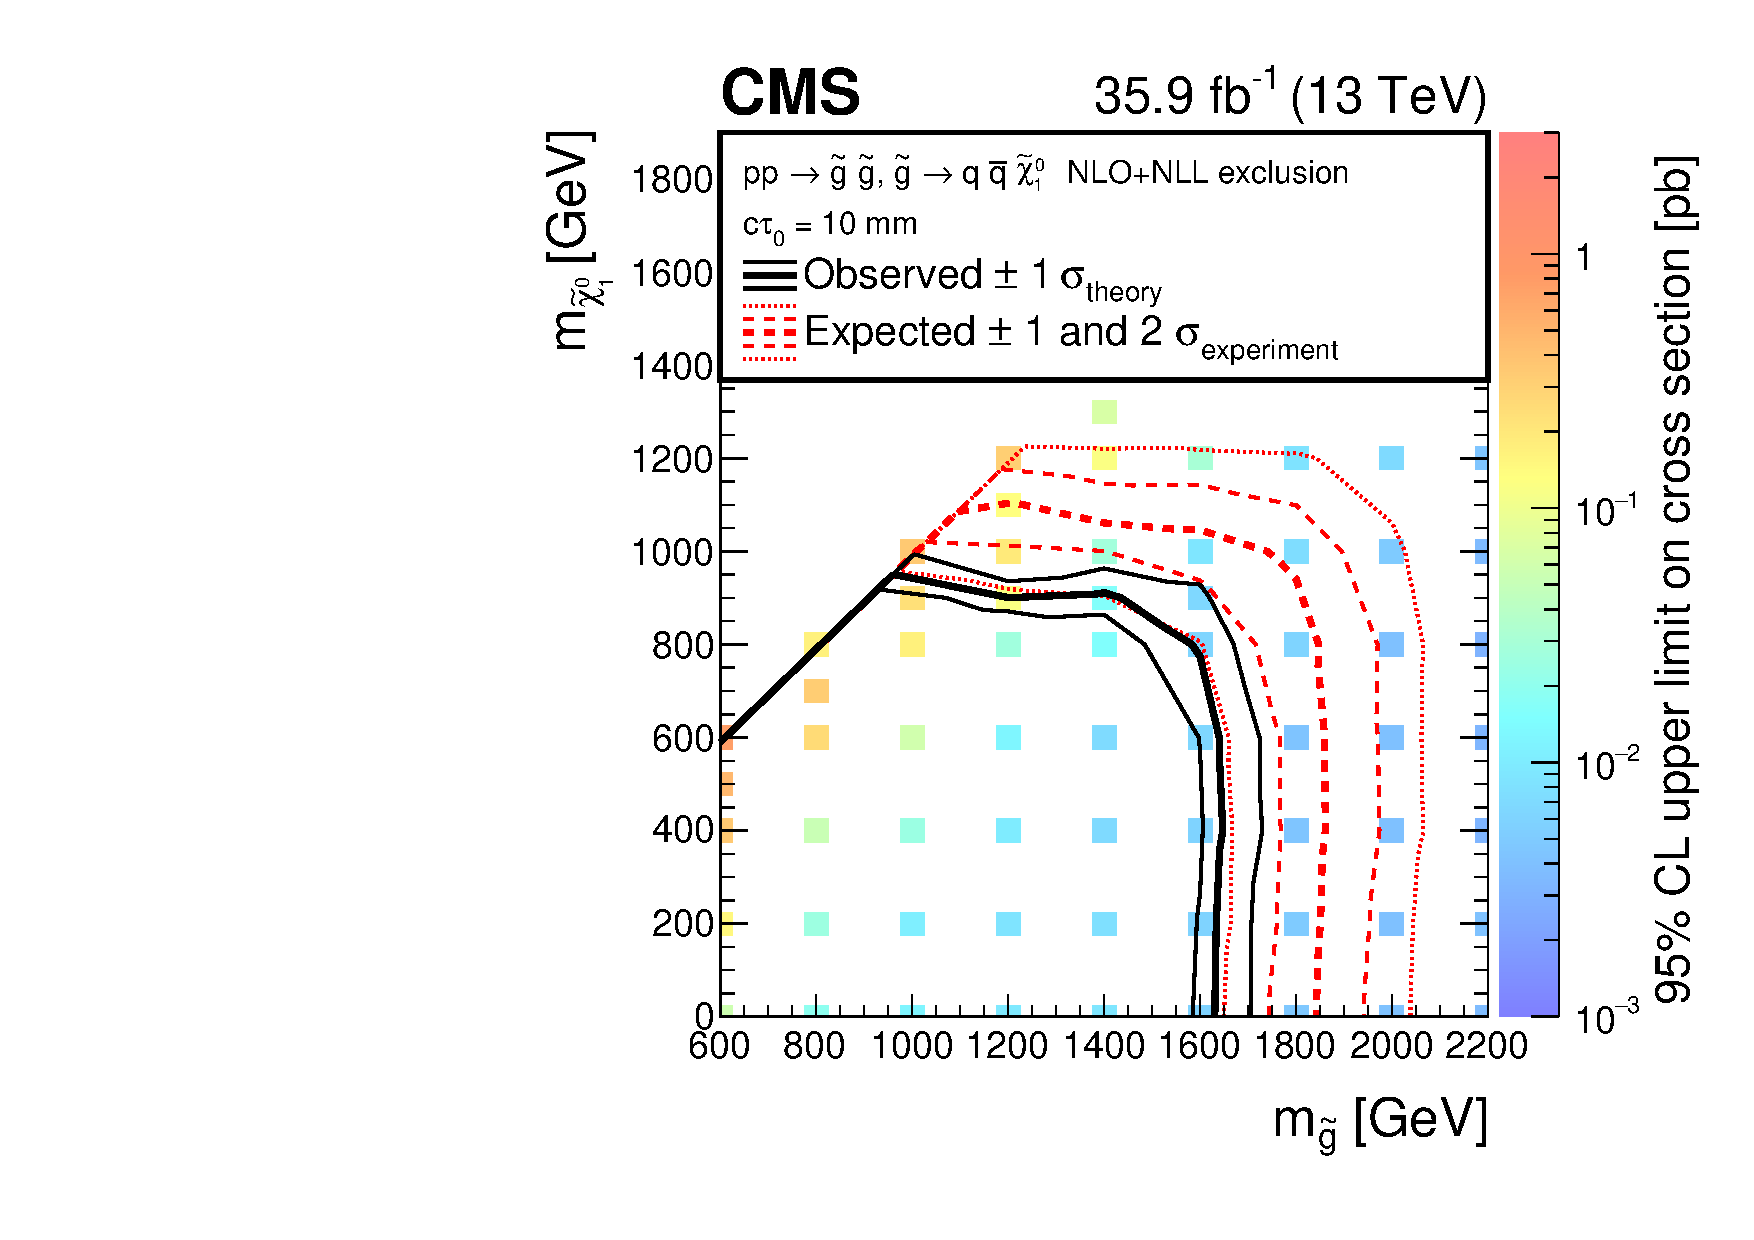
\includegraphics[width=0.49\textwidth]{figs/results/T1qqqqLL10XSEC}\\
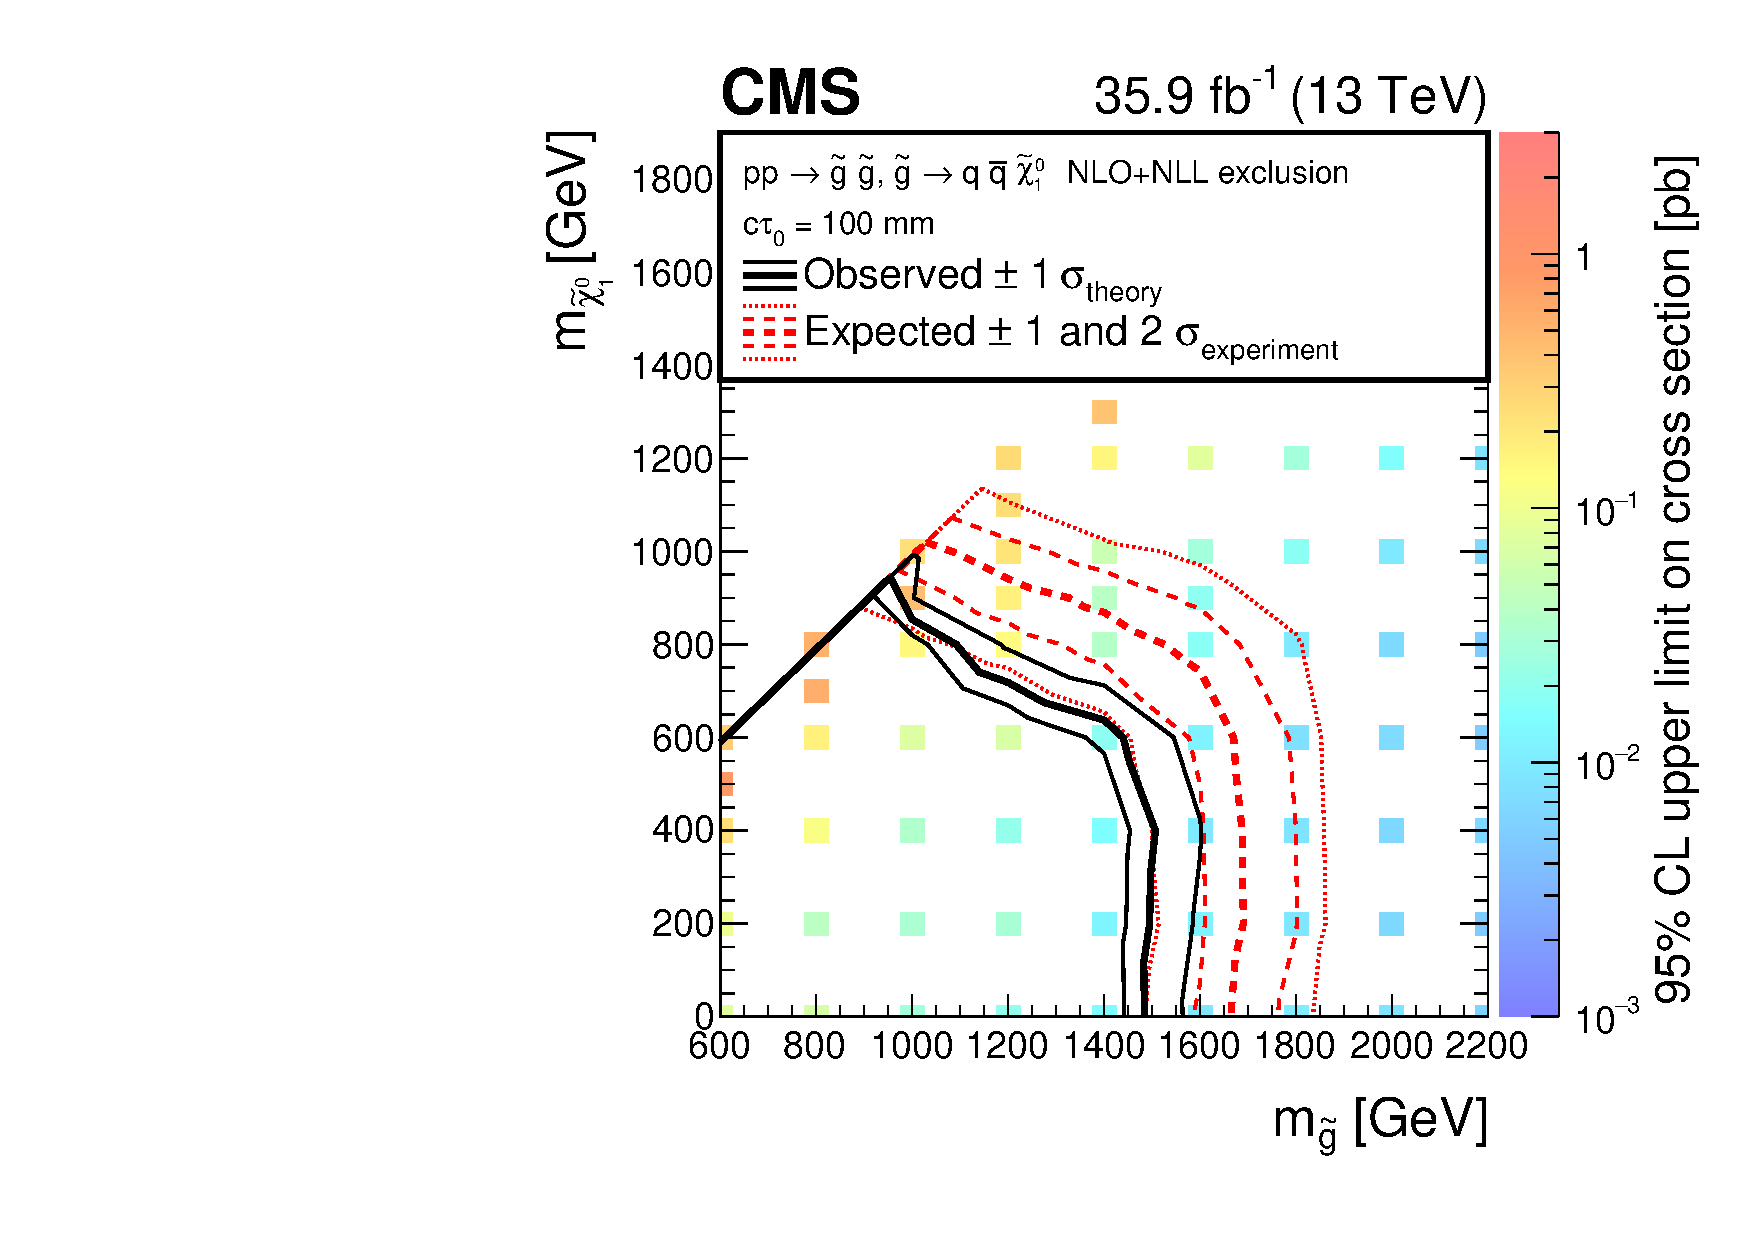
\includegraphics[width=0.49\textwidth]{figs/results/T1qqqqLL100XSEC}~
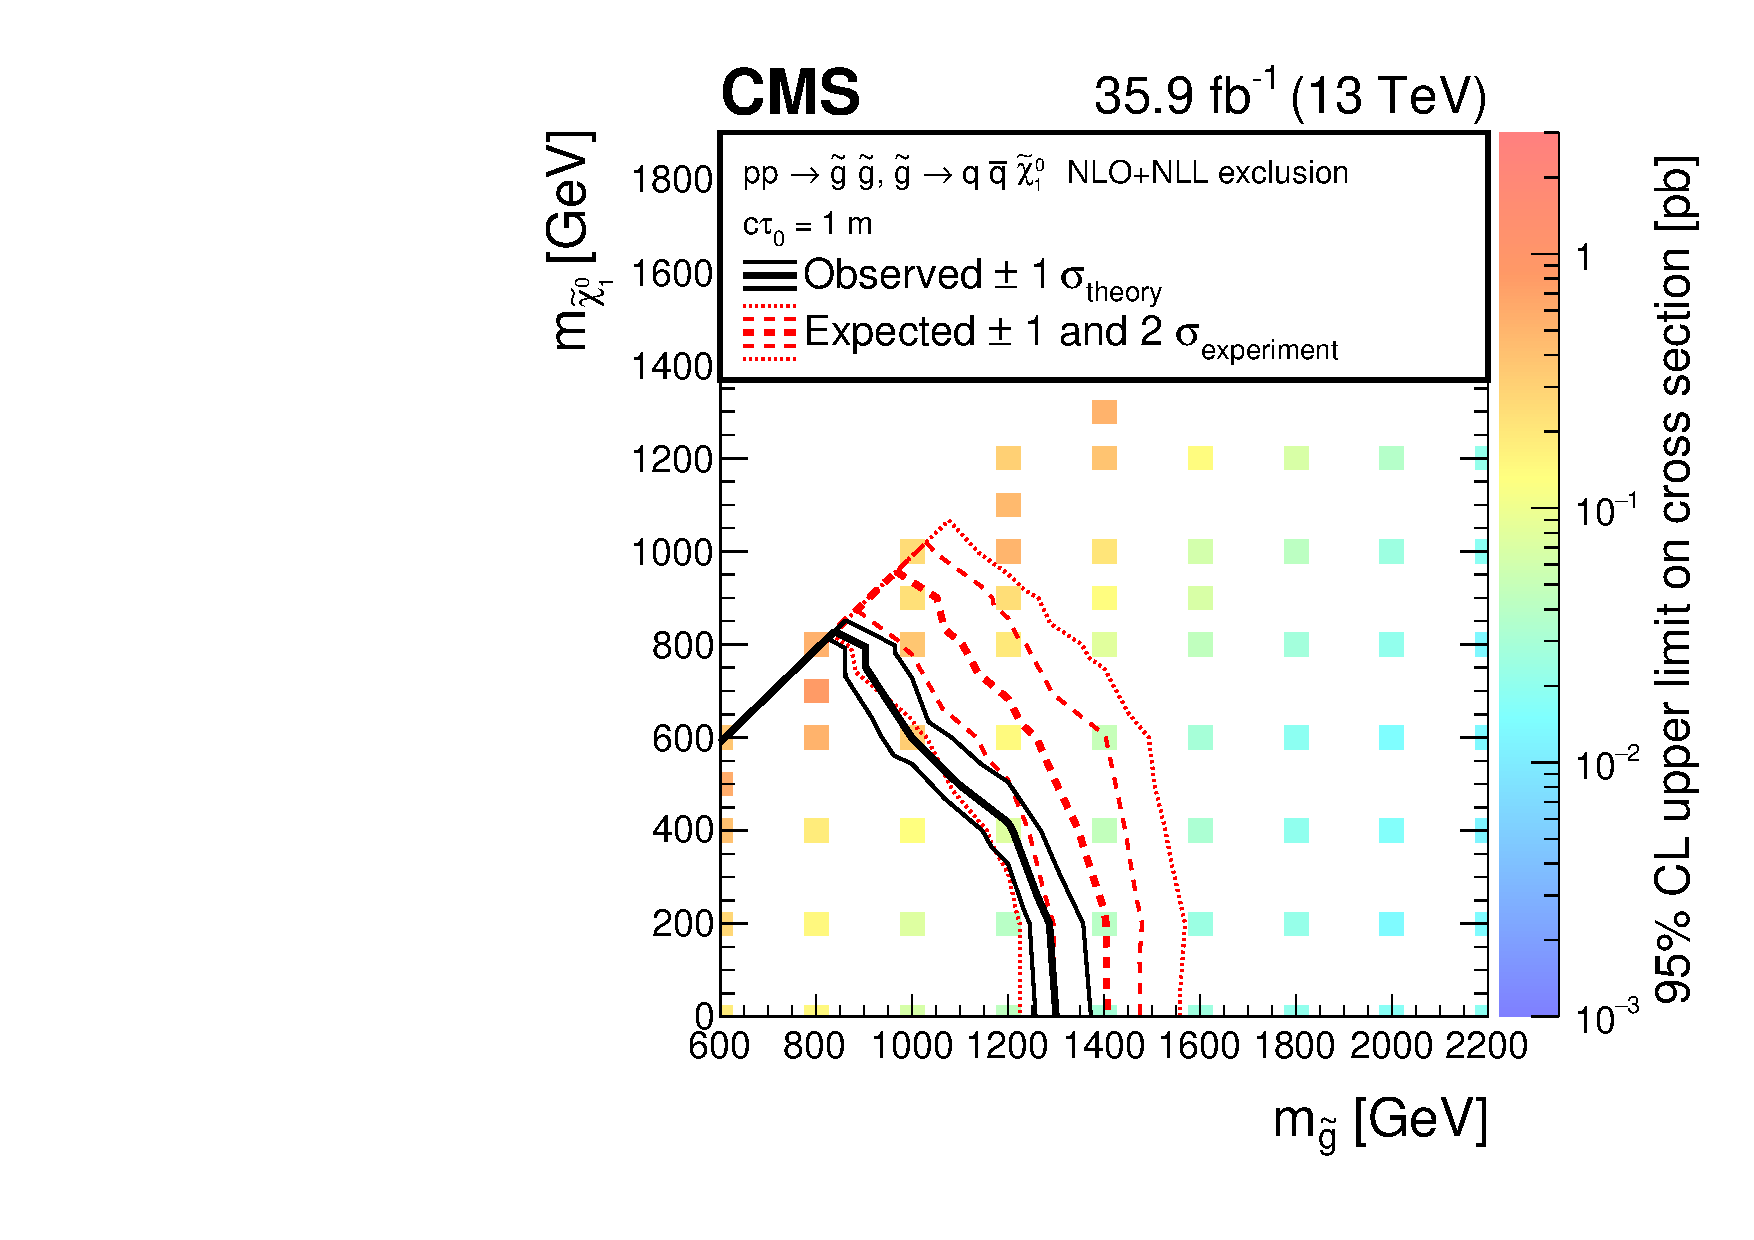
\includegraphics[width=0.49\textwidth]{figs/results/T1qqqqLL1000XSEC}
\caption{Observed upper limit in cross section at 95\% confidence level 
(indicated by the colour scale) as a function of the \gluino~and 
\neutralino~masses for the Split SUSY simplified models. Each subfigure 
represents a different gluino lifetime. The thick (thin) black line indicates 
the observed excluded region assuming the nominal ($\pm1\sigma$ in theoretical 
cross section uncertainty) production cross section. The red dashed (dashed and 
dotted) represents the median ($\pm1\sigma$ and $\pm2\sigma$ in experimental 
uncertainty) expected excluded region.}
\label{fig:limits-individual-2}
\end{figure}
\begin{figure}[!t]
\centering
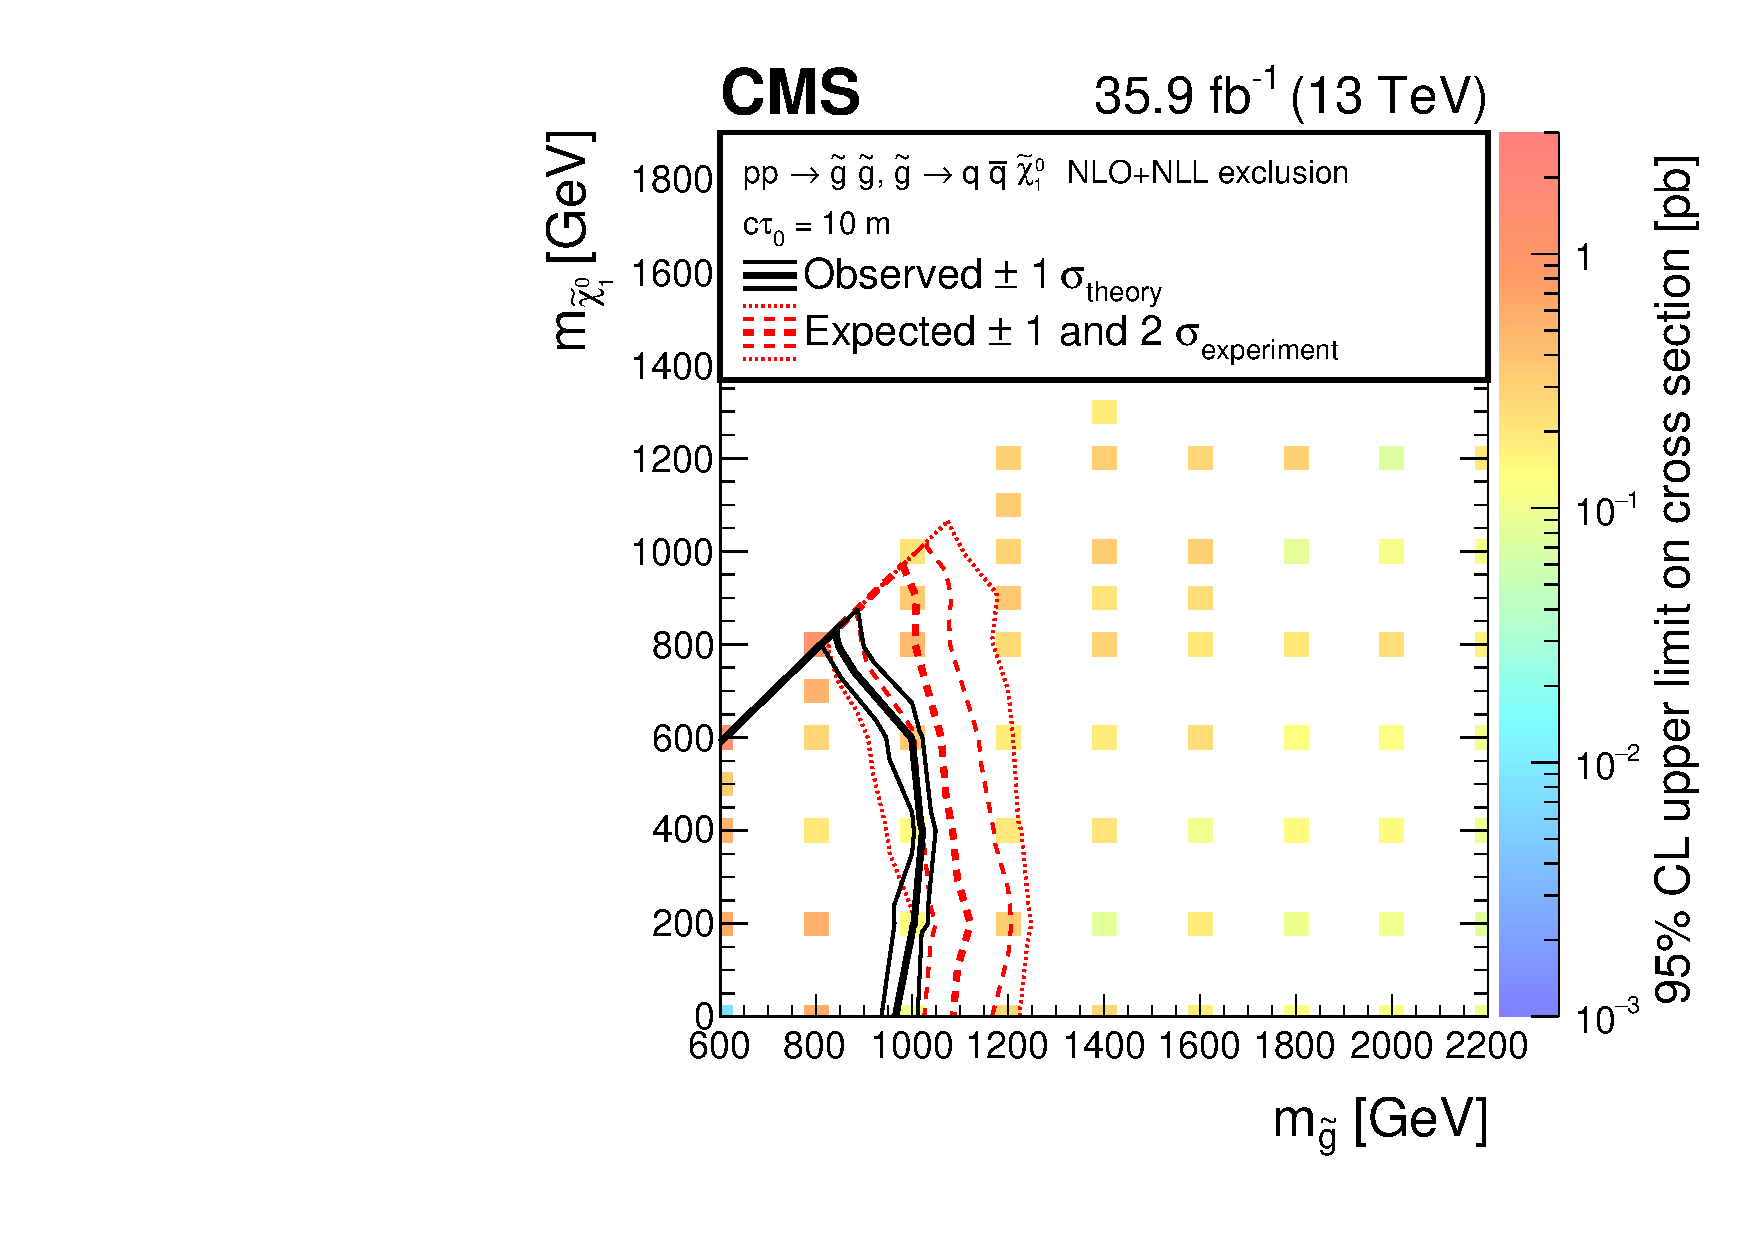
\includegraphics[width=0.49\textwidth]{figs/results/T1qqqqLL10000XSEC}~
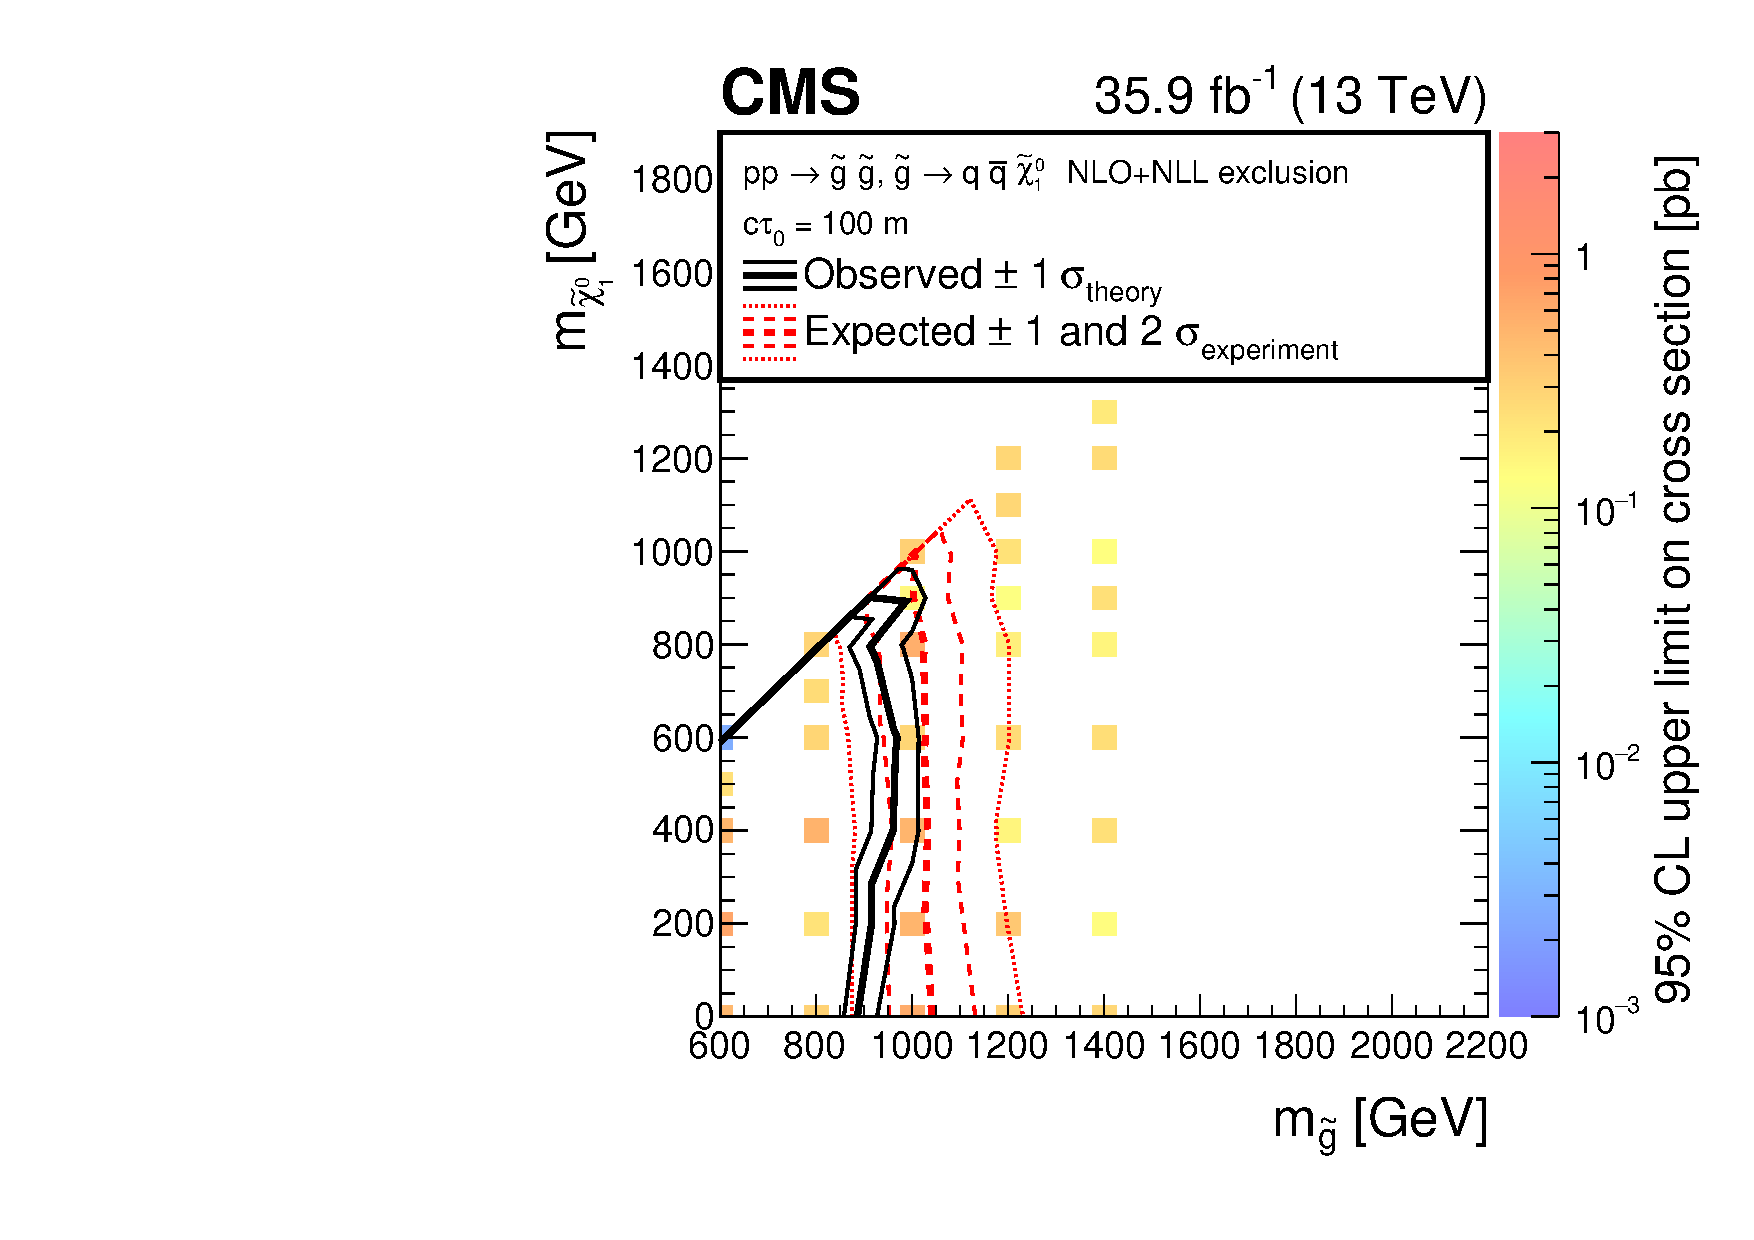
\includegraphics[width=0.49\textwidth]{figs/results/T1qqqqLL100000XSEC}\\
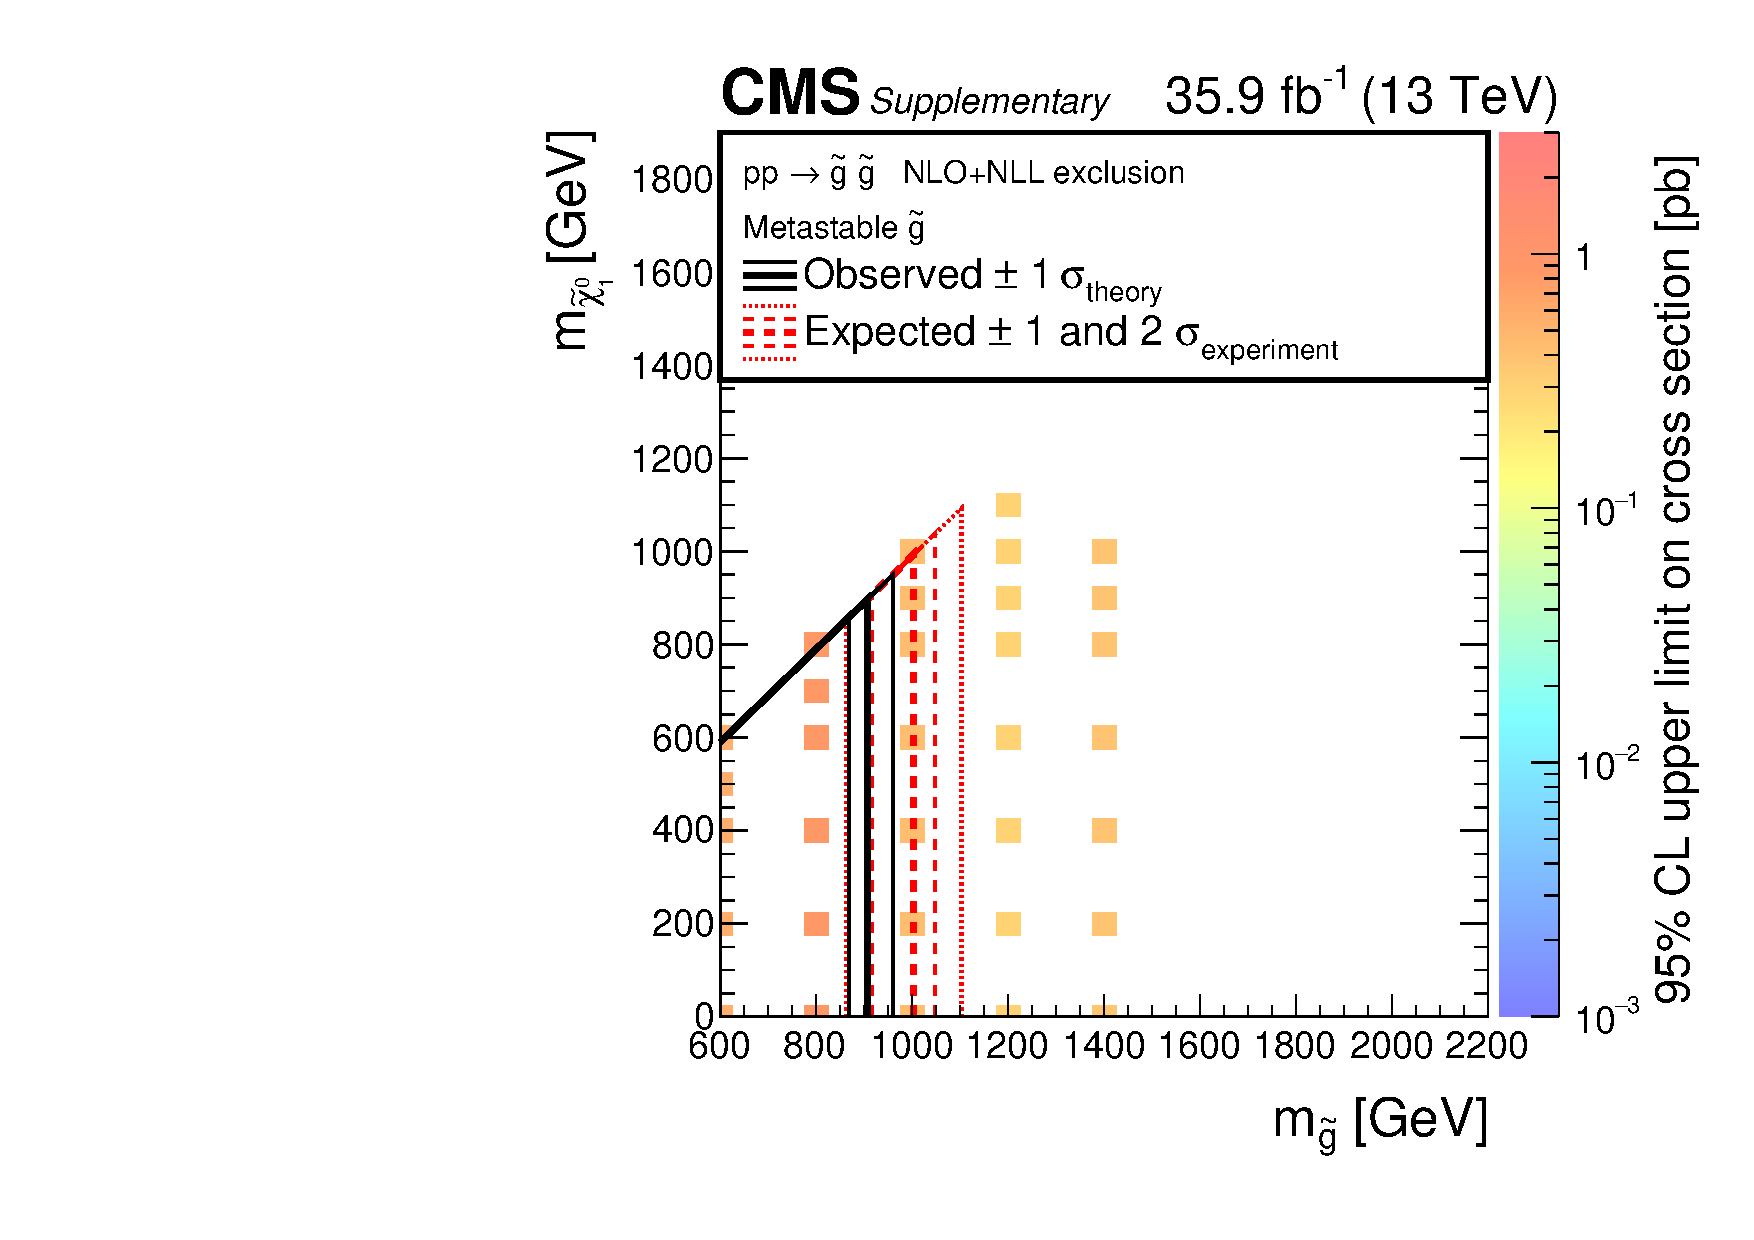
\includegraphics[width=0.49\textwidth]{figs/results/T1qqqqLLStableXSEC}
\caption{Observed upper limit in cross section at 95\% confidence level 
(indicated by the colour scale) as a function of the \gluino~and 
\neutralino~masses for the Split SUSY simplified models. Each subfigure 
represents a different gluino lifetime. The thick (thin) black line indicates 
the observed excluded region assuming the nominal ($\pm1\sigma$ in theoretical 
cross section uncertainty) production cross section. The red dashed (dashed and 
dotted) represents the median ($\pm1\sigma$ and $\pm2\sigma$ in experimental 
uncertainty) expected excluded region.}
\label{fig:limits-individual-3}
\end{figure}
\begin{figure}[!t]
\centering
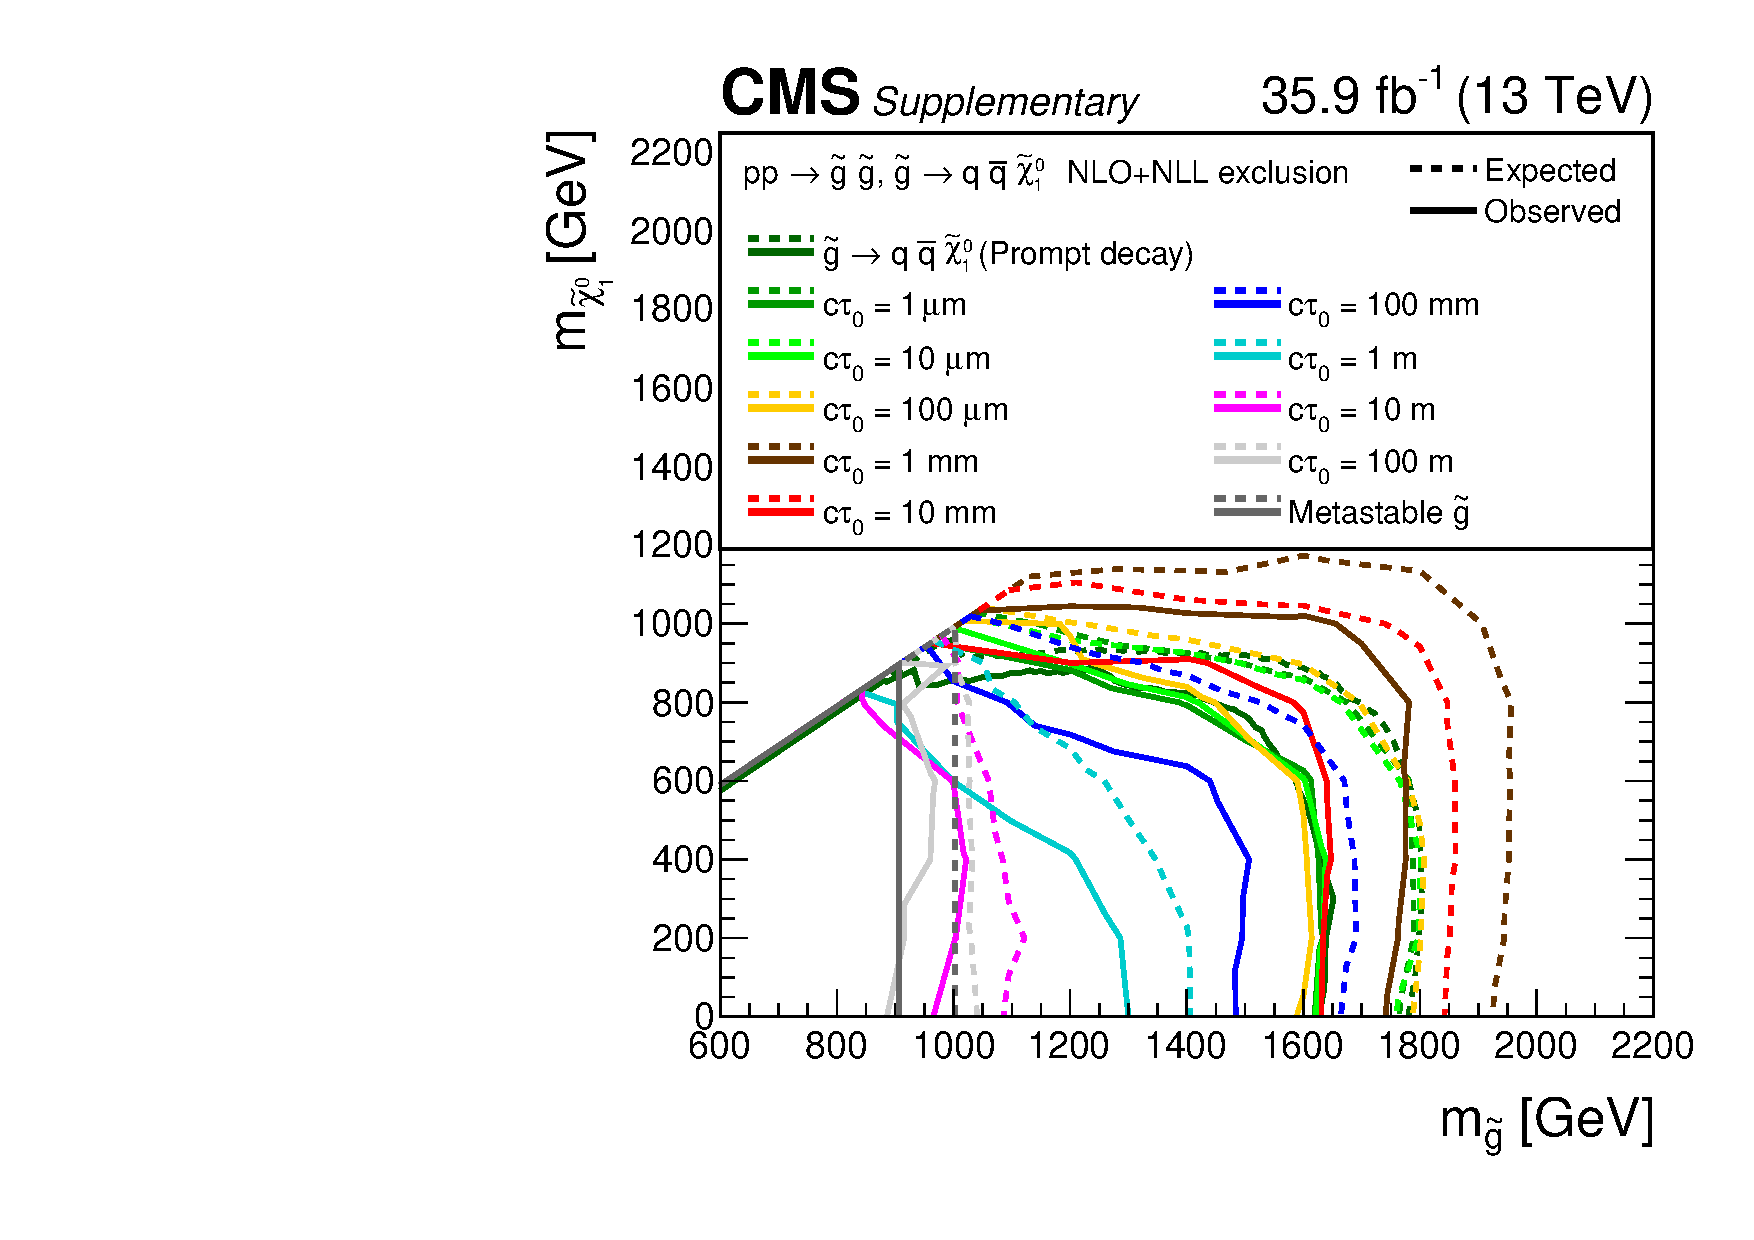
\includegraphics[width=0.8\textwidth]{figs/results/T1qqqqLLSummary}
\caption{Summary of observed and expected excluded regions at 95\% confidence 
level as a function of the \gluino~and \neutralino~masses for various gluino 
lifetimes for the Split SUSY simplified models.}
%\textbf{maybe just observed contours}}
\label{fig:limits-summary} 
\end{figure}

\begin{comment}
Chapter 5 – Results and interpretations (30%)
statistics section:
describe hypothesis testing, power, significance, neyman-pearson, Wilks’ theorem
maybe also parameter estimation, confidence intervals, goodness of fit
see Wardle and Gilbert theses
Simplified model distributions? i.e. describe the phenomenology
Estimated background vs observed data, studies of signal models (e.g. 
distributions, yields, efficiencies), description of statistical 
analysis/testing, limits on DM (vector, axial-vector, scalar, pseudoscalar, 
both light and heavy flavour production) and LL SUSY (T1qqqqLL) [and LL DM if 
arrives in time], comparison with dedicated searches
Mention/show most sensitive bins
Limits in ctau-mass plane?
Include/compare prompt gluino/stable chi2
Material interactions, reconstruction efficiency vs displacement, jet energy 
scale

%Acceptance times efficiency.
%Most sensitive bins.
%Some LL studies - in results section?

Limit planes ctau-mass?
Toy study?

DMLL: my presentations, raffaele, oliver exo workshop (future prospects).
Take home message: (see presentation - lack of coverage for models with 
compressed (N2,N1) and small ctau). Prompt search retains some sensitivity 
for long (short) gluino (DM) lifetimes (and is the most sensitive sub-cm and 
lifetimes beyond the detector, hence continue with prompt search in future), 
although clearly could be improved with a dedicated search/tagger as shown by 
the b-tag effects. Also compressed DM can be much improved by removing dphi cut.

DMLL useful presentation (eg slide 11)
%https://indico.cern.ch/event/671803/contributions/2782601/attachments/1568796/2473998/2017-11-31_exo_lldm.pdf
\end{comment}